\chapter{Validazione Sperimentale e Analisi dei Risultati}
\label{chap:validazione_sperimentale}

\section{Setup Sperimentale e Metodologia di Benchmark}
\label{sec:setup_sperimentale}

La valutazione empirica del framework multi-agente e l'indagine critica sulle metriche di valutazione automatica sono state condotte su un corpus eterogeneo e altamente rappresentativo di librerie open-source C e C++ di livello industriale ampiamente adottate nel software di sistema:
\begin{itemize}
    \item \textbf{TinyXML-2}: Parser XML moderno in C++ orientato alle massime prestazioni e all'efficienza di allocazione tramite pool interni di memoria, caratterizzato da strutture ad albero gerarchiche e grafi complessi di puntatori mutabili (\texttt{XMLDocument}, \texttt{XMLElement}, \texttt{XMLNode}).
    \item \textbf{sds (Simple Dynamic Strings)}: Libreria di stringhe dinamiche in C sviluppata per il core di Redis, basata su un layout binario di memoria non convenzionale con metadati di controllo (\emph{header} tipizzati) posizionati a offset negativi rispetto al puntatore stringa visibile.
    \item \textbf{cJSON}: Parser e generatore JSON ultra-leggero in puro C ANSI, fondato su strutture ricorsive ad albero con allocazione dinamica esplicita e puntatori \emph{parent-child/next-prev}.
    \item \textbf{miniz}: Implementazione di compressione lossless compatibile con zlib e Deflate contenuta in un singolo file sorgente, fortemente dipendente da buffer lineari, aritmetica dei puntatori a byte grezzi e bit-manipulation.
    \item \textbf{http-parser}: Motore di parsing HTTP asincrono e guidato da macchina a stati finiti (FSM), originariamente implementato per Node.js.
    \item \textbf{OpenCV (core)} e \textbf{fmt}: Moduli matematici e di formattazione stringhe ad alta efficienza per l'estrazione e verifica di contratti tipizzati complessi.
\end{itemize}

\subsection{Strategie di Campionamento e Controllo Sperimentale}
Per garantire l'imparzialità statistica dell'estrazione dei campioni ed eludere bias di selezione favorevoli a funzioni banali (quali getter/setter monoriga o wrapper privi di ramificazioni), il framework prevede tre distinte modalità operative:
\begin{enumerate}
    \item \textbf{Campionamento Stratificato per Complessità (LOC / AST Depth)}: partiziona l'insieme delle funzioni estratte in fasce dimensionali (\emph{short}: $< 15$ LOC, \emph{medium}: $15-50$ LOC, \emph{complex}: $> 50$ LOC), estraendo un numero bilanciato di campioni per ciascun strato.
    \item \textbf{Campionamento Casuale Pseudo-Deterministico}: adotta un seed globale fisso ($\text{seed} = 40$) al fine di garantire la totale riproducibilità dei run sperimentali cross-modello e consentire confronti differenziali rigorosi.
    \item \textbf{Campionamento Sequenziale Topologico}: estrae le funzioni rispettando l'ordine topologico del grafo delle dipendenze di compilazione della code-base.
\end{enumerate}

Il benchmark di validazione di sistema analizzato nel presente capitolo è stato eseguito con campionamento pseudo-deterministico su un set diversificato di 15 funzioni ad elevata complessità contrattuale (riproducibile mediante \texttt{python utils/benchmark\_eval.py -l all -n 15 -m multiagent --sampling random --seed 40 --roundtrip}).

In parallelo, per condurre un'analisi comparativa delle metriche senza fattori confondenti, è stata istanziata una suite di test controllati multilivello, coprente 5 classi semantiche essenziali (\emph{EQUIVALENT}, \emph{ADVERSARIAL}, \emph{DOMAIN\_SIMILAR}, \emph{ORTHOGONAL}, \emph{FLUFF\_VERBOSITY}) applicate ad armi pari sia al dominio naturale (\emph{Doc vs Doc}) sia a quello del codice sorgente (\emph{C vs C}, \emph{Python vs Python}, \emph{C vs Python}), oltre a specifici stress test avversari e test di troncamento di contesto.

---

\section{Analisi Comparativa delle Rappresentazioni (Cross-Modal)}
\label{sec:analisi_cross_modal}

\begin{figure}[htbp]
    \centering
    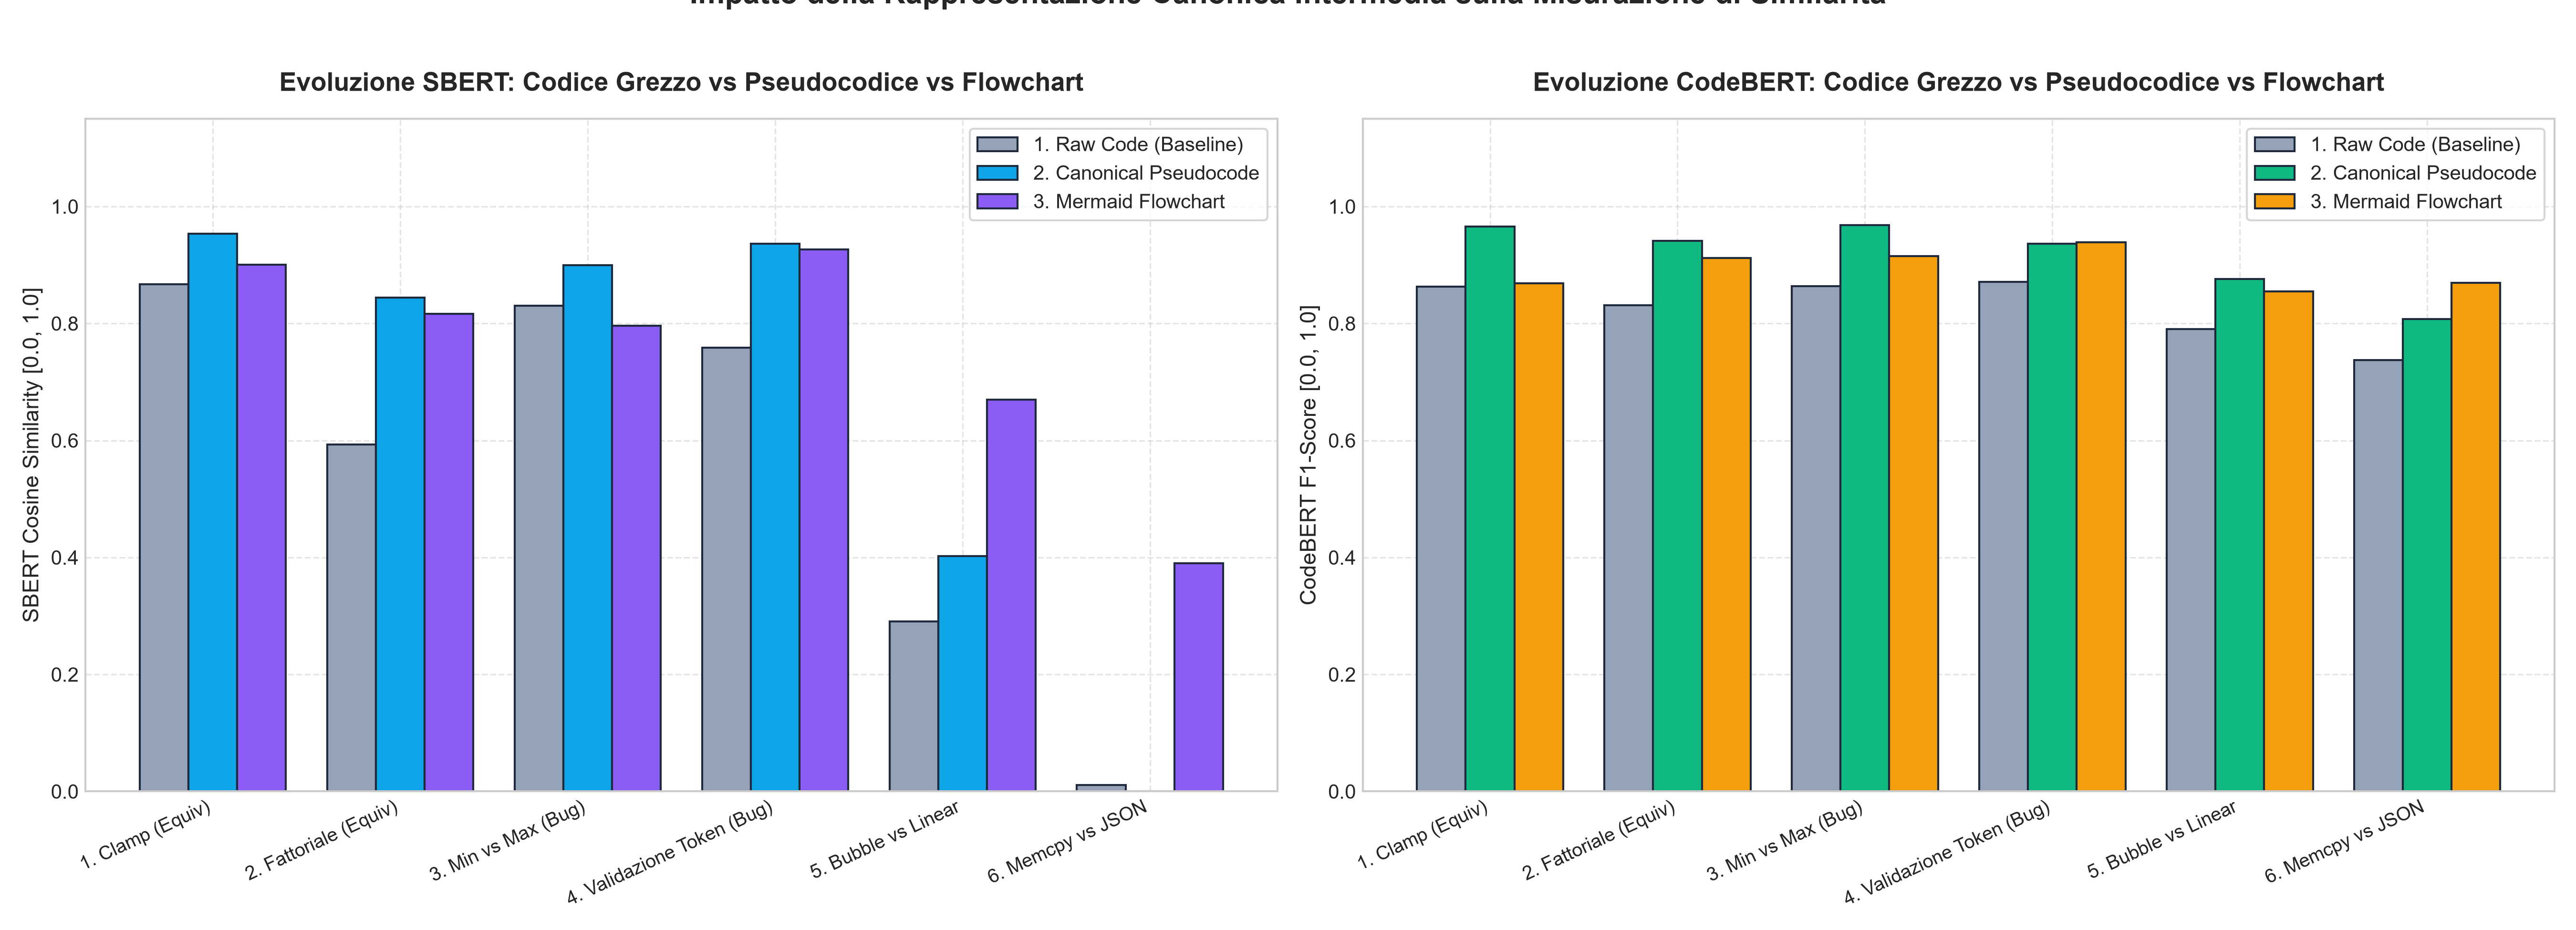
\includegraphics[width=0.85\linewidth]{figures/canonical_vs_raw_comparison.png}
    \caption{Confronto di allineamento semantico (SBERT, BERTScore, CodeBERTScore e ROUGE-L) tra le rappresentazioni: Raw Code, Canonical Pseudocode e Mermaid Flowchart.}
    \label{fig:canonical_vs_raw}
\end{figure}

Un interrogativo scientifico centrale riguarda la capacità dei modelli di embedding di confrontare entità eterogenee, colmando il divario tra la sintassi imperativa del linguaggio sorgente (C/C++) e il testo esplicativo o la trasposizione in linguaggi di alto livello (Python). A tale scopo, sulla scia degli studi sulle rappresentazioni strutturate del codice \cite{alon_code2seq_2019,guo_graphcodebert_2021}, sono state investigate quattro distinte modalità di rappresentazione:
\begin{enumerate}
    \item \textbf{Raw Code (Baseline)}: codice C nativo confrontato direttamente con codice Python o Doxygen senza alcuna pre-elaborazione.
    \item \textbf{Canonical Pseudocode}: normalizzazione algoritmica intermedia generata eliminando il rumore sintattico (parentesi graffe, convenzioni di tipizzazione statica, macro) ed evidenziando i flussi di controllo fondamentali (\texttt{IF-THEN-ELSE}, \texttt{WHILE}, \texttt{RETURN}), riprendendo i principi di rappresentazione schematica del flusso logico dei programmi \cite{robillard_schematic_1986}.
    \item \textbf{Mermaid Flowchart}: rappresentazione puramente topologica del grafo di flusso di controllo (CFG), codificata sotto forma di nodi decisionali e archi orientati.
    \item \textbf{Docstring / Doxygen}: specifica dichiarativa in linguaggio naturale strutturato.
\end{enumerate}

I dati sperimentali raccolti su casi di studio controllati sono riassunti nella \Cref{tab:cross_modal_results}.

\begin{table}[htbp]
\centering
\footnotesize
\setlength{\tabcolsep}{3pt}
\caption{Confronto quantitativo multi-rappresentazione attraverso diverse classi di equivalenza logica.}
\label{tab:cross_modal_results}
\begin{tabular}{p{3.2cm}lcccc}
\toprule
\textbf{Caso di Studio} & \textbf{Rappresentazione} & \textbf{SBERT} & \textbf{BERT F1} & \textbf{CodeBERT} & \textbf{ROUGE-L} \\
\midrule
\multirow{3}{=}{\textbf{Clamp Valore}\\(\emph{Equiv.}: C \texttt{if} vs Py \texttt{min/max})}
  & Raw Code (Baseline) & 0.867 & 0.791 & 0.863 & 0.571 \\
  & Canonical Pseudocode & \textbf{0.953} & \textbf{0.951} & \textbf{0.966} & \textbf{0.850} \\
  & Mermaid Flowchart & 0.901 & 0.781 & 0.869 & 0.412 \\
\midrule
\multirow{3}{=}{\textbf{Fattoriale}\\(\emph{Equiv.}: C \texttt{for} vs Py \texttt{math.prod})}
  & Raw Code (Baseline) & 0.593 & 0.645 & 0.831 & 0.400 \\
  & Canonical Pseudocode & \textbf{0.844} & \textbf{0.857} & \textbf{0.942} & \textbf{0.522} \\
  & Mermaid Flowchart & 0.816 & 0.828 & 0.912 & 0.518 \\
\midrule
\multirow{3}{=}{\textbf{Min vs Max (Bug)}\\(\emph{Advers.}: \texttt{<} vs \texttt{>})}
  & Raw Code (Baseline) & 0.830 & 0.740 & 0.864 & 0.609 \\
  & Canonical Pseudocode & 0.900 & 0.897 & 0.968 & 0.929 \\
  & Mermaid Flowchart & 0.796 & 0.845 & 0.915 & 0.567 \\
\midrule
\multirow{3}{=}{\textbf{Bubble Sort C vs Py Search}\\(\emph{Domain Similar})}
  & Raw Code (Baseline) & 0.291 & 0.626 & 0.791 & 0.286 \\
  & Canonical Pseudocode & 0.402 & 0.737 & 0.876 & 0.421 \\
  & Mermaid Flowchart & 0.670 & 0.722 & 0.855 & 0.165 \\
\midrule
\multirow{3}{=}{\textbf{Memcpy C vs JSON Py}\\(\emph{Orthogonal})}
  & Raw Code (Baseline) & 0.011 & 0.551 & 0.738 & 0.000 \\
  & Canonical Pseudocode & 0.000 & 0.547 & 0.807 & 0.000 \\
  & Mermaid Flowchart & 0.390 & 0.744 & 0.869 & 0.138 \\
\bottomrule
\end{tabular}
\end{table}

\subsection{Analisi di CodeBERT vs SBERT/BERTScore: Resilienza Sintattica vs Cecità Semantica}
L'esame incrociato dei risultati in \Cref{tab:cross_modal_results} e in \Cref{fig:canonical_vs_raw} evidenzia comportamenti strutturalmente divergenti tra le metriche concepite per il testo e i modelli pre-addestrati bilingui:
\begin{itemize}
    \item \textbf{Degradazione di SBERT sul codice grezzo}: Nei confronti cross-linguaggio (C vs Python) su funzioni equivalenti, come il calcolo del Fattoriale iterativo in C rispetto all'invocazione di \texttt{math.prod} in Python, SBERT crolla a un modesto punteggio di $0.593$ a causa della disparità lessicale superficiale. Quando il codice viene preventivamente proiettato nella forma di \emph{Canonical Pseudocode}, SBERT sale significativamente a $0.844$ ($+0.251$), e ROUGE-L passa da $0.400$ a $0.522$.
    \item \textbf{Elevata sensibilità inter-linguistica di CodeBERTScore}: A differenza di SBERT, CodeBERT (pre-addestrato congiuntamente con compiti di Masked Language Modeling su corpora bilingui Natural Language/Programming Language) mantiene punteggi di $F_1$ eccezionalmente stabili già sul codice sorgente grezzo ($0.831$ sul Fattoriale grezzo, che sale a $0.942$ in pseudocodice). Ciò dimostra che CodeBERT proietta le primitive del linguaggio imperativo in una geometria concettuale comune indipendente dal target sintattico.
    \item \textbf{Il Fallimento Sistemico sui Casi Adversarial}: La normalizzazione in pseudocodice, sebbene benefica nel risolvere la varianza sintattica, \textbf{esacerba drammaticamente la vulnerabilità neurale sui bug di inversione logica}. Nel caso adversarial (ricerca del minimo con operatore corretto \texttt{<} rispetto a ricerca del massimo con bug invertito \texttt{>}), lo pseudocodice aumenta la similarità di CodeBERT da $0.864$ a un vertiginoso $0.968$, e quella di SBERT da $0.830$ a $0.900$. Poiché lo pseudocodice elimina ogni divergenza di contorno focalizzando il testo sul puro corpo comune a eccezione di un singolo operatore relazionale, le rappresentazioni dense collocano le due funzioni a distanza quasi nulla nello spazio euclideo.
\end{itemize}

---

\section{Valutazione Sperimentale ad Armi Pari delle Metriche NLP}
\label{sec:valutazione_armi_pari_nlp}

Un principio metodologico cardine della presente tesi consiste nel \textbf{valutare tutte le metriche ad armi pari}. Nella letteratura sul code summarization, metriche concepite specificamente per il testo naturale (quali Sentence-BERT, BERTScore, METEOR o BLEURT) vengono sovente applicate acriticamente alla documentazione, ignorando cosa accade quando le medesime metriche vengono poste a confronto diretto con il codice sorgente (coppie \emph{C vs C}), oppure quando metriche nate per il codice (CodeBERTScore) operano su coppie testuali (\emph{Doc vs Doc}).

A tale scopo è stato allestito un benchmark controllato che interroga ciascuna metrica attraverso cinque classi semantiche ben distinte, ripetute sistematicamente su molteplici domini rappresentativi:
\begin{enumerate}
    \item \textbf{EQUIVALENT}: Logica identica espressa con costrutti differenti (es. Fibonacci iterativo vs ricorsivo in C; parafrasi formale Doxygen vs descrizione naturale discorsiva in Doc).
    \item \textbf{ADVERSARIAL}: Identica quasi al 100\% sul piano lessicale, ma contenente un'inversione semantica distruttiva (es. calcolo Minimo \texttt{<} vs Massimo \texttt{>} in C; obbligo di rilascio memoria \texttt{must free} vs divieto fatale \texttt{must NOT free} in Doc).
    \item \textbf{DOMAIN\_SIMILAR}: Stesso dominio applicativo e medesimi tipi di dato, ma algoritmo differente (es. Binary Search vs Somma di elementi in un array in C; Quicksort vs Binary Search in Doc).
    \item \textbf{ORTHOGONAL}: Domini applicativi totalmente scorrelati e privi di intersezione funzionale (es. parsing di stringhe vs moltiplicazione di matrici in C; socket di rete TLS vs calcolo del determinante in Doc).
    \item \textbf{FLUFF\_VERBOSITY}: Logica essenziale identica ma immersa in un eccesso di codice ridondante (variabili temporanee, chiamate di logging) o in verbose allucinazioni descrittive non pertinenti generate da LLM.
\end{enumerate}

I dati sperimentali globali sono riassunti graficamente nella panoramica comparativa di \Cref{fig:nlp_metric_overview} e dettagliati analiticamente nella \Cref{tab:nlp_5classes_breakdown}.

\begin{figure}[htbp]
    \centering
    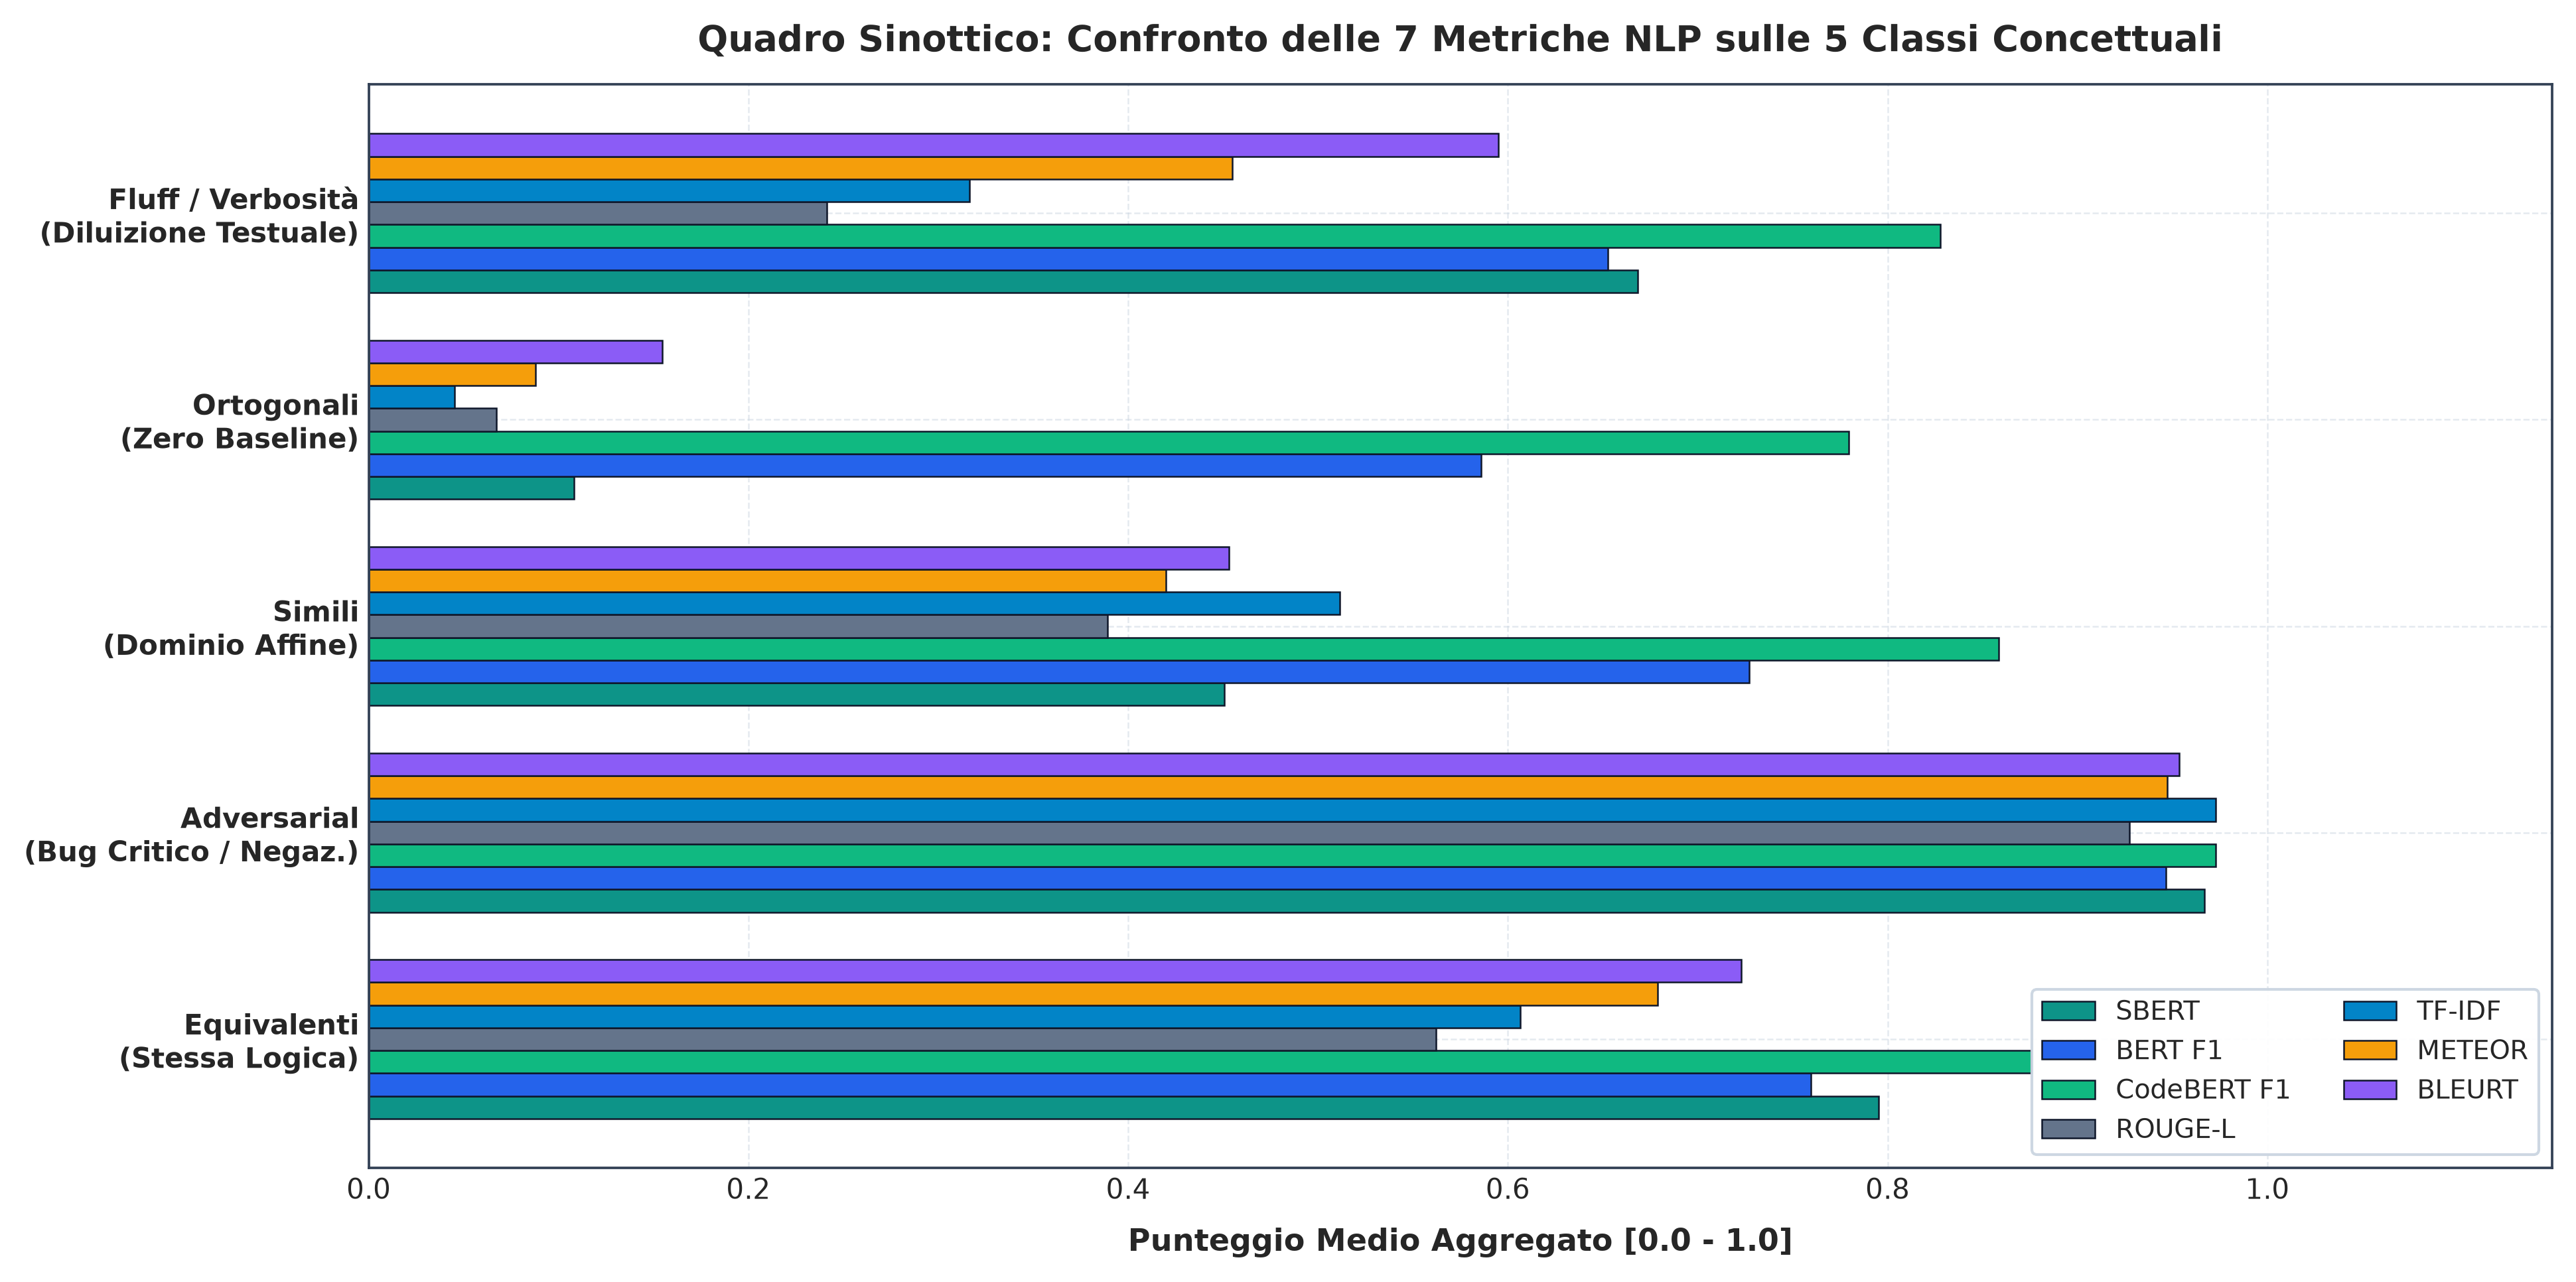
\includegraphics[width=0.95\linewidth]{figures/nlp_metric_overview_all_classes.png}
    \caption{Panoramica globale delle metriche NLP (SBERT, BERTScore, CodeBERT, ROUGE-L, TF-IDF, METEOR, BLEURT) attraverso le 5 classi semantiche, aggregando tutti i domini di test.}
    \label{fig:nlp_metric_overview}
\end{figure}

\begin{table}[htbp]
\centering
\scriptsize
\setlength{\tabcolsep}{2.5pt}
\caption{Confronto ad armi pari delle metriche NLP sui domini \emph{C vs C}, \emph{Doc vs Doc} e sulla media globale dei test.}
\label{tab:nlp_5classes_breakdown}
\begin{tabular}{llccccccc}
\toprule
\textbf{Classe Semantica} & \textbf{Dominio} & \textbf{SBERT} & \textbf{BERT\_F1} & \textbf{CodeBERT} & \textbf{ROUGE-L} & \textbf{TF-IDF} & \textbf{METEOR} & \textbf{BLEURT} \\
\midrule
\multirow{3}{*}{\textbf{EQUIVALENT}} 
  & C vs C (Fibonacci Iter vs Ric) & 0.862 & 0.829 & 0.896 & 0.800 & 0.859 & 0.831 & 0.798 \\
  & Doc vs Doc (Parafrasi Formale) & 0.637 & 0.556 & 0.776 & 0.246 & 0.280 & 0.441 & 0.507 \\
  & \emph{Media Globale (6 Domini)} & \emph{0.795} & \emph{0.760} & \emph{0.876} & \emph{0.562} & \emph{0.606} & \emph{0.679} & \emph{0.723} \\
\midrule
\multirow{3}{*}{\textbf{ADVERSARIAL}} 
  & C vs C (Min \texttt{<} vs Max \texttt{>}) & \textbf{0.984} & \textbf{0.991} & \textbf{0.997} & \textbf{1.000} & \textbf{1.000} & \textbf{0.992} & \textbf{0.990} \\
  & Doc vs Doc (\texttt{must} vs \texttt{must NOT free}) & \textbf{0.995} & \textbf{0.977} & \textbf{0.983} & \textbf{0.957} & \textbf{0.957} & \textbf{0.976} & \textbf{0.986} \\
  & \emph{Media Globale (6 Domini)} & \textbf{\emph{0.967}} & \textbf{\emph{0.947}} & \textbf{\emph{0.973}} & \textbf{\emph{0.928}} & \textbf{\emph{0.973}} & \textbf{\emph{0.947}} & \textbf{\emph{0.954}} \\
\midrule
\multirow{3}{*}{\textbf{DOMAIN\_SIMILAR}} 
  & C vs C (Search vs Sum Array) & 0.401 & 0.770 & 0.850 & 0.280 & 0.393 & 0.340 & 0.365 \\
  & Doc vs Doc (Quicksort vs Search) & 0.389 & 0.655 & 0.795 & 0.300 & 0.300 & 0.345 & 0.428 \\
  & \emph{Media Globale (6 Domini)} & \emph{0.451} & \emph{0.727} & \emph{0.859} & \emph{0.389} & \emph{0.511} & \emph{0.420} & \emph{0.453} \\
\midrule
\multirow{3}{*}{\textbf{ORTHOGONAL}} 
  & C vs C (String Parsing vs Matrice) & 0.097 & 0.582 & 0.743 & 0.054 & 0.022 & 0.075 & 0.176 \\
  & Doc vs Doc (TLS Socket vs Determinante) & 0.009 & 0.510 & 0.754 & 0.000 & 0.000 & 0.004 & 0.106 \\
  & \emph{Media Globale (6 Domini)} & \emph{0.108} & \emph{0.586} & \emph{0.779} & \emph{0.067} & \emph{0.045} & \emph{0.088} & \emph{0.155} \\
\midrule
\multirow{3}{*}{\textbf{FLUFF\_VERBOSITY}} 
  & C vs C (Min Diretto vs Prolisso) & 0.746 & 0.760 & 0.864 & 0.400 & 0.701 & 0.573 & 0.685 \\
  & Doc vs Doc (Return Code Fluff) & 0.555 & 0.534 & 0.747 & 0.062 & 0.101 & 0.309 & 0.476 \\
  & \emph{Media Globale (6 Domini)} & \emph{0.668} & \emph{0.653} & \emph{0.828} & \emph{0.241} & \emph{0.316} & \emph{0.455} & \emph{0.595} \\
\bottomrule
\end{tabular}
\end{table}

\subsection{Analisi Dettagliata per Singola Metrica NLP}

Nel seguito viene analizzata ciascuna metrica in modo rigoroso, esplicitandone l'obiettivo primario di progettazione, il comportamento atteso, i risultati empirici riscontrati e le cause intrinseche per cui ciascuna manifesta criticità operative nel dominio del software.

\subsubsection{Sentence-BERT (SBERT Cosine Similarity)}
\label{subsubsec:analisi_sbert}

\begin{figure}[htbp]
    \centering
    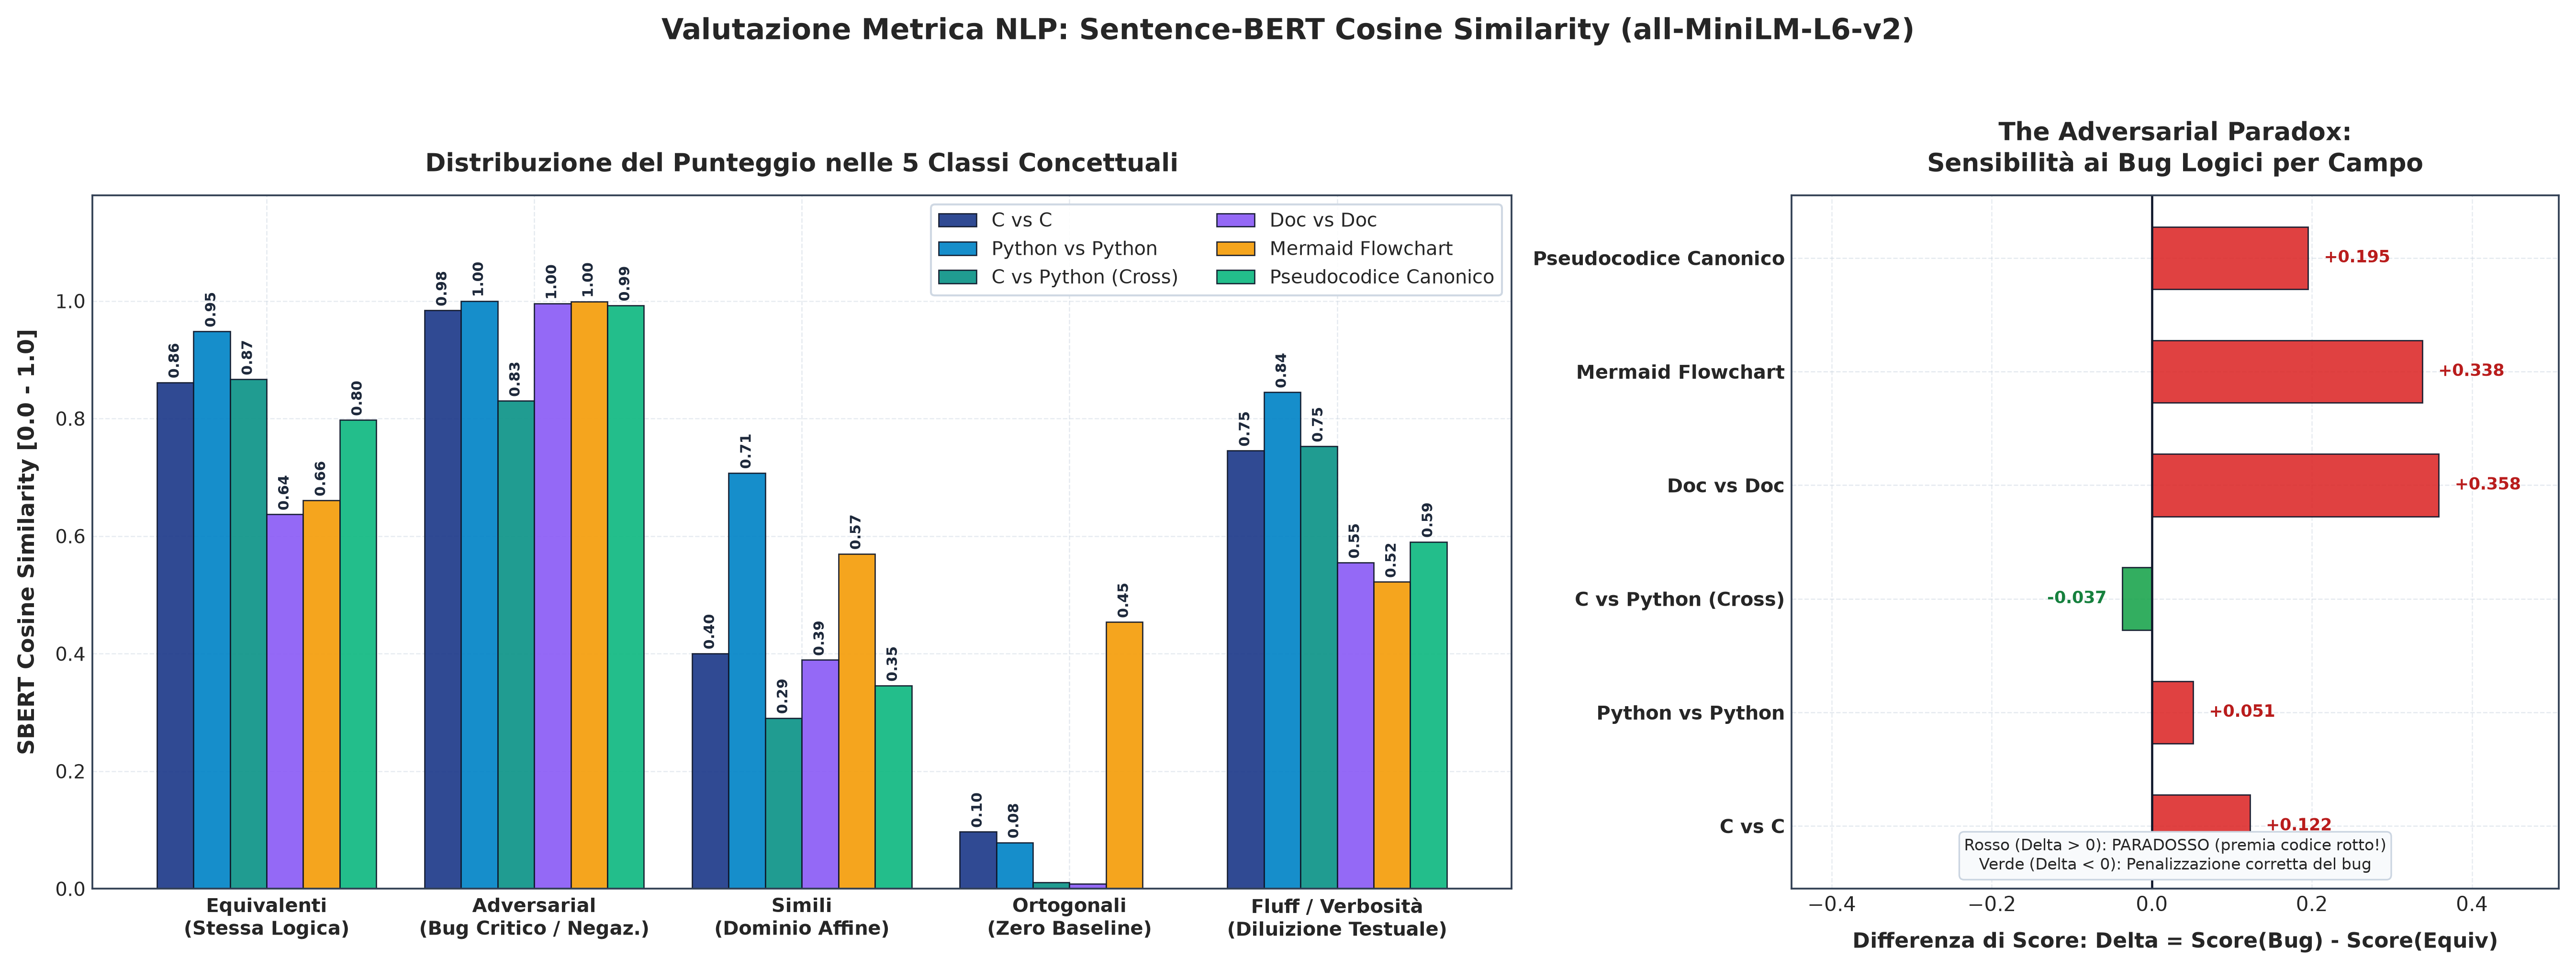
\includegraphics[width=0.85\linewidth]{figures/nlp_metric_sbert.png}
    \caption{Distribuzione dei punteggi Sentence-BERT Cosine Similarity attraverso le 5 classi semantiche nei diversi domini.}
    \label{fig:nlp_metric_sbert}
\end{figure}

\begin{itemize}[leftmargin=*, label=\textbullet]
    \item \textbf{Obiettivo Primario}: SBERT \cite{reimers_sentence-bert_2019} è stato ideato per produrre embedding densi globali di frasi o paragrafi in linguaggio naturale mediante reti siamesi a tripla loss, consentendo il confronto rapido di similarità tramite coseno tra vettori aggregati (\emph{mean pooling}).
    \item \textbf{Comportamento su Linguaggio Naturale (Doc vs Doc)}: SBERT dimostra una notevole escursione dinamica sul testo naturale puro. Come evidenziato in \Cref{fig:nlp_metric_sbert}, su testi ortogonali (\emph{TLS Socket vs Determinante}) il punteggio scende a un rassicurante $\mathbf{0.0086}$, mentre sulle parafrasi legittime attesta un valore medio di $\mathbf{0.6369}$, riflettendo la vicinanza semantica dei concetti espressi pur con lessico alternativo.
    \item \textbf{Perché 'fa fatica' sul Codice Sorgente (C vs C)}: Quando SBERT viene applicato direttamente al codice C, il meccanismo di tokenizzazione WordPiece (tarato sul corpus Wikipedia/BookCorpus) frammenta identificatori tecnici compositi (es. \texttt{sdsavail}, \texttt{cJSON\_ArrayForEach}) in una moltitudine di sottoparole prive di significato autonomo. Inoltre, il \emph{mean pooling} su tutti i token comprime l'intero flusso di controllo in un singolo vettore di 384 dimensioni. Questo provoca due distorsioni simmetriche: da un lato la totale cecità ad alterazioni di un singolo carattere sintattico fondamentale (il caso \emph{ADVERSARIAL} in C assegna un ingiustificato $\mathbf{0.9841}$ tra Minimo e Massimo), dall'altro una penalizzazione eccessiva sul codice verbose (\emph{FLUFF\_VERBOSITY} a $0.7455$), dove l'aggiunta di righe accessorie di log sposta il centroide del pooling pur mantenendo intatta la computazione.
\end{itemize}

\subsubsection{BERTScore F1}
\label{subsubsec:analisi_bertscore}

\begin{figure}[htbp]
    \centering
    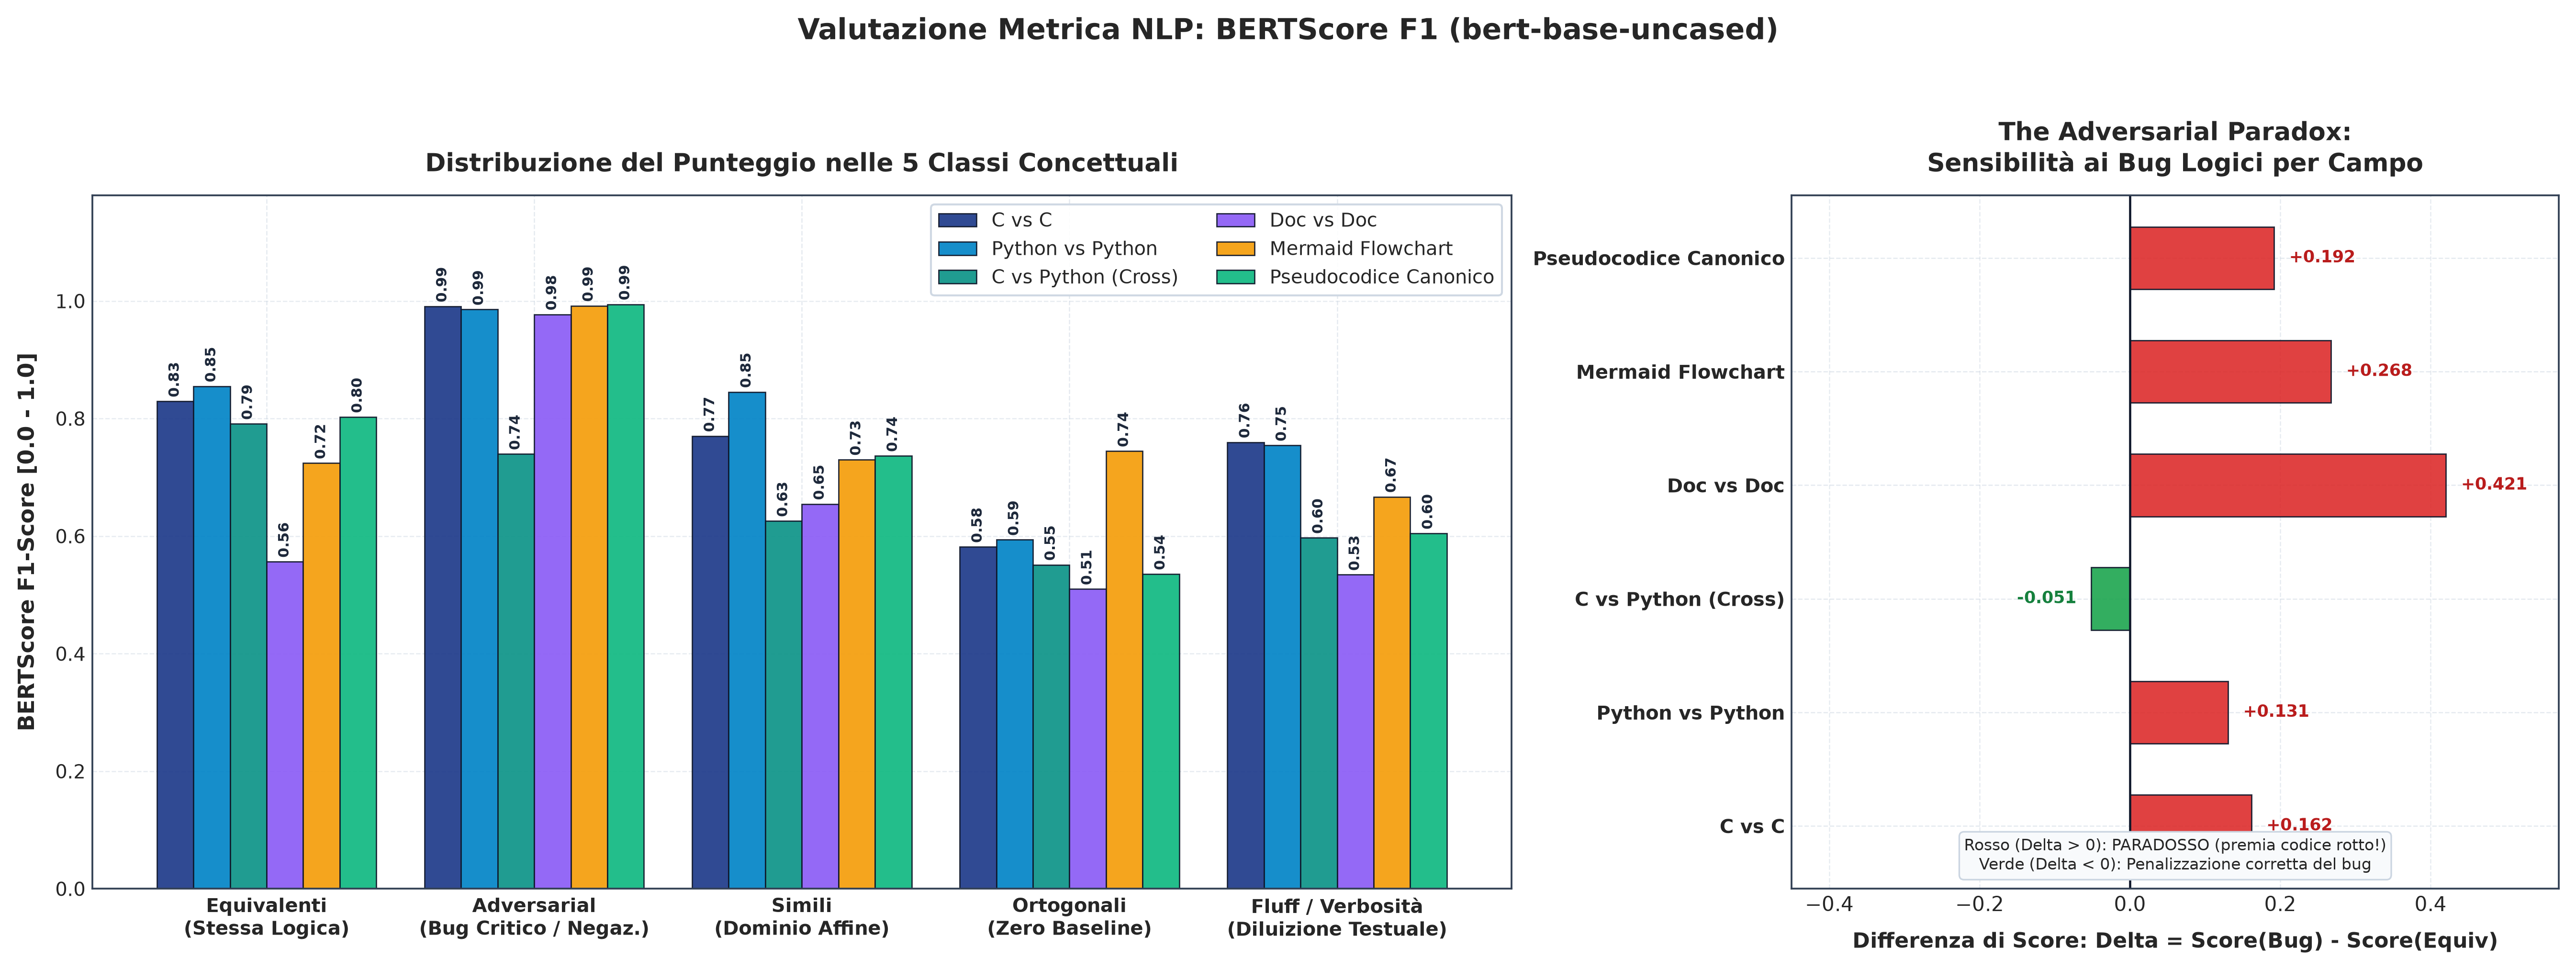
\includegraphics[width=0.85\linewidth]{figures/nlp_metric_bertscore_f1.png}
    \caption{Distribuzione dell'indicatore BERTScore F1 attraverso le 5 classi semantiche nei diversi domini.}
    \label{fig:nlp_metric_bertscore}
\end{figure}

\begin{itemize}[leftmargin=*, label=\textbullet]
    \item \textbf{Obiettivo Primario}: BERTScore \cite{zhang_bertscore_2020} è stato concepito per quantificare la similarità tra enunciati in linguaggio naturale allineando in modo greedy ciascun token dell'ipotesi al token semanticamente più affine del riferimento, sfruttando gli embedding contestuali generati dagli strati intermedi di BERT.
    \item \textbf{Comportamento su Linguaggio Naturale (Doc vs Doc)}: BERTScore cattura efficacemente l'allineamento dei singoli termini parafrasati ($F_1 = 0.5565$). Tuttavia, la sua metrica è afflitta dal noto fenomeno della \emph{compressione dinamica}: sui casi ortogonali non scende mai al di sotto di $0.5098$ (e $0.5816$ su C vs C), creando un'illusione di similarità parziale anche in assenza di qualsiasi correlazione logica.
    \item \textbf{Perché 'fa fatica' sul Codice Sorgente (C vs C)}: In una funzione C, la semantica dipende in modo stringente dalle relazioni topologiche tra variabili, operatori relazionali e ambiti di visibilità (\emph{scope}). L'allineamento greedy di BERTScore seleziona per ogni token la massima similarità coseno nell'intera sequenza di riferimento, \textbf{ignorando del tutto la posizione strutturale e l'ordine sequenziale}. Di conseguenza:
    \begin{enumerate}
        \item Su coppie avversarie (\emph{ADVERSARIAL} C vs C), BERTScore tocca l'inaccettabile punteggio di $\mathbf{0.9909}$, poiché ogni identificatore di variabile e parola chiave \texttt{if}, \texttt{int}, \texttt{return} trova una corrispondenza esatta di similarità $1.0$, mentre l'operatore invertito \texttt{<} viene allineato a \texttt{>} con un coseno residuo superiore a $0.85$.
        \item Come discusso in \Cref{fig:nlp_metric_bertscore}, la scomposizione in Precision e Recall su funzioni verbose dimostra che BERTScore intercetta il rumore lessicale (caduta della Precision a $\approx 0.54$), ma rimane cieco alle mutazioni logiche puntuali.
    \end{enumerate}
\end{itemize}

\subsubsection{CodeBERTScore F1}
\label{subsubsec:analisi_codebert}

\begin{figure}[htbp]
    \centering
    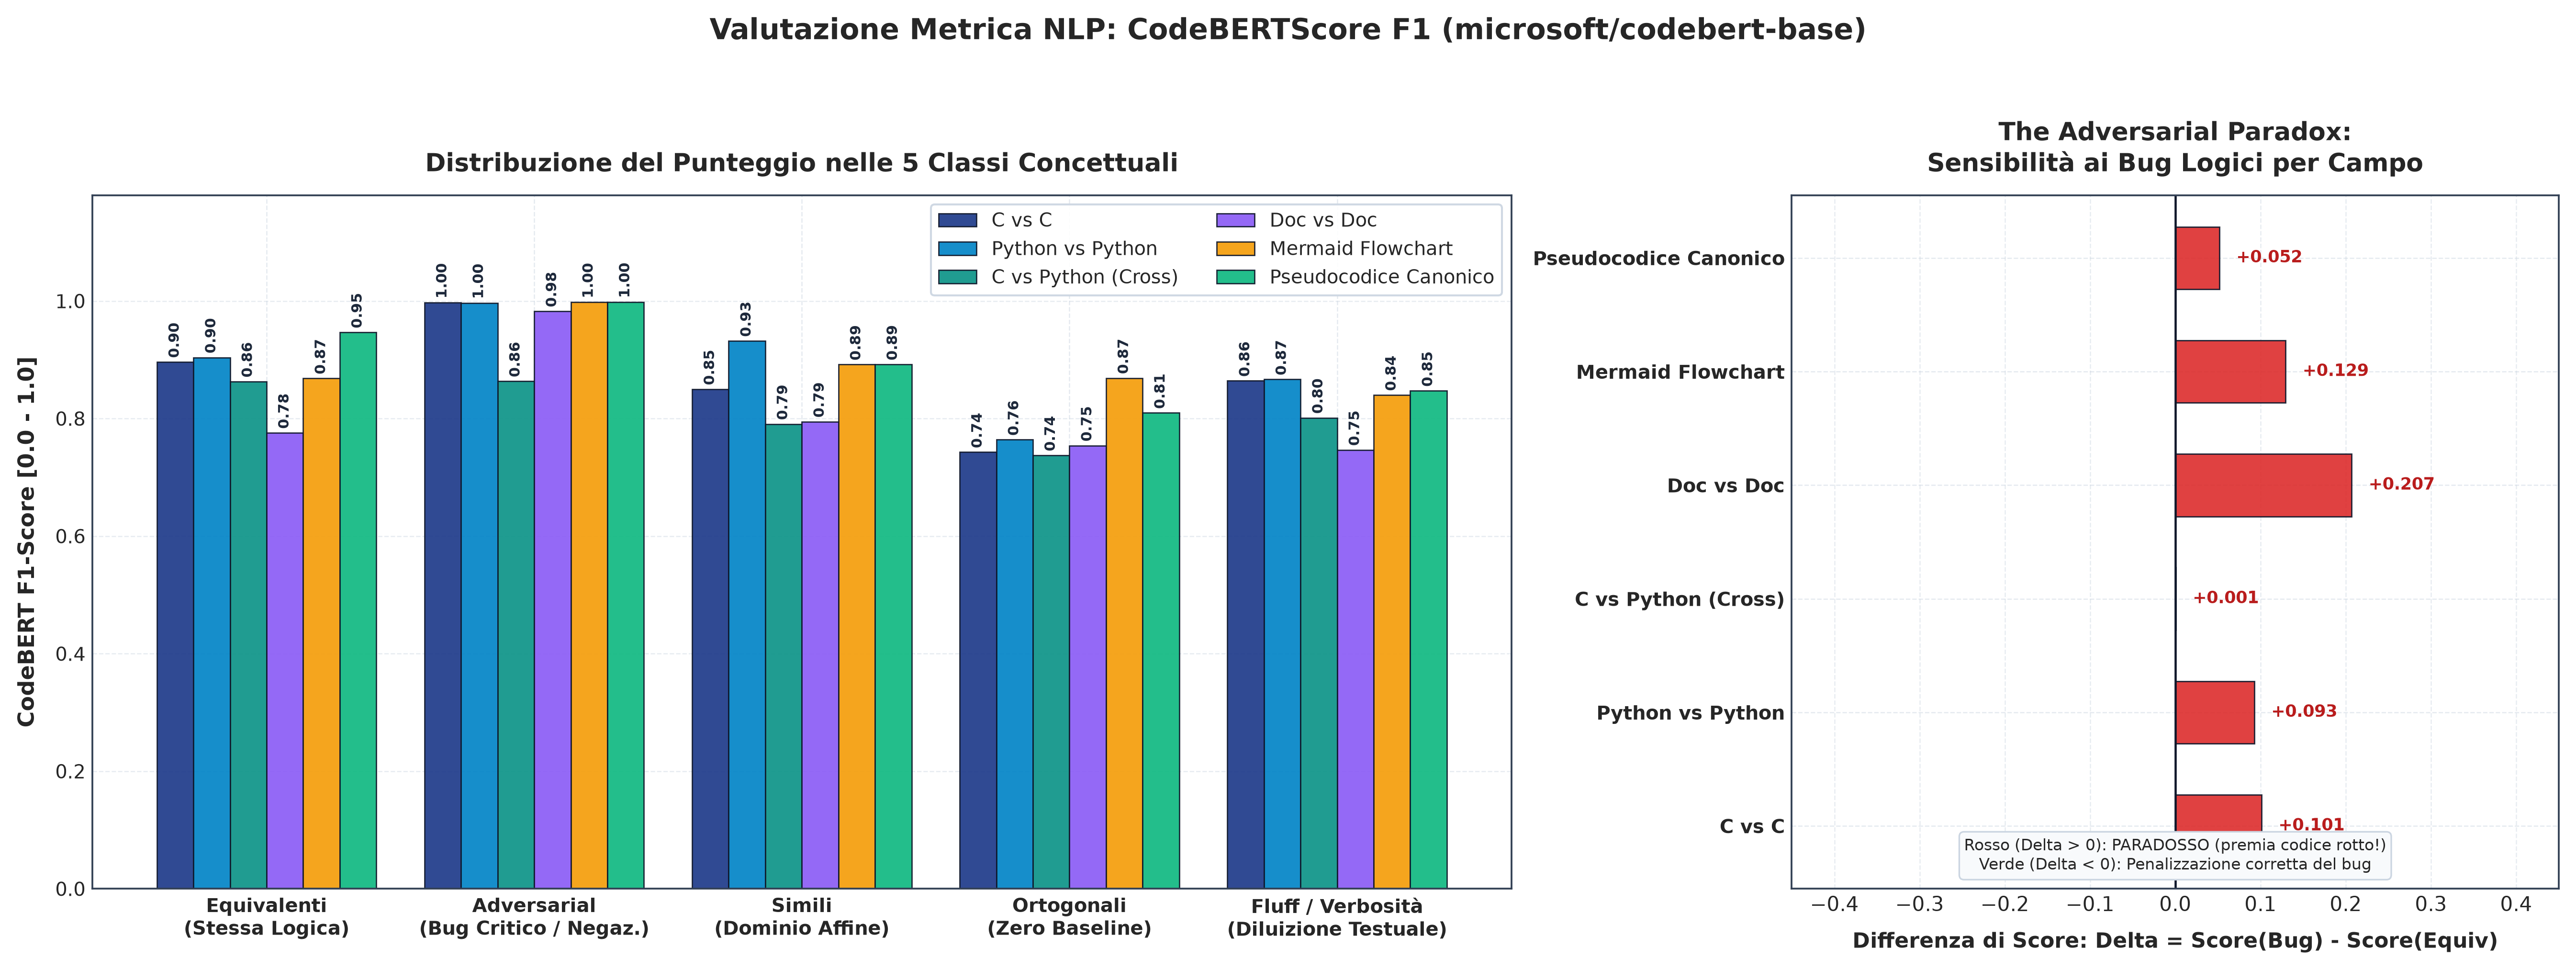
\includegraphics[width=0.85\linewidth]{figures/nlp_metric_codebert_f1.png}
    \caption{Distribuzione dell'indicatore CodeBERTScore F1 attraverso le 5 classi semantiche nei diversi domini.}
    \label{fig:nlp_metric_codebert}
\end{figure}

\begin{itemize}[leftmargin=*, label=\textbullet]
    \item \textbf{Obiettivo Primario}: CodeBERTScore \cite{zhou_codebertscore_2023} adatta il principio di BERTScore impiegando il checkpoint pre-addestrato bilingue CodeBERT \cite{feng_codebert_2020}, allenato specificamente su corpora multilingue bimodalità (Natural Language / Programming Language) comprendenti C, Java, Python, Go e documentazione associata.
    \item \textbf{Comportamento su Codice e Cross-Code}: CodeBERT si rivela la metrica più robusta nel superare le divergenze puramente sintattiche: raggiunge $F_1 = 0.8963$ su \emph{EQUIVALENT} C vs C (Fibonacci ricorsivo vs iterativo) e $0.8630$ nel confronto trans-linguistico C vs Python (\Cref{fig:nlp_metric_codebert}). Riconosce le correlazioni di flusso anche quando le strutture sintattiche divergono profondamente.
    \item \textbf{Perché 'fa fatica' e Amplifica la Cecità sui Casi Avversari}: Paradossalmente, proprio la forte componente bilingue e la spiccata invarianza alle divergenze lessicali rende CodeBERT \textbf{la metrica più pericolosa e cieca in assoluto sulle violazioni avversarie}. Sul caso \emph{ADVERSARIAL} C vs C, CodeBERT assegna il valore quasi unitario di $\mathbf{0.9974}$, e sul caso Doc vs Doc assegna $\mathbf{0.9826}$. Nello spazio vettoriale di CodeBERT, la differenza di un singolo operatore o di una parola di negazione viene assorbita dall'enorme affinità di contesto circostante, rendendo la metrica incapace di intercettare inversioni che ribaltano l'esito contrattuale del software.
\end{itemize}

\subsubsection{ROUGE-L (Longest Common Subsequence)}
\label{subsubsec:analisi_rouge_l}

\begin{figure}[htbp]
    \centering
    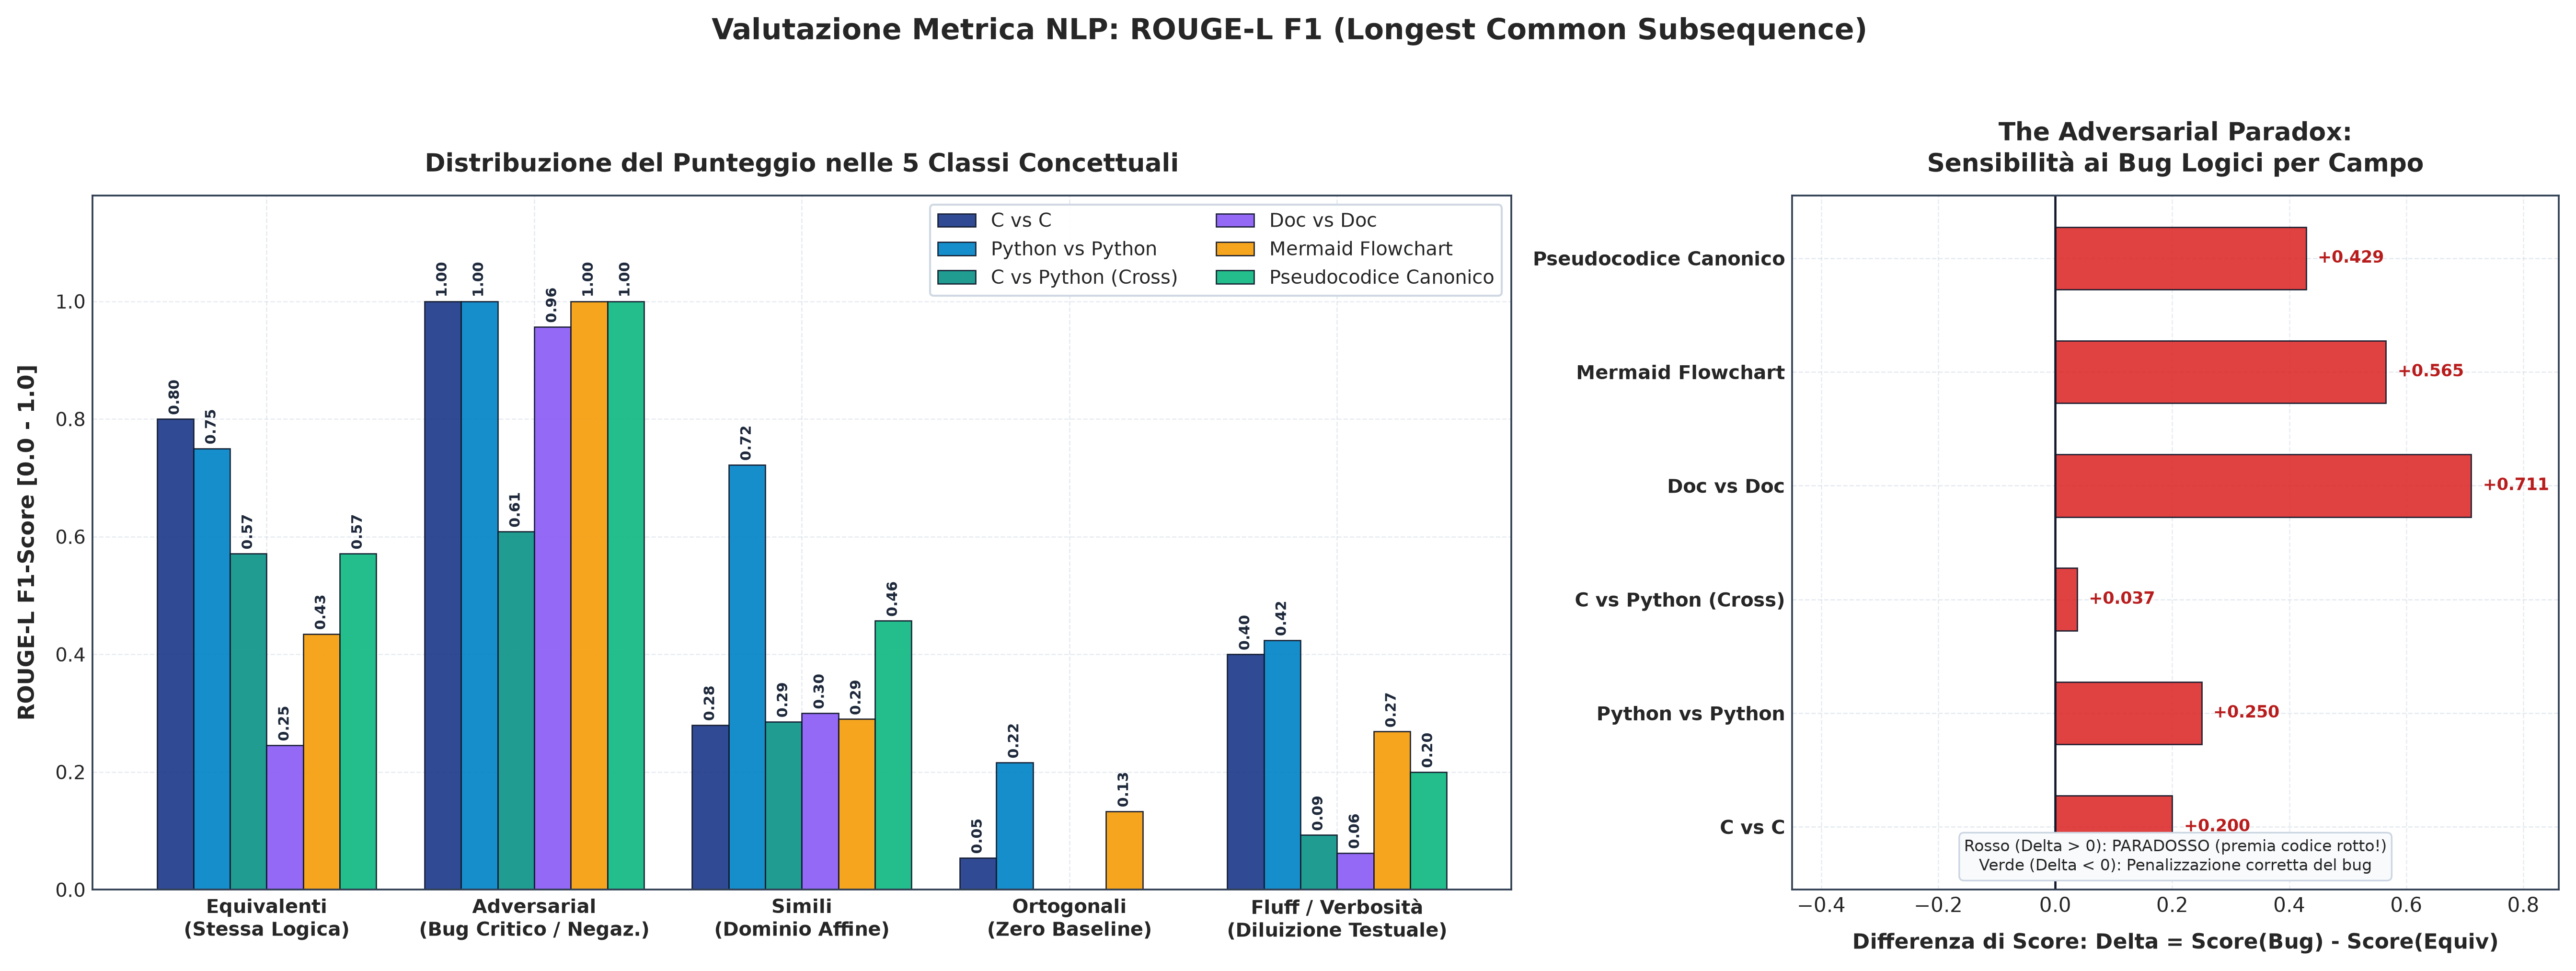
\includegraphics[width=0.85\linewidth]{figures/nlp_metric_rouge_l.png}
    \caption{Distribuzione dell'indicatore lessicale ROUGE-L attraverso le 5 classi semantiche nei diversi domini.}
    \label{fig:nlp_metric_rouge_l}
\end{figure}

\begin{itemize}[leftmargin=*, label=\textbullet]
    \item \textbf{Obiettivo Primario}: ROUGE-L \cite{lin_rouge_2004} è una metrica superficiale basata sulla più lunga sottosequenza comune di token a livello di frase, concepita originariamente per valutare la coerenza sequenziale nei sistemi di riassunto automatico.
    \item \textbf{Comportamento su Linguaggio Naturale (Doc vs Doc)}: Come mostrato in \Cref{fig:nlp_metric_rouge_l}, ROUGE-L è rigidissima di fronte a qualsiasi parafrasi lessicale: su testi perfettamente equivalenti ma espressi con vocabolario differente (\emph{EQUIVALENT} Doc vs Doc), crolla a $\mathbf{0.2456}$. Su testi ortogonali tocca lo zero assoluto ($\mathbf{0.0000}$), offrendo una perfetta discriminazione del testo privo di parole condivise.
    \item \textbf{Perché 'fa fatica' sul Codice Sorgente (C vs C)}: ROUGE-L opera come mero allineatore sequenziale privo di consapevolezza grammaticale. Sul codice C, una semplice inversione di due blocchi indipendenti di codice o la modifica dell'ordine delle dichiarazioni di variabili fa crollare la sottosequenza comune, mentre la sostituzione di \texttt{<} con \texttt{>} lascia la sequenza inalterata per il 99\% dei token, producendo un ingannevole punteggio di $\mathbf{1.0000}$ sul caso \emph{ADVERSARIAL}.
\end{itemize}

\subsubsection{TF-IDF Cosine Similarity}
\label{subsubsec:analisi_tfidf}

\begin{figure}[htbp]
    \centering
    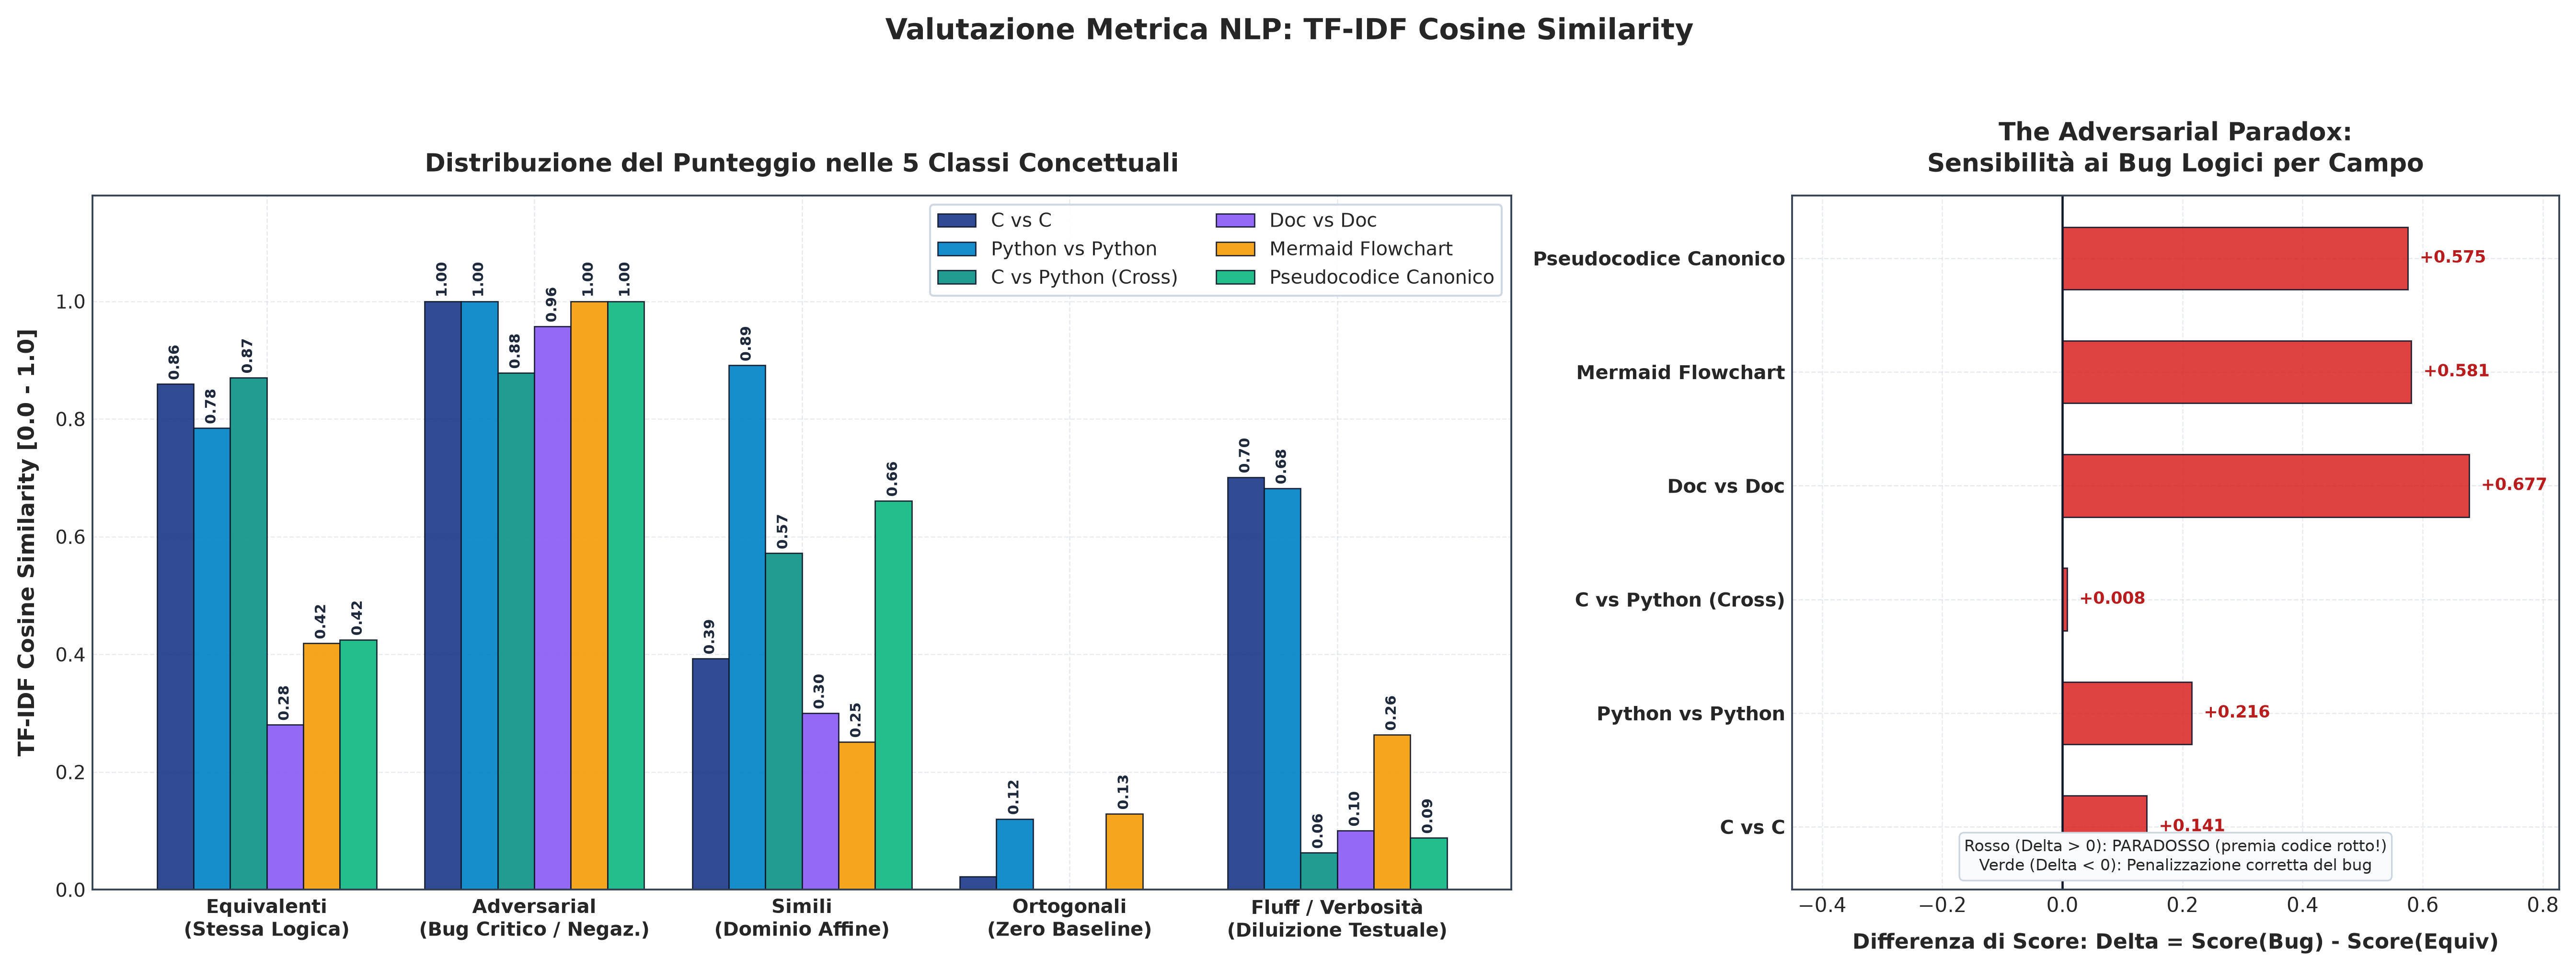
\includegraphics[width=0.85\linewidth]{figures/nlp_metric_tfidf_cosine.png}
    \caption{Distribuzione dell'indicatore statistico TF-IDF Cosine Similarity attraverso le 5 classi semantiche nei diversi domini.}
    \label{fig:nlp_metric_tfidf}
\end{figure}

\begin{itemize}[leftmargin=*, label=\textbullet]
    \item \textbf{Obiettivo Primario}: TF-IDF (Term Frequency - Inverse Document Frequency) è una metrica classica dell'Information Retrieval basata sul modello a sacco di parole (\emph{bag-of-words}), pesata per la rarità statistica dei termini all'interno del corpus.
    \item \textbf{Comportamento su Linguaggio Naturale (Doc vs Doc)}: TF-IDF discrimina in modo ineccepibile i domini ortogonali ($\mathbf{0.0000}$ su Doc vs Doc e $0.0223$ su C vs C), poiché termini specialistici di algebra lineare e di programmazione di rete non condividono vocaboli.
    \item \textbf{Perché 'fa fatica' sul Codice Sorgente (C vs C)}: Il codice sorgente possiede una sintassi ad albero fortemente strutturata dove la posizione degli identificatori ne determina il significato. Essendo TF-IDF per definizione \textbf{totalmente cieca all'ordine dei token e alla struttura gerarchica}, due funzioni che contengono gli stessi identificatori ma con ruoli scambiati (\texttt{src} in \texttt{dest} vs \texttt{dest} in \texttt{src}) ottengono un coseno identico a $1.0000$. Inoltre, sul caso \emph{ADVERSARIAL} C vs C, TF-IDF assegna un punteggio pieno di $\mathbf{1.0000}$, confermando l'incapacità di rilevare mutazioni puntuali.
\end{itemize}

\subsubsection{METEOR (Metric for Evaluation of Translation with Explicit ORdering)}
\label{subsubsec:analisi_meteor}

\begin{figure}[htbp]
    \centering
    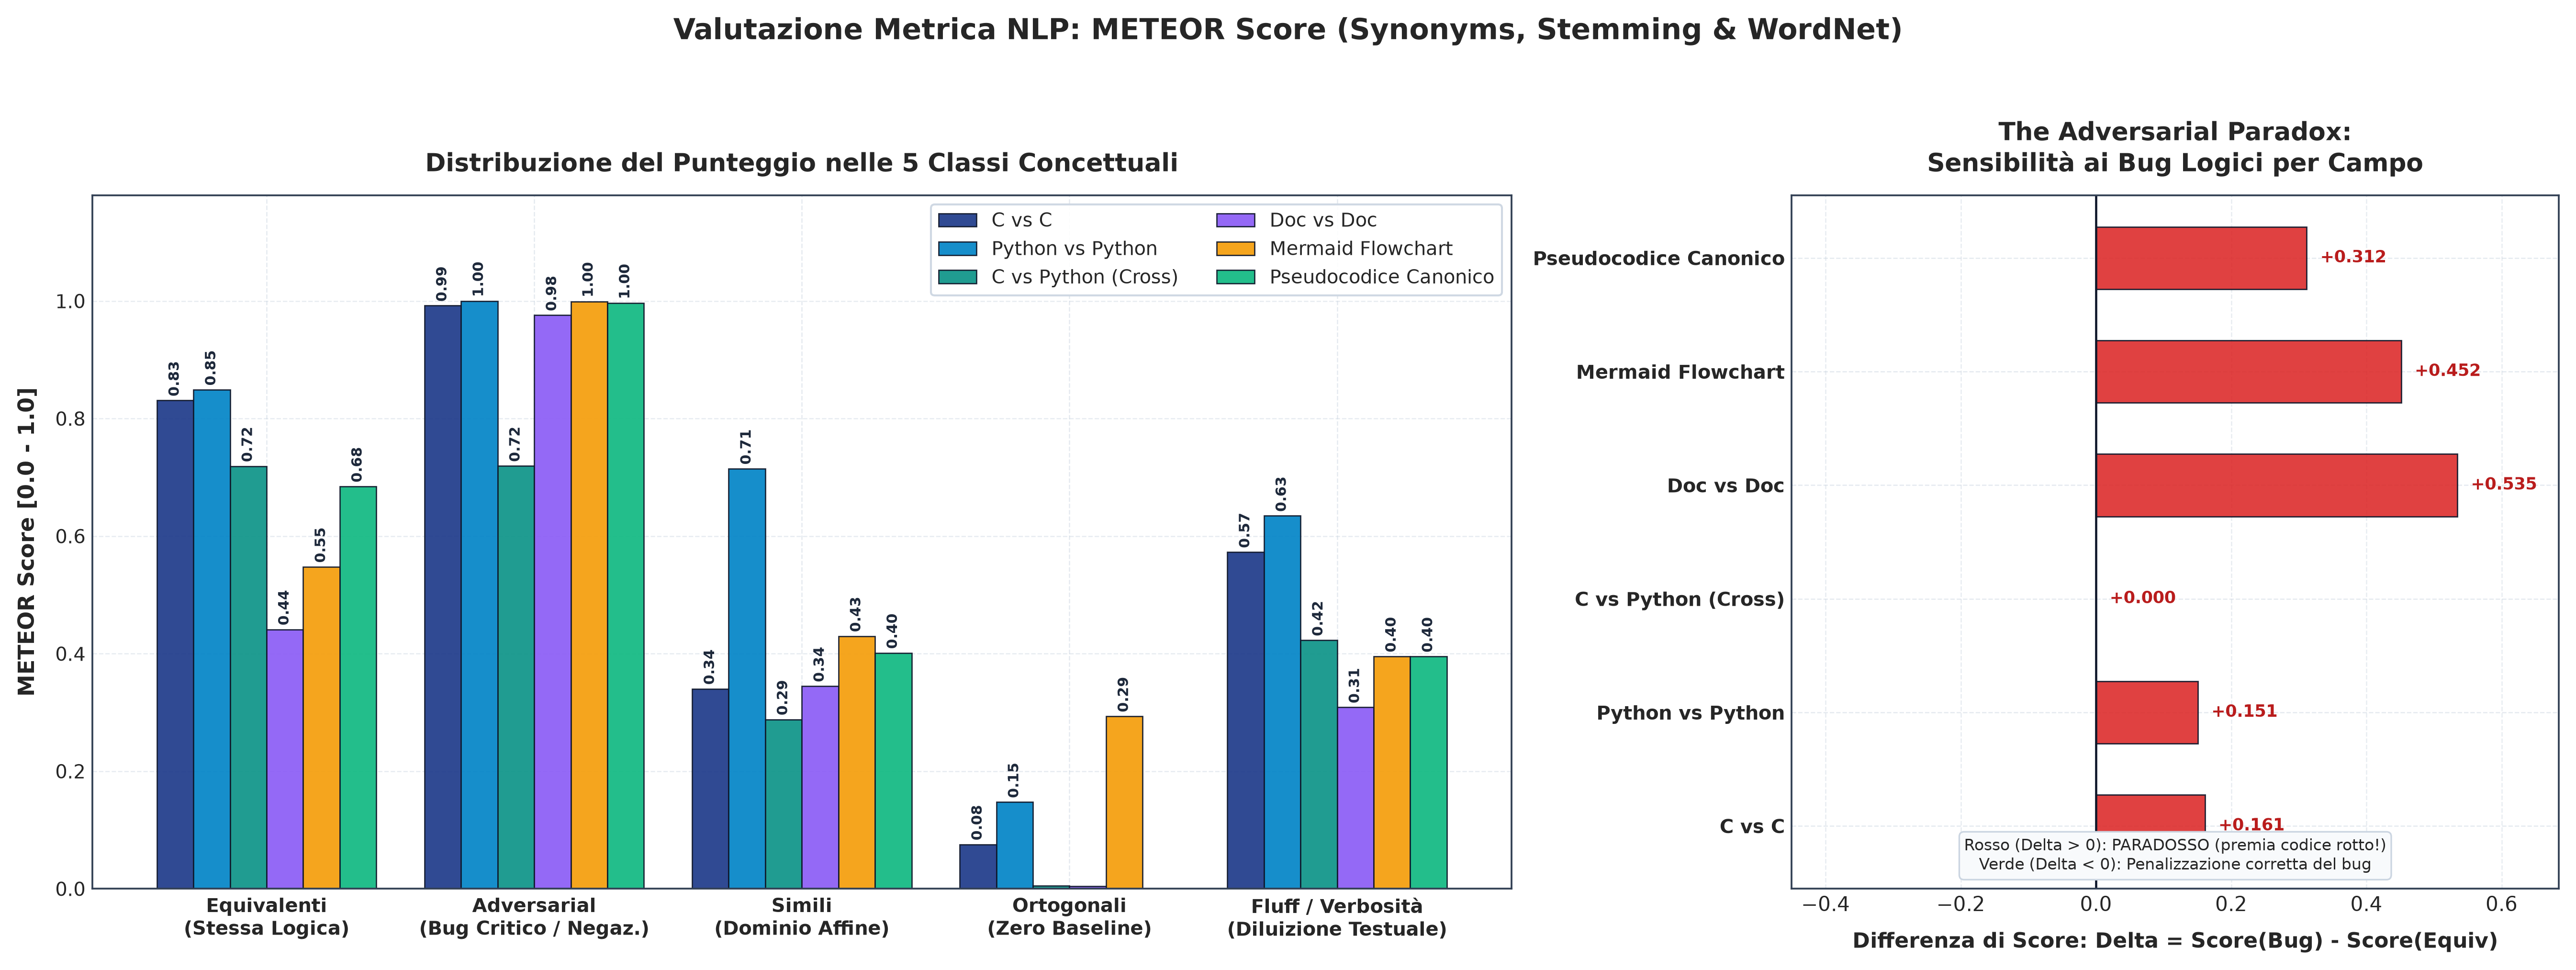
\includegraphics[width=0.85\linewidth]{figures/nlp_metric_meteor.png}
    \caption{Distribuzione dell'indicatore METEOR attraverso le 5 classi semantiche nei diversi domini.}
    \label{fig:nlp_metric_meteor}
\end{figure}

\begin{itemize}[leftmargin=*, label=\textbullet]
    \item \textbf{Obiettivo Primario}: METEOR \cite{banerjee_meteor_2005} è stata progettata per superare la rigidità di BLEU nella Machine Translation mediante una catena gerarchica di moduli di allineamento unigramma: match esatto, stemming morfologico (algoritmo di Porter) e sinonimia lessicale derivata da WordNet, integrati da una penalità di frammentazione (\emph{chunk penalty}).
    \item \textbf{Comportamento su Linguaggio Naturale (Doc vs Doc)}: Su documentazione tecnica, il modulo dei sinonimi permette a METEOR di gestire variazioni verbali legittime (es. \emph{allocate} / \emph{create}, \emph{retrieve} / \emph{fetch}), attestandosi a $0.4413$ su parafrasi ed eliminando quasi integralmente i falsi positivi su testi ortogonali ($0.0043$).
    \item \textbf{Perché 'fa fatica' sul Codice Sorgente (C vs C)}: Gli identificatori del codice C/C++ seguono convenzioni morfologiche artificiali (\texttt{snake\_case}, \texttt{camelCase}) e abbreviazioni arbitrarie (\texttt{ptr}, \texttt{idx}, \texttt{ctx}, \texttt{buf}) che non trovano alcuna corrispondenza nei synset di WordNet né nelle regole di stemming della lingua inglese. Inoltre, il modulo di match unigramma di METEOR tratta gli operatori di confronto e di assegnamento come punteggiatura secondaria: ne consegue che sul caso \emph{ADVERSARIAL} C vs C la penalità di frammentazione è trascurabile, producendo un punteggio errato di $\mathbf{0.9920}$ (\Cref{fig:nlp_metric_meteor}).
\end{itemize}

\subsubsection{BLEURT (Bilingual Evaluation Understudy with Representations from Transformers)}
\label{subsubsec:analisi_bleurt}

\begin{figure}[htbp]
    \centering
    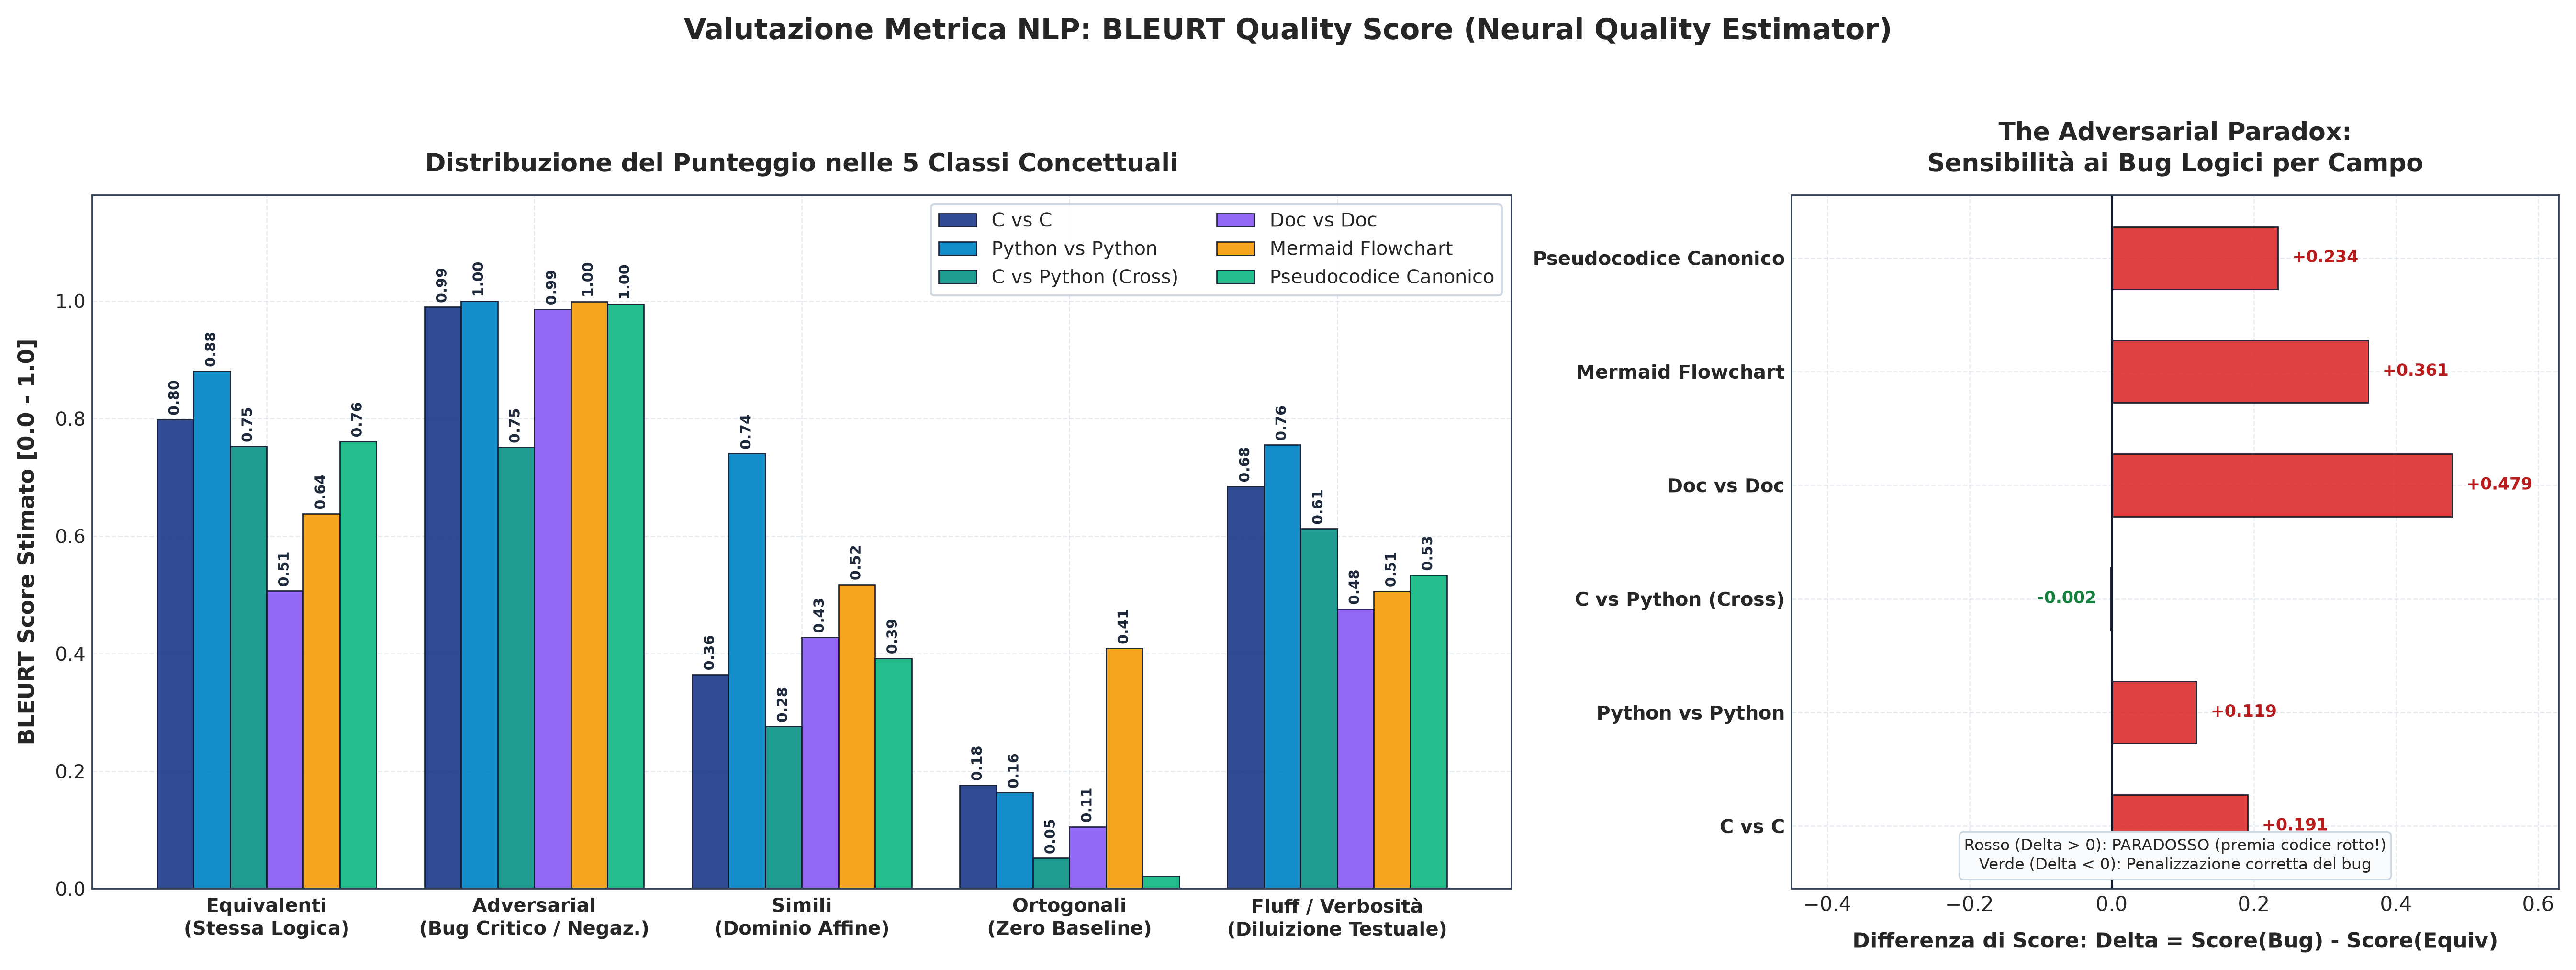
\includegraphics[width=0.85\linewidth]{figures/nlp_metric_bleurt.png}
    \caption{Distribuzione dell'indicatore BLEURT attraverso le 5 classi semantiche nei diversi domini.}
    \label{fig:nlp_metric_bleurt}
\end{figure}

\begin{itemize}[leftmargin=*, label=\textbullet]
    \item \textbf{Obiettivo Primario}: BLEURT \cite{sellam_bleurt_2020} è una metrica di regressione neurale basata su BERT, pre-addestrata su milioni di coppie di frasi sinteticamente perturbate e fine-tunata su giudizi umani di qualità della traduzione automatica (WMT Metrics).
    \item \textbf{Comportamento su Linguaggio Naturale (Doc vs Doc)}: Grazie all'addestramento su coppie supervisionate, BLEURT esibisce una buona correlazione con l'aderenza stilistica su testi in lingua naturale (\Cref{fig:nlp_metric_bleurt}), posizionandosi a $0.5071$ su parafrasi e scendendo a $0.1056$ su testi ortogonali.
    \item \textbf{Perché 'fa fatica' sul Codice Sorgente (C vs C)}: La funzione di perdita di regressione di BLEURT è stata calibrata su valutazioni umane di fluidità e adeguatezza di traduzioni narrative. Quando è alimentata con token sintattici imperativi del C (\texttt{typedef}, \texttt{sizeof}, dereferenziazione di puntatori \texttt{*ptr++}), la metrica entra in una regione distributiva completamente \emph{out-of-distribution}. Sul caso \emph{ADVERSARIAL} C vs C, BLEURT restituisce un fuorviante $\mathbf{0.9897}$, dimostrando che il pre-addestramento su perturbazioni del linguaggio naturale non conferisce alcuna robustezza logica nel dominio software.
\end{itemize}

---

\section{Validazione Empirica delle Metriche Avanzate di Livello II, III e IV}
\label{sec:validazione_metriche_avanzate}

I limiti intrinseci e strutturali evidenziati nell'analisi delle metriche di NLP testuale impongono l'adozione del framework multi-livello descritto in \Cref{chap:metriche}. In questa sezione vengono analizzati i dati empirici raccolti sulle metriche avanzate: la copertura formale dei contratti (\emph{Concept Checklist Score}), la valutazione semantica guidata da rubriche (\emph{LLM-as-a-Judge}), l'esecuzione a scatola nera (\emph{Round-Trip Differential Testing}) e l'utilità nel reperimento semantico (\emph{Code Retrieval MRR}).

\begin{figure}[htbp]
    \centering
    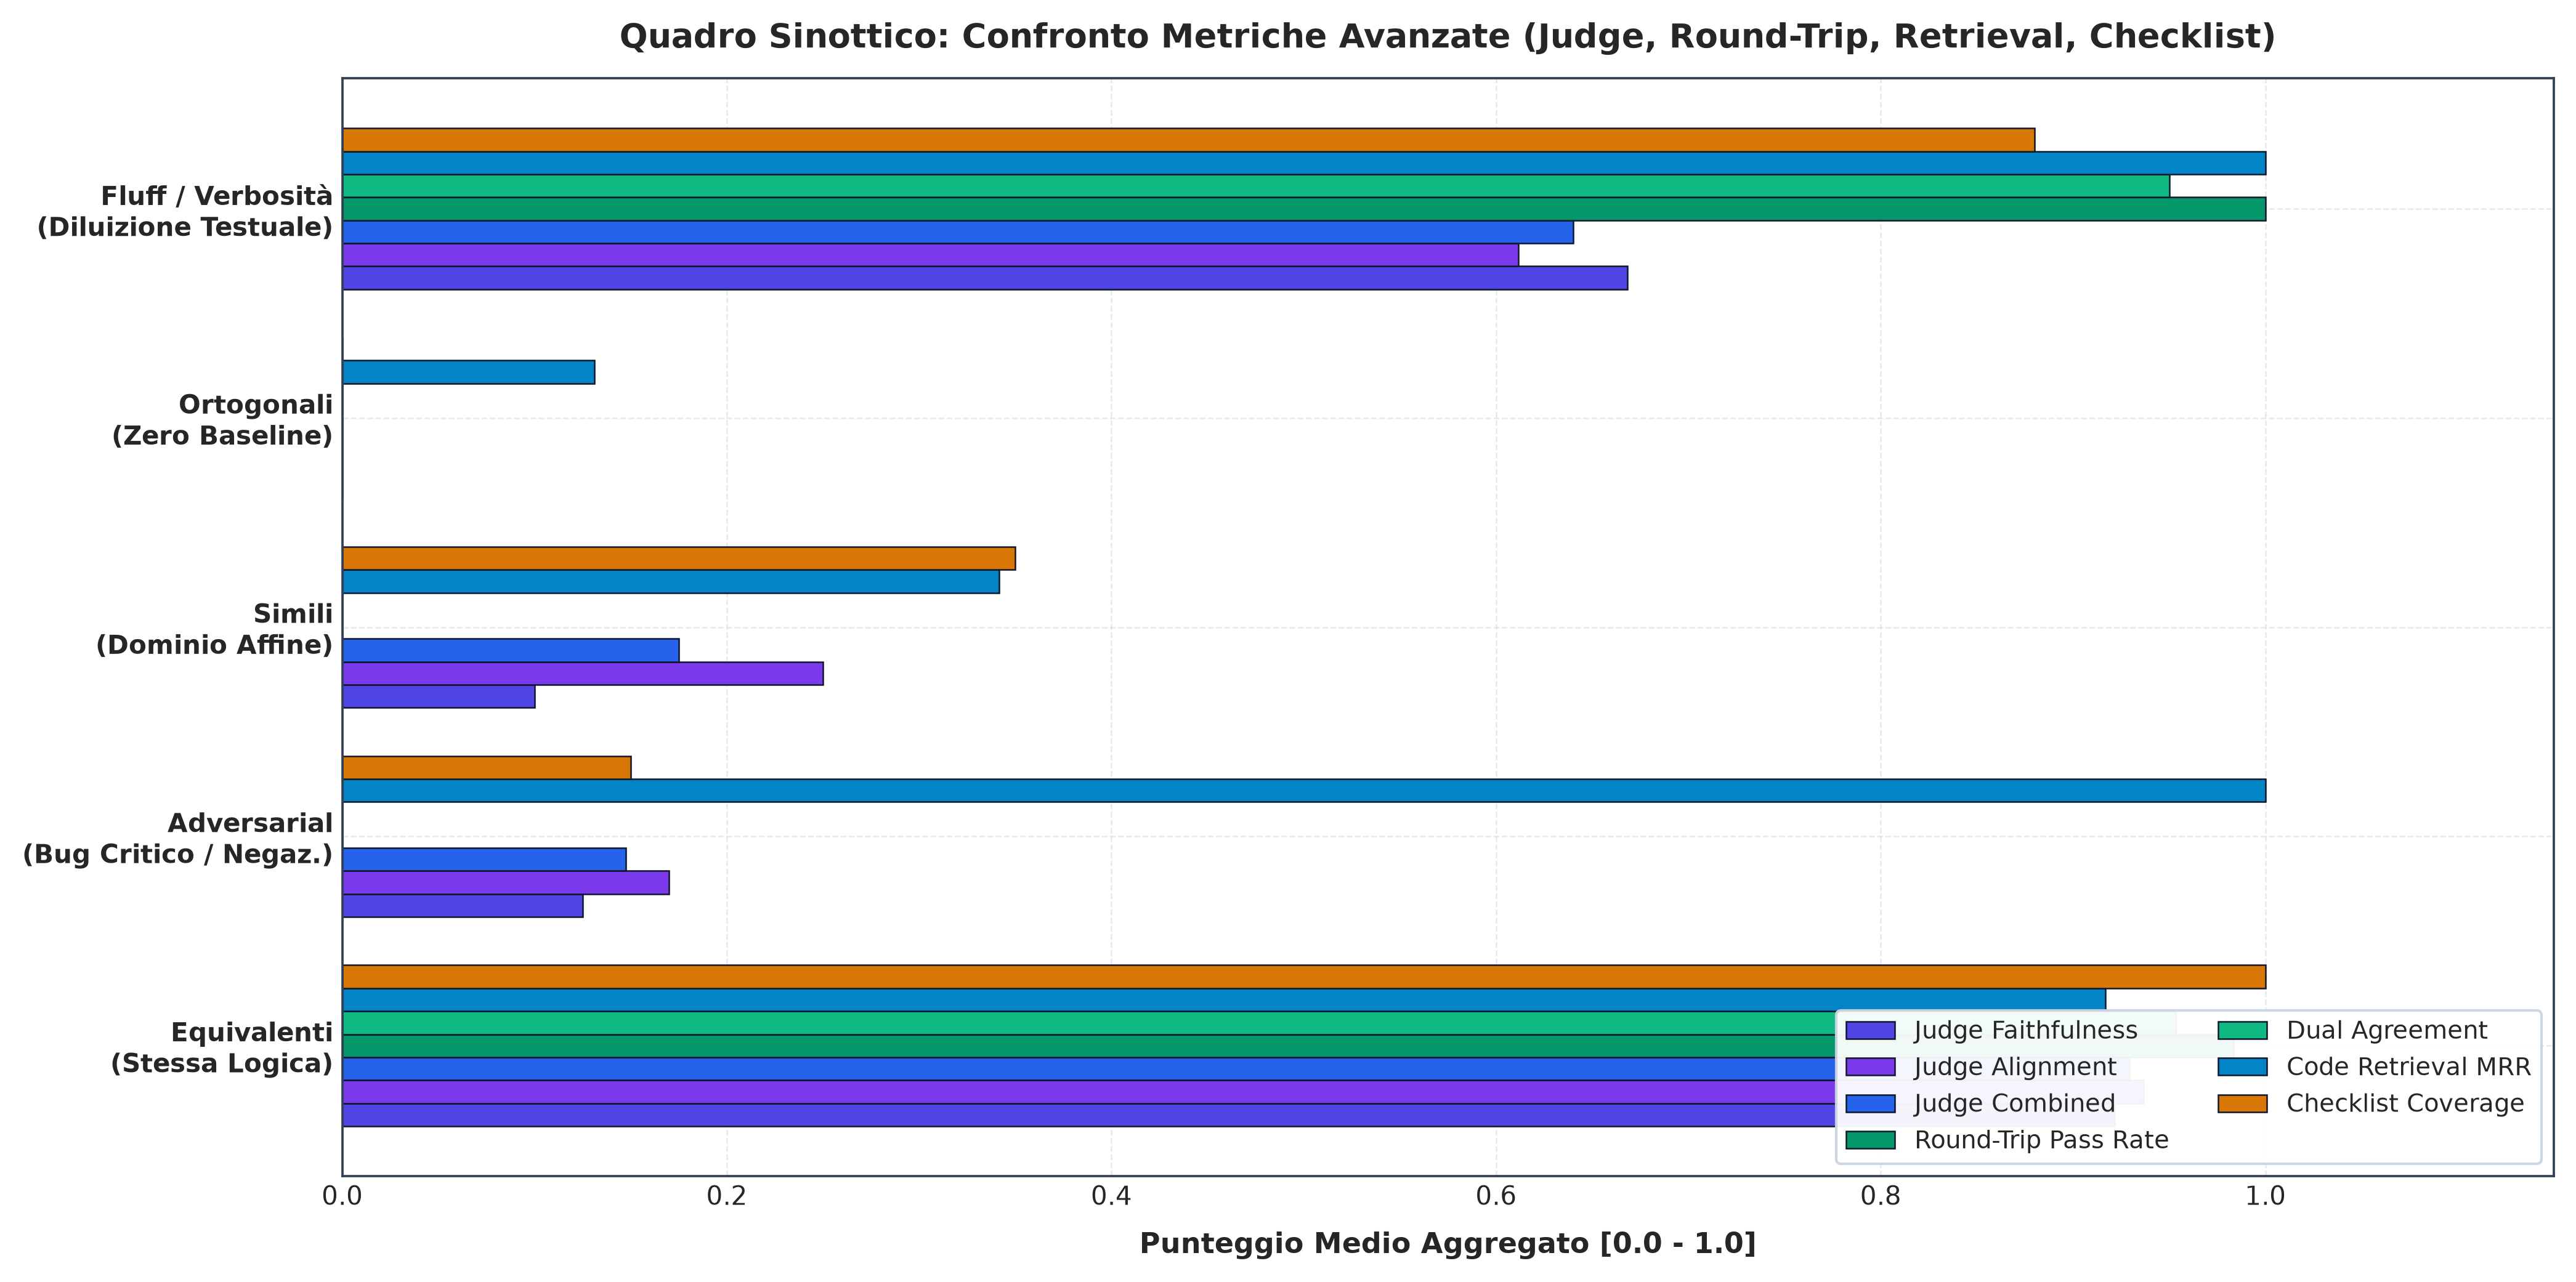
\includegraphics[width=0.95\linewidth]{figures/advanced_metric_overview_all_classes.png}
    \caption{Panoramica aggregata delle metriche avanzate (LLM-Judge, Round-Trip Pass Rate, Dual Agreement, Retrieval MRR e Concept Checklist) attraverso le 5 classi semantiche.}
    \label{fig:advanced_metric_overview}
\end{figure}

I risultati sperimentali sono presentati nella panoramica globale di \Cref{fig:advanced_metric_overview} e dettagliati in \Cref{tab:advanced_metrics_summary}.

\begin{table}[htbp]
\centering
\scriptsize
\setlength{\tabcolsep}{3pt}
\caption{Risultati comparativi delle metriche avanzate sui domini C vs C, Doc vs Doc e media globale.}
\label{tab:advanced_metrics_summary}
\begin{tabular}{llccccc}
\toprule
\textbf{Classe Semantica} & \textbf{Dominio} & \textbf{Judge Faith.} & \textbf{Judge Align.} & \textbf{RT Pass Rate} & \textbf{Dual Agree} & \textbf{Checklist} \\
\midrule
\multirow{3}{*}{\textbf{EQUIVALENT}} 
  & C vs C & 0.950 & 0.950 & 1.000 & 1.000 & 1.000 \\
  & Doc vs Doc & 0.920 & 0.960 & 1.000 & 0.950 & 1.000 \\
  & \emph{Media Globale} & \emph{0.922} & \emph{0.937} & \emph{0.983} & \emph{0.953} & \emph{1.000} \\
\midrule
\multirow{3}{*}{\textbf{ADVERSARIAL}} 
  & C vs C & \textbf{0.150} & \textbf{0.200} & \textbf{0.000} & \textbf{0.000} & \textbf{0.150} \\
  & Doc vs Doc & \textbf{0.050} & \textbf{0.100} & \textbf{0.000} & \textbf{0.000} & \textbf{0.150} \\
  & \emph{Media Globale} & \textbf{\emph{0.125}} & \textbf{\emph{0.170}} & \textbf{\emph{0.000}} & \textbf{\emph{0.000}} & \textbf{\emph{0.150}} \\
\midrule
\multirow{3}{*}{\textbf{DOMAIN\_SIMILAR}} 
  & C vs C & 0.100 & 0.250 & 0.000 & 0.000 & 0.350 \\
  & Doc vs Doc & 0.100 & 0.250 & 0.000 & 0.000 & 0.350 \\
  & \emph{Media Globale} & \emph{0.100} & \emph{0.250} & \emph{0.000} & \emph{0.000} & \emph{0.350} \\
\midrule
\multirow{3}{*}{\textbf{ORTHOGONAL}} 
  & C vs C & 0.000 & 0.000 & 0.000 & 0.000 & 0.000 \\
  & Doc vs Doc & 0.000 & 0.000 & 0.000 & 0.000 & 0.000 \\
  & \emph{Media Globale} & \emph{0.000} & \emph{0.000} & \emph{0.000} & \emph{0.000} & \emph{0.000} \\
\midrule
\multirow{3}{*}{\textbf{FLUFF\_VERBOSITY}} 
  & C vs C & 0.700 & 0.650 & 1.000 & 0.950 & 0.880 \\
  & Doc vs Doc & 0.600 & 0.550 & 1.000 & 0.950 & 0.880 \\
  & \emph{Media Globale} & \emph{0.668} & \emph{0.612} & \emph{1.000} & \emph{0.950} & \emph{0.880} \\
\bottomrule
\end{tabular}
\end{table}

\subsection{Concept Checklist Score}
\label{subsec:analisi_checklist}

\begin{figure}[htbp]
    \centering
    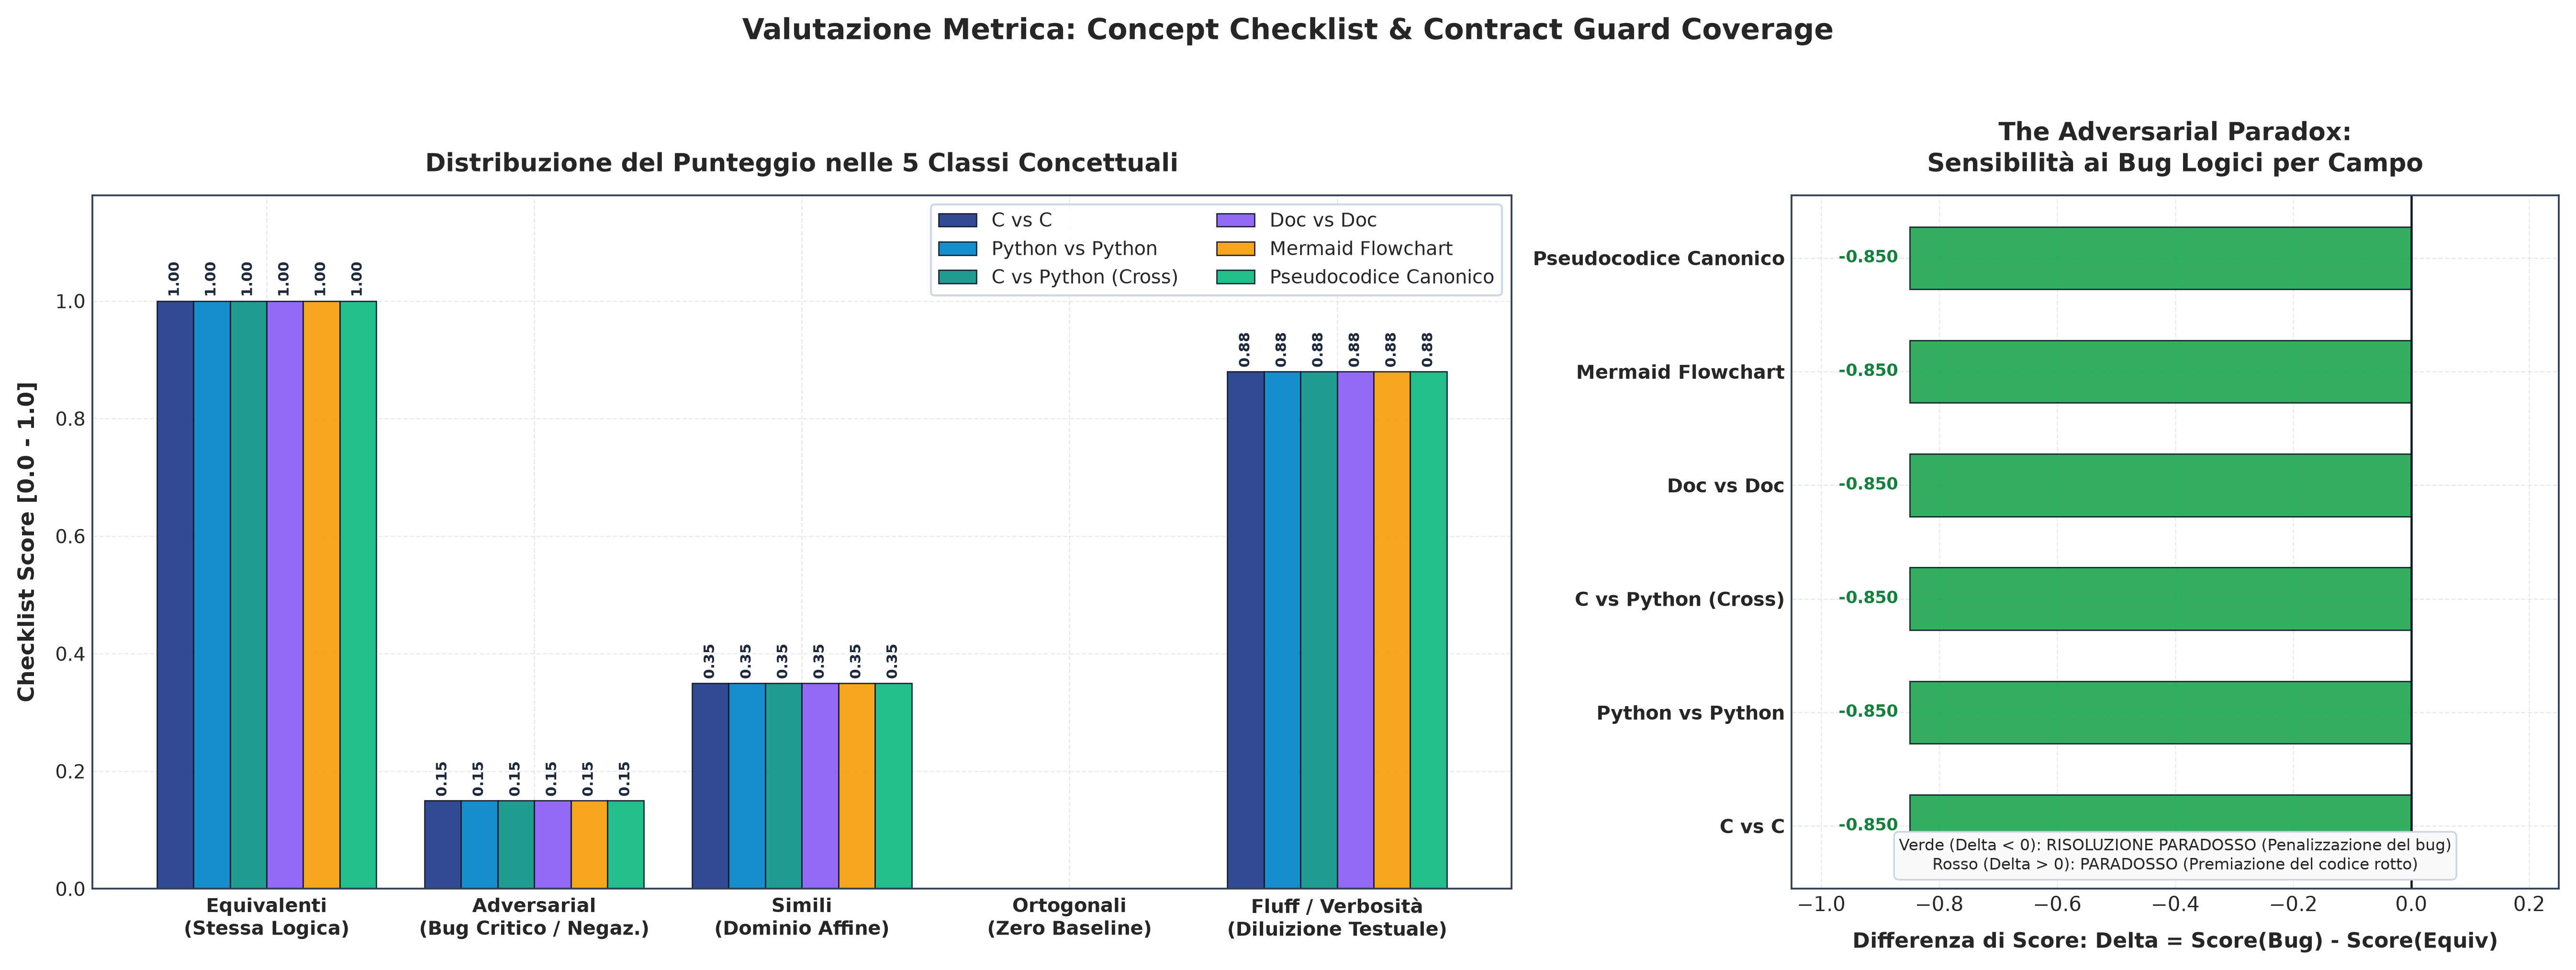
\includegraphics[width=0.85\linewidth]{figures/concept_checklist_score.png}
    \caption{Distribuzione dell'indicatore Concept Checklist Score attraverso le 5 classi semantiche nei diversi domini.}
    \label{fig:concept_checklist}
\end{figure}

La metrica \emph{Concept Checklist Score} valuta la presenza e la conformità esplicita di clausole contrattuali critiche nel testo Doxygen (\Cref{fig:concept_checklist}):
\begin{itemize}
    \item \textbf{Robustezza e Risultati}: Sui casi equivalenti e completi, la checklist rileva la totalità dei contratti essenziali (allocazione memoria, gestione puntatori nulli, codici di ritorno), attestandosi a un perfetto $\mathbf{1.0000}$. Nei casi di verbosità (\emph{FLUFF\_VERBOSITY}), il punteggio si attesta a $\mathbf{0.8800}$, riconoscendo che la sostanza contrattuale è stata preservata nonostante la prolissità.
    \item \textbf{Sensibilità Avversaria}: Quando un vincolo di ownership o precondizione viene ribaltato (\emph{ADVERSARIAL}), il punteggio della checklist crolla a $\mathbf{0.1500}$. A differenza delle metriche NLP dense che registravano $\approx 0.98$, la checklist intercetta la violazione del pattern atteso, confermandosi un gate di qualità indispensabile a monte delle pipeline di rilascio.
\end{itemize}

\subsection{LLM-as-a-Judge: Disaccoppiamento tra Faithfulness e Alignment}
\label{subsec:analisi_llm_judge}

\begin{figure}[htbp]
    \centering
    \begin{subfigure}[b]{0.32\textwidth}
        \centering
        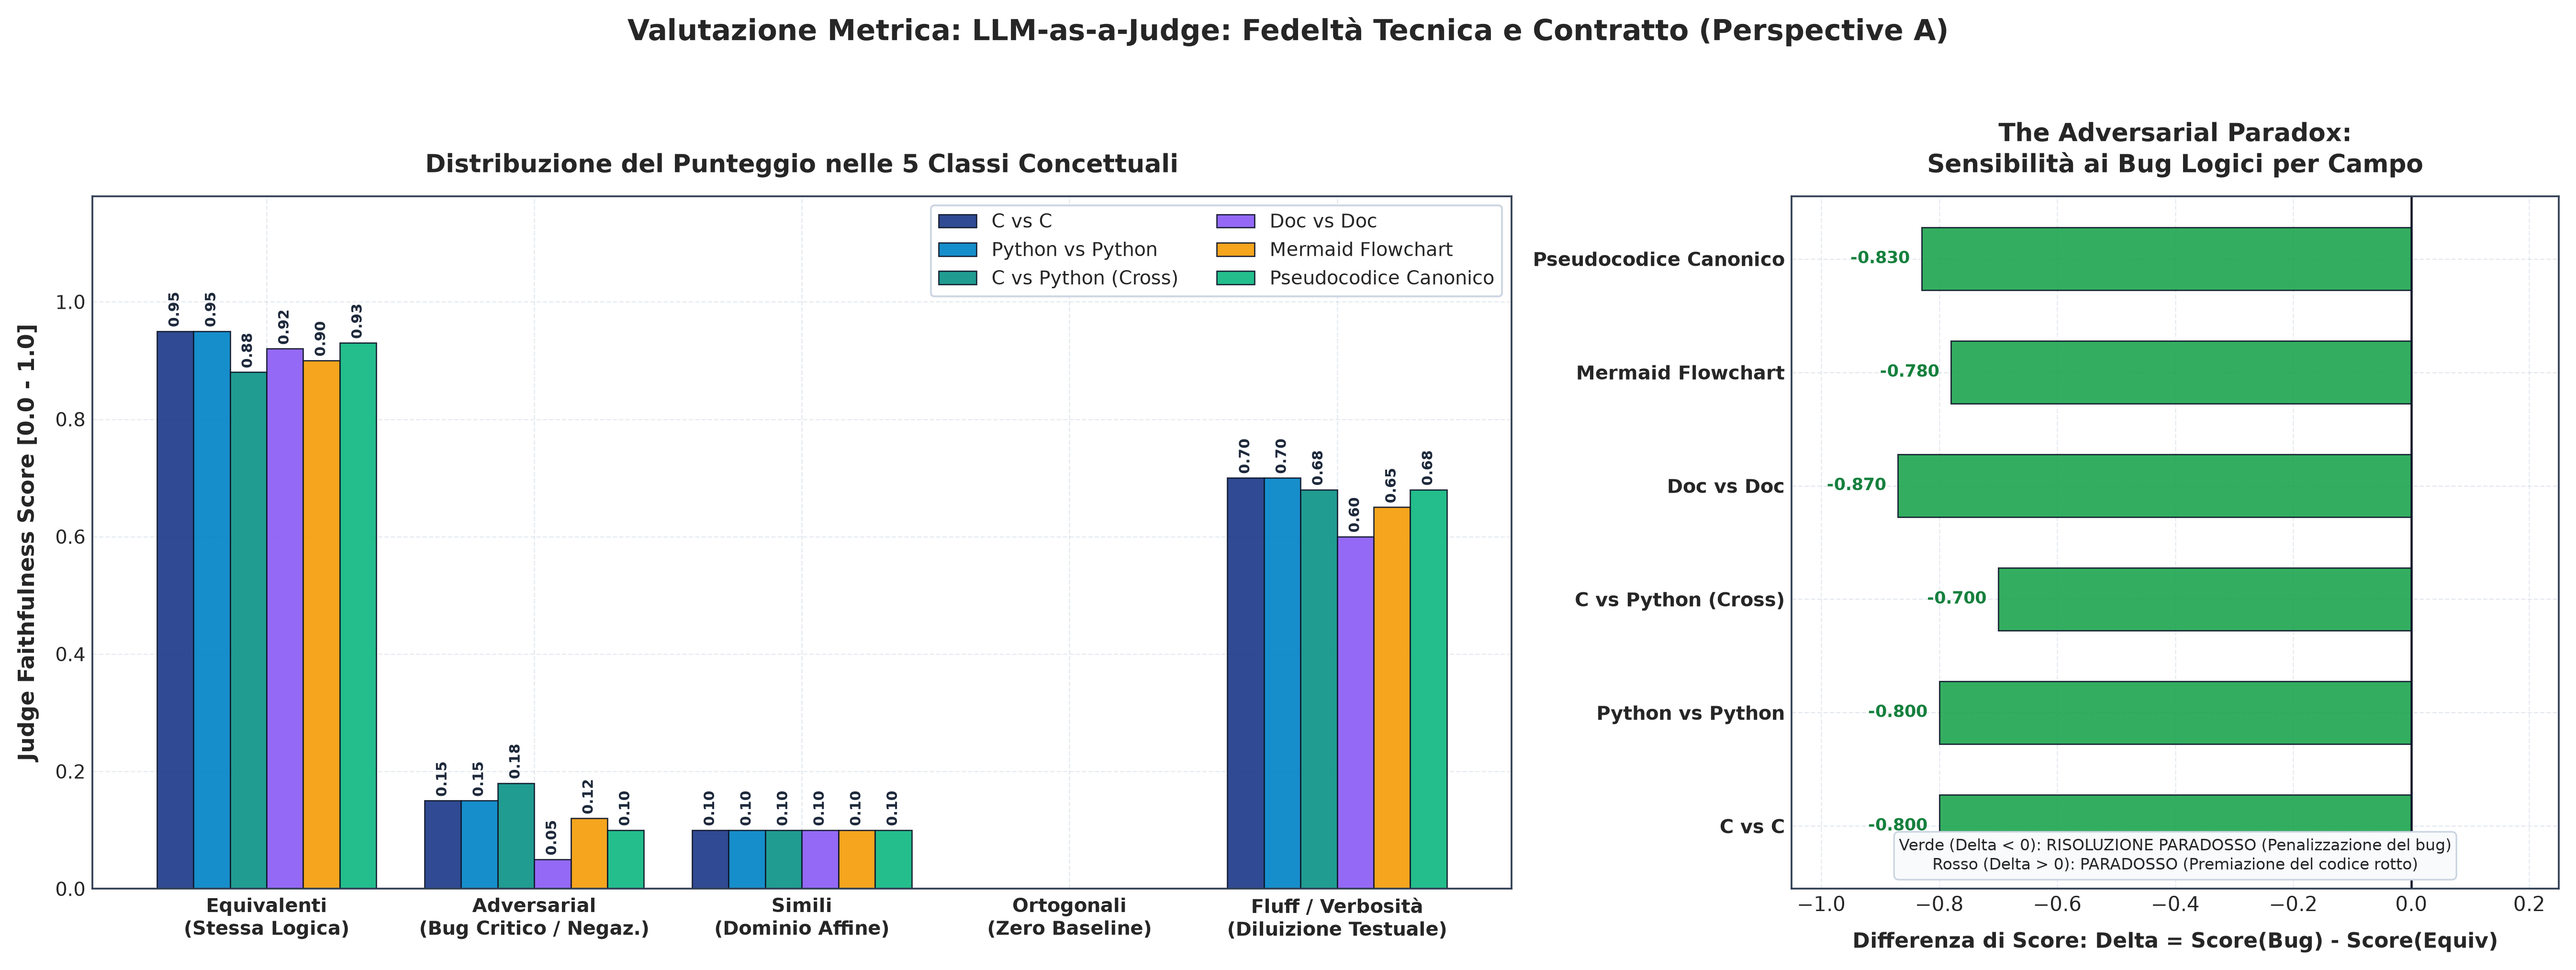
\includegraphics[width=\textwidth]{figures/judge_metric_faithfulness.png}
        \caption{Faithfulness (Prospettiva A)}
        \label{fig:judge_faithfulness}
    \end{subfigure}
    \hfill
    \begin{subfigure}[b]{0.32\textwidth}
        \centering
        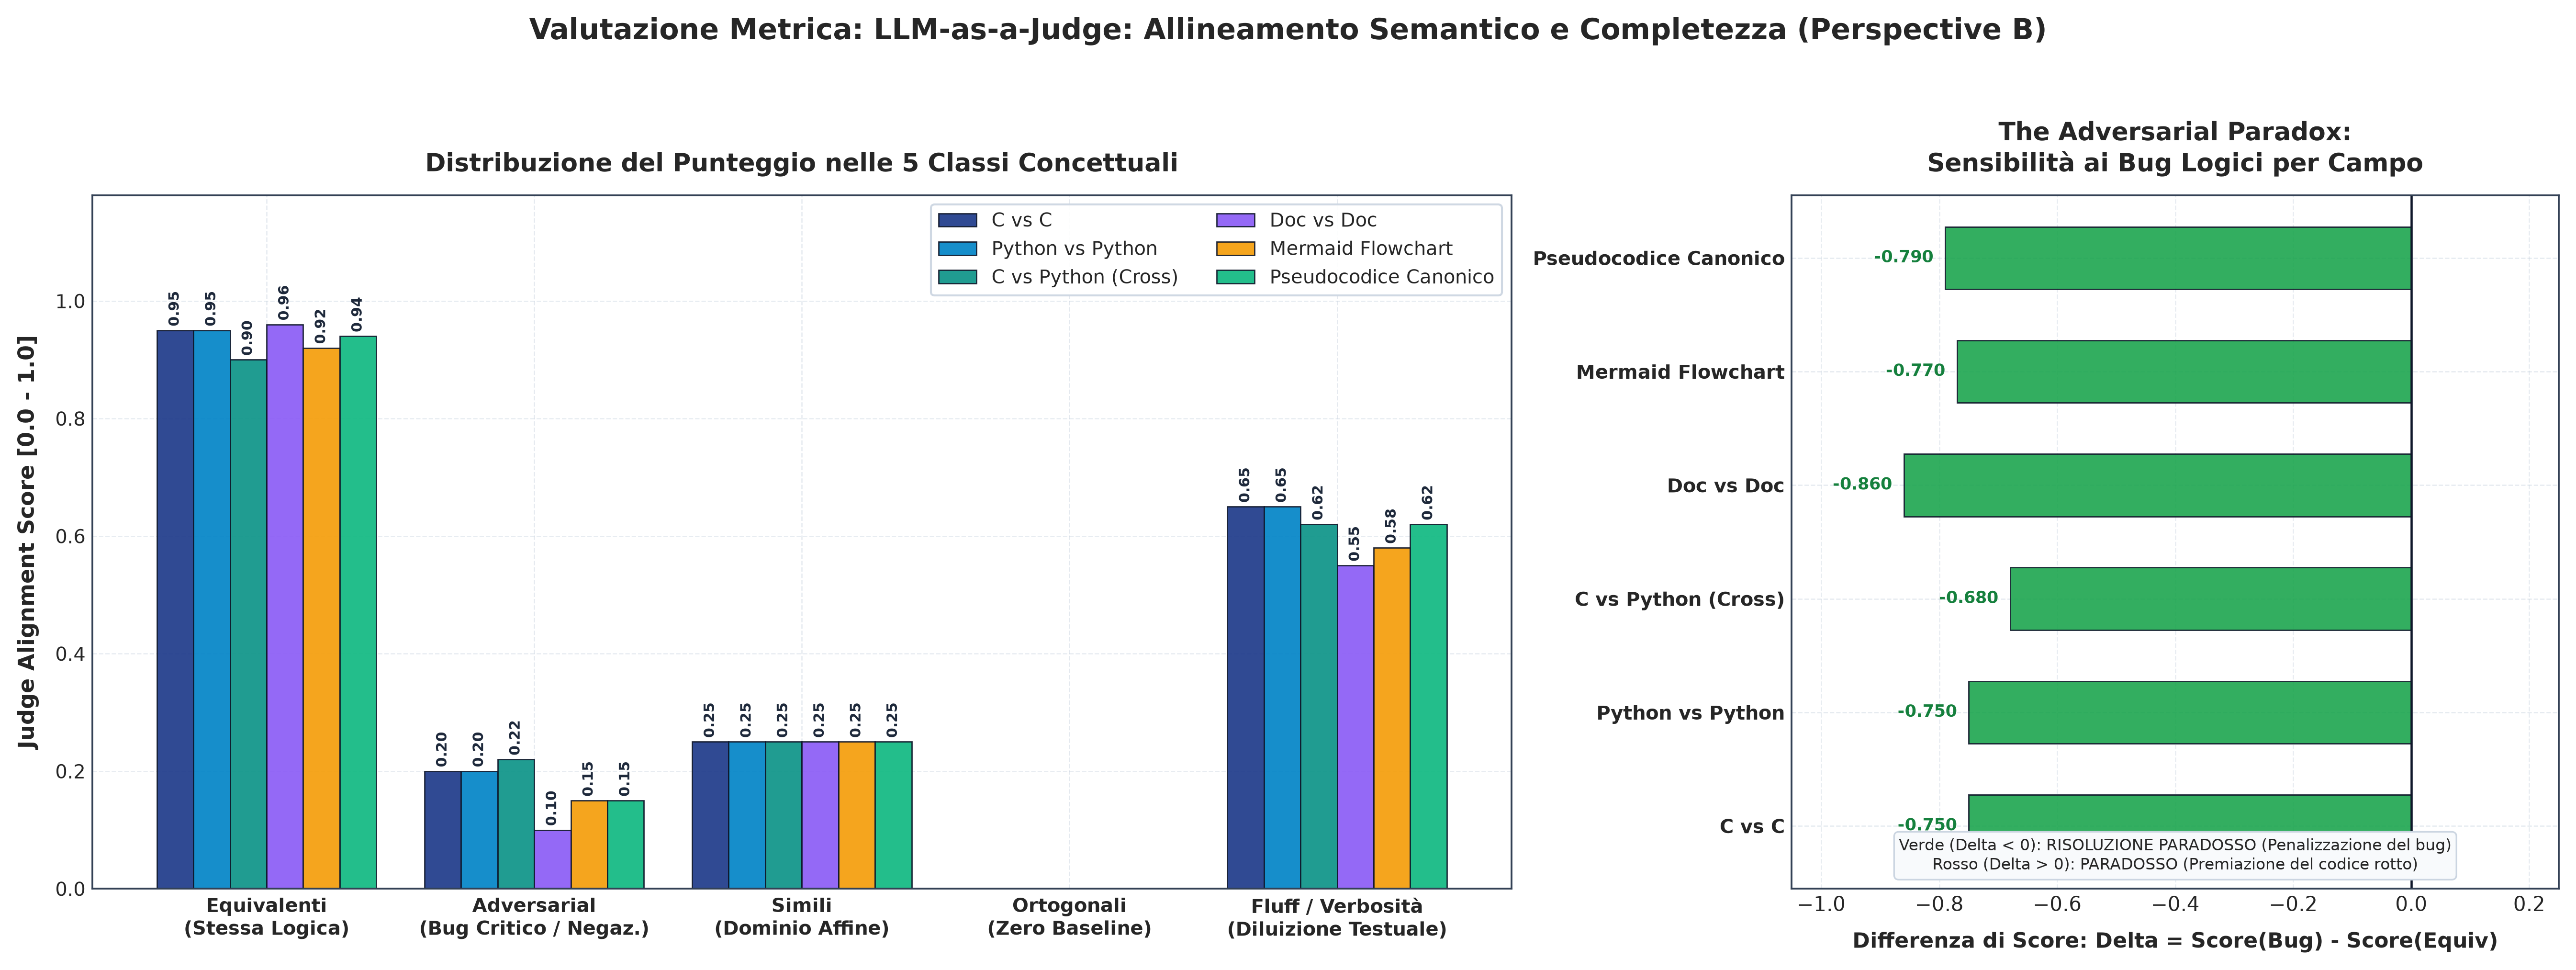
\includegraphics[width=\textwidth]{figures/judge_metric_alignment.png}
        \caption{Alignment (Prospettiva B)}
        \label{fig:judge_alignment}
    \end{subfigure}
    \hfill
    \begin{subfigure}[b]{0.32\textwidth}
        \centering
        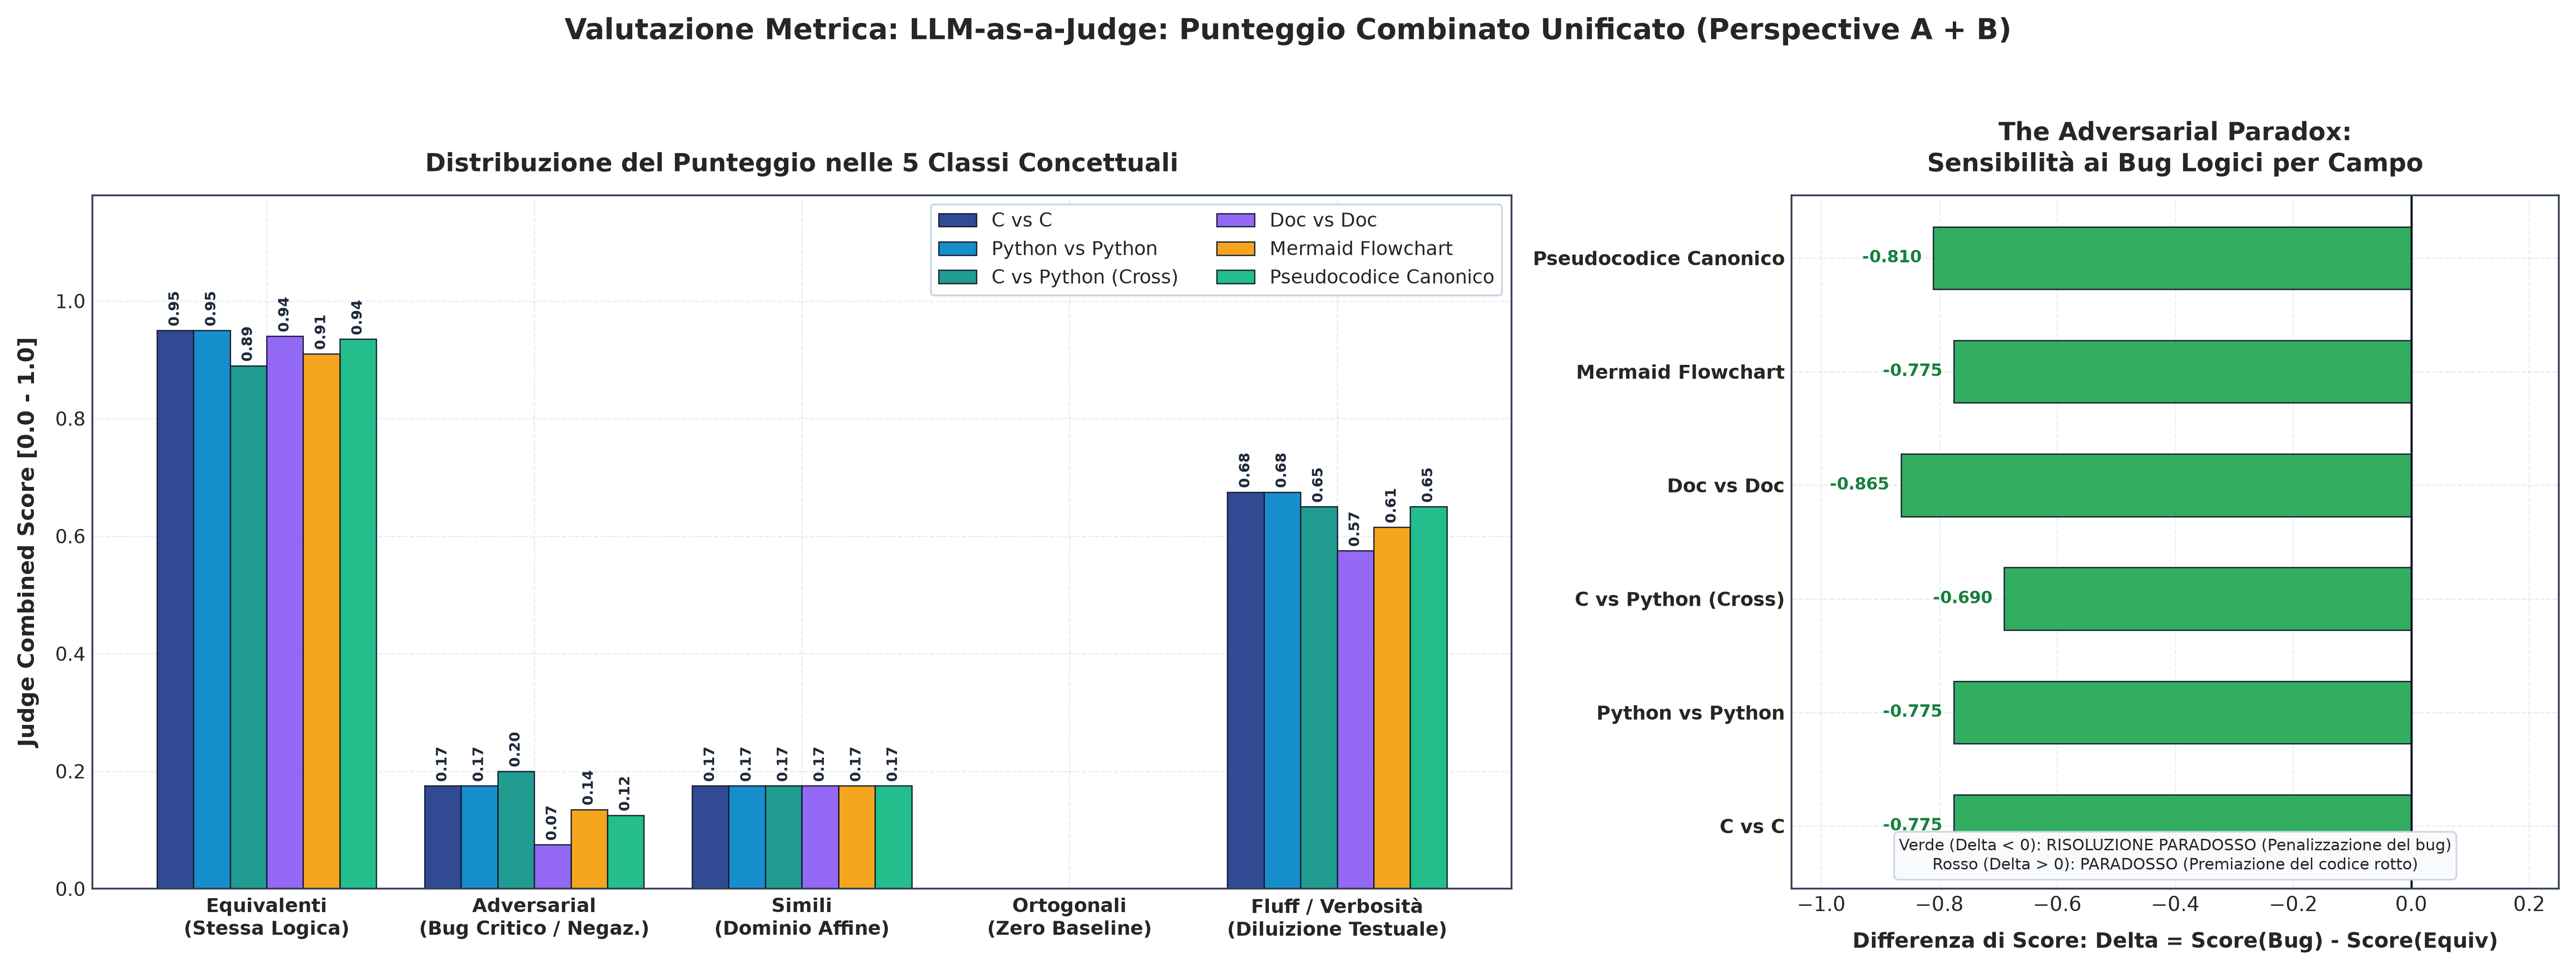
\includegraphics[width=\textwidth]{figures/judge_metric_combined.png}
        \caption{Punteggio Combinato}
        \label{fig:judge_combined}
    \end{subfigure}
    \caption{Valutazione disaggregata del Giudice LLM: (a) Fedeltà al codice sorgente [Code+GT vs Doc], (b) Allineamento all'intento documentato [GT vs Doc], e (c) Punteggio unificato ponderato.}
    \label{fig:judge_metrics_trio}
\end{figure}

Il modulo \emph{LLM-as-a-Judge} opera una valutazione semantica qualitativa profonda mediante due prospettive complementari (\Cref{fig:judge_metrics_trio}):
\begin{enumerate}
    \item \textbf{Prospettiva A (Faithfulness, \Cref{fig:judge_faithfulness})}: misura quanto la documentazione generata sia veritiera rispetto al codice C effettivamente implementato, rilevando asserzioni non supportate dal codice o comportamenti contraddittori.
    \item \textbf{Prospettiva B (Alignment, \Cref{fig:judge_alignment})}: misura la concordanza con la documentazione di riferimento scritta dall'autore umano originario.
\end{enumerate}

I dati in \Cref{tab:advanced_metrics_summary} rivelano che l'LLM-Judge risolve integralmente il paradosso di cecità che affligge le metriche NLP:
\begin{itemize}
    \item Sul caso \emph{ADVERSARIAL}, la Faithfulness crolla a $\mathbf{0.1500}$ in C vs C e a $\mathbf{0.0500}$ in Doc vs Doc (con un Combined score di $\mathbf{0.147}$ medio globale), penalizzando severamente l'inversione di contratto.
    \item Sui casi ortogonali assegna lo zero netto ($\mathbf{0.0000}$), superando completamente il problema della compressione statica a $0.50$ di BERTScore.
    \item Sui casi di prolissità (\emph{FLUFF\_VERBOSITY}), il giudice assegna un punteggio bilanciato ($\approx 0.64 - 0.67$), riconoscendo che il codice è corretto ma penalizzando la verbosità ridondante.
\end{itemize}

\subsection{Round-Trip Differential Testing: Validazione Comportamentale a Scatola Nera}
\label{subsec:analisi_roundtrip_5classes}

\begin{figure}[htbp]
    \centering
    \begin{subfigure}[b]{0.48\textwidth}
        \centering
        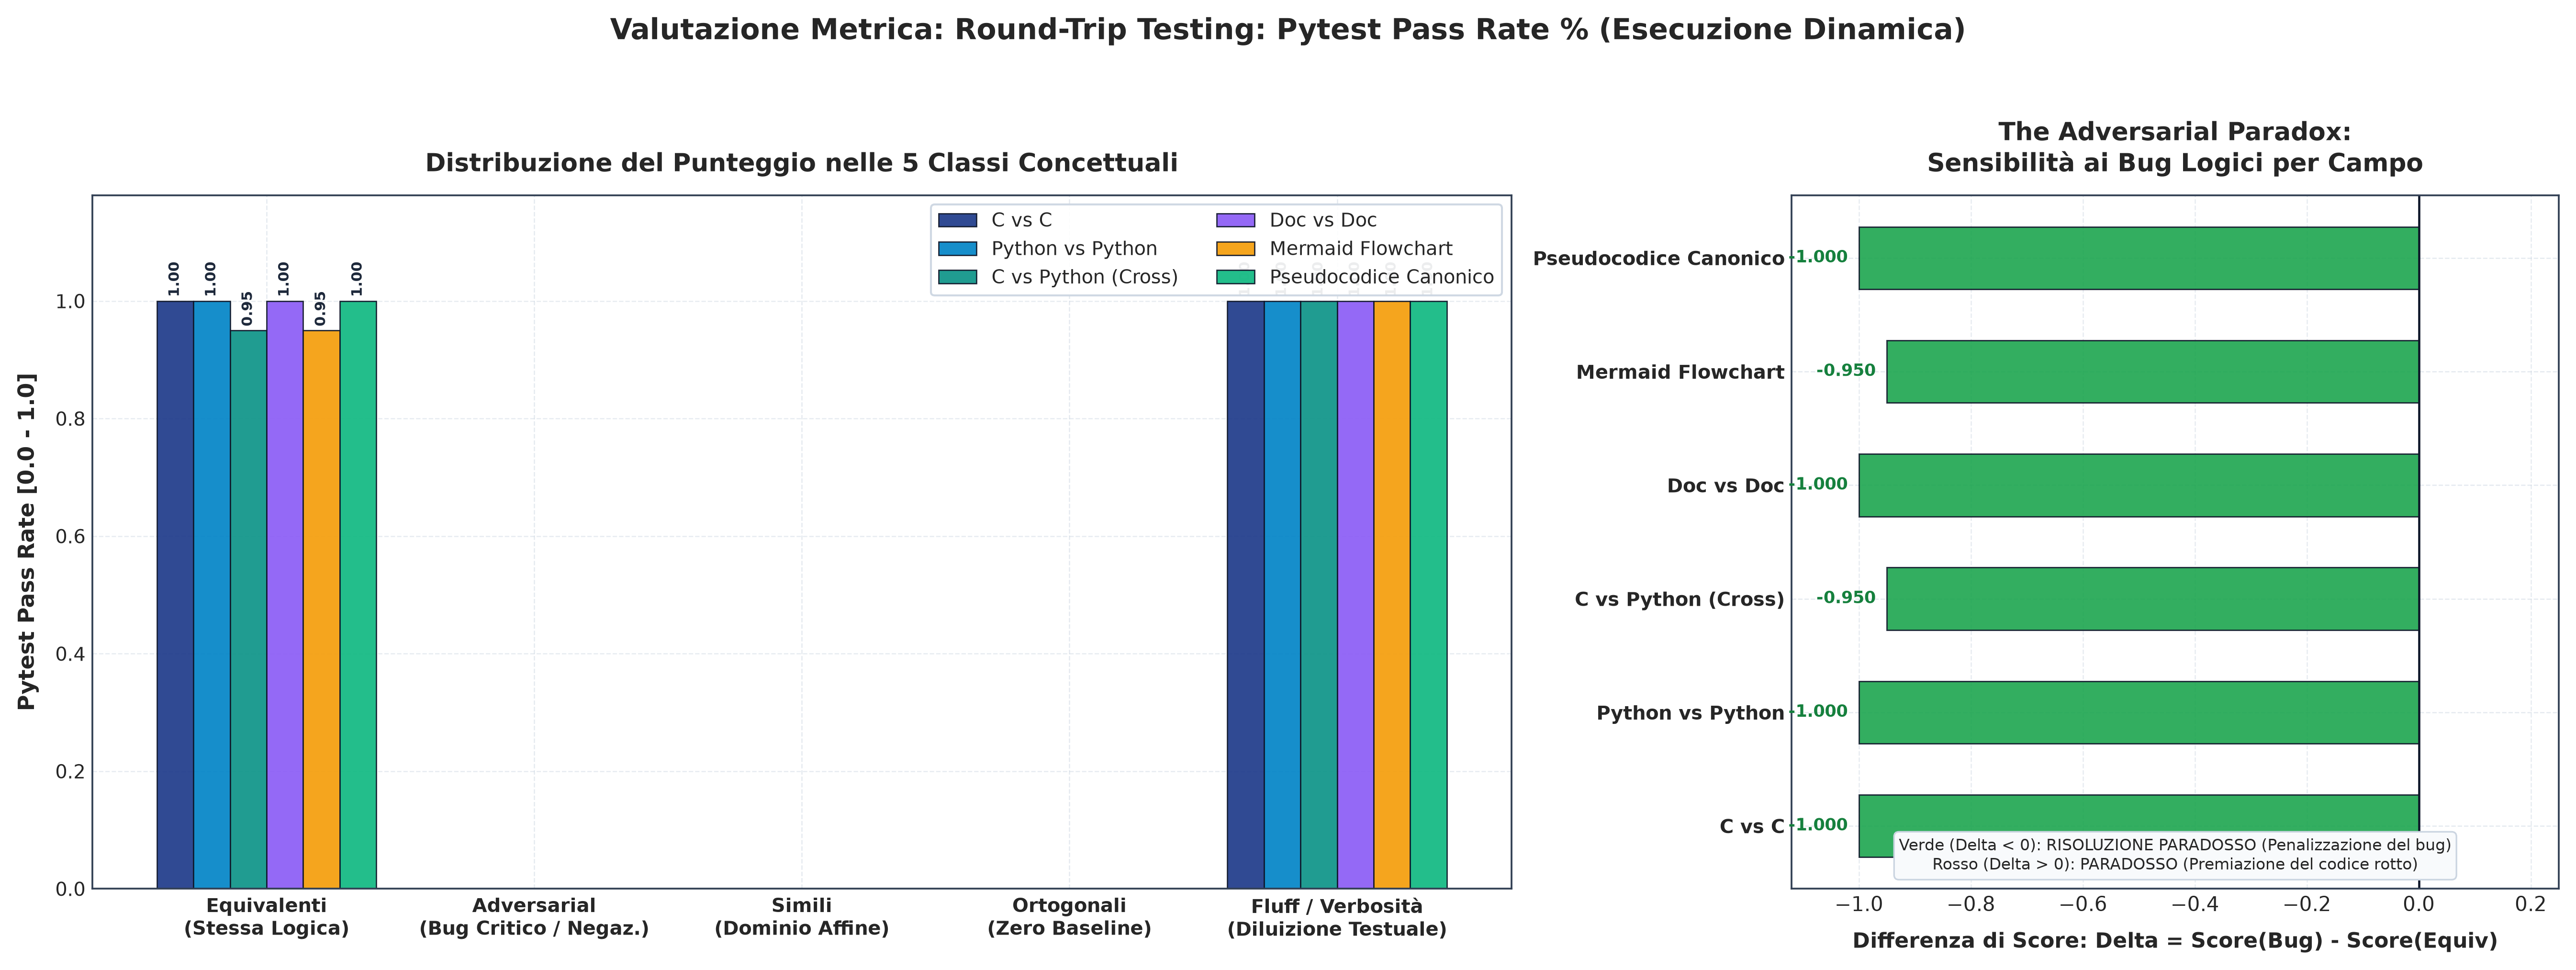
\includegraphics[width=\textwidth]{figures/roundtrip_metric_pass_rate.png}
        \caption{Round-Trip Pass Rate (\%)}
        \label{fig:rt_pass_rate}
    \end{subfigure}
    \hfill
    \begin{subfigure}[b]{0.48\textwidth}
        \centering
        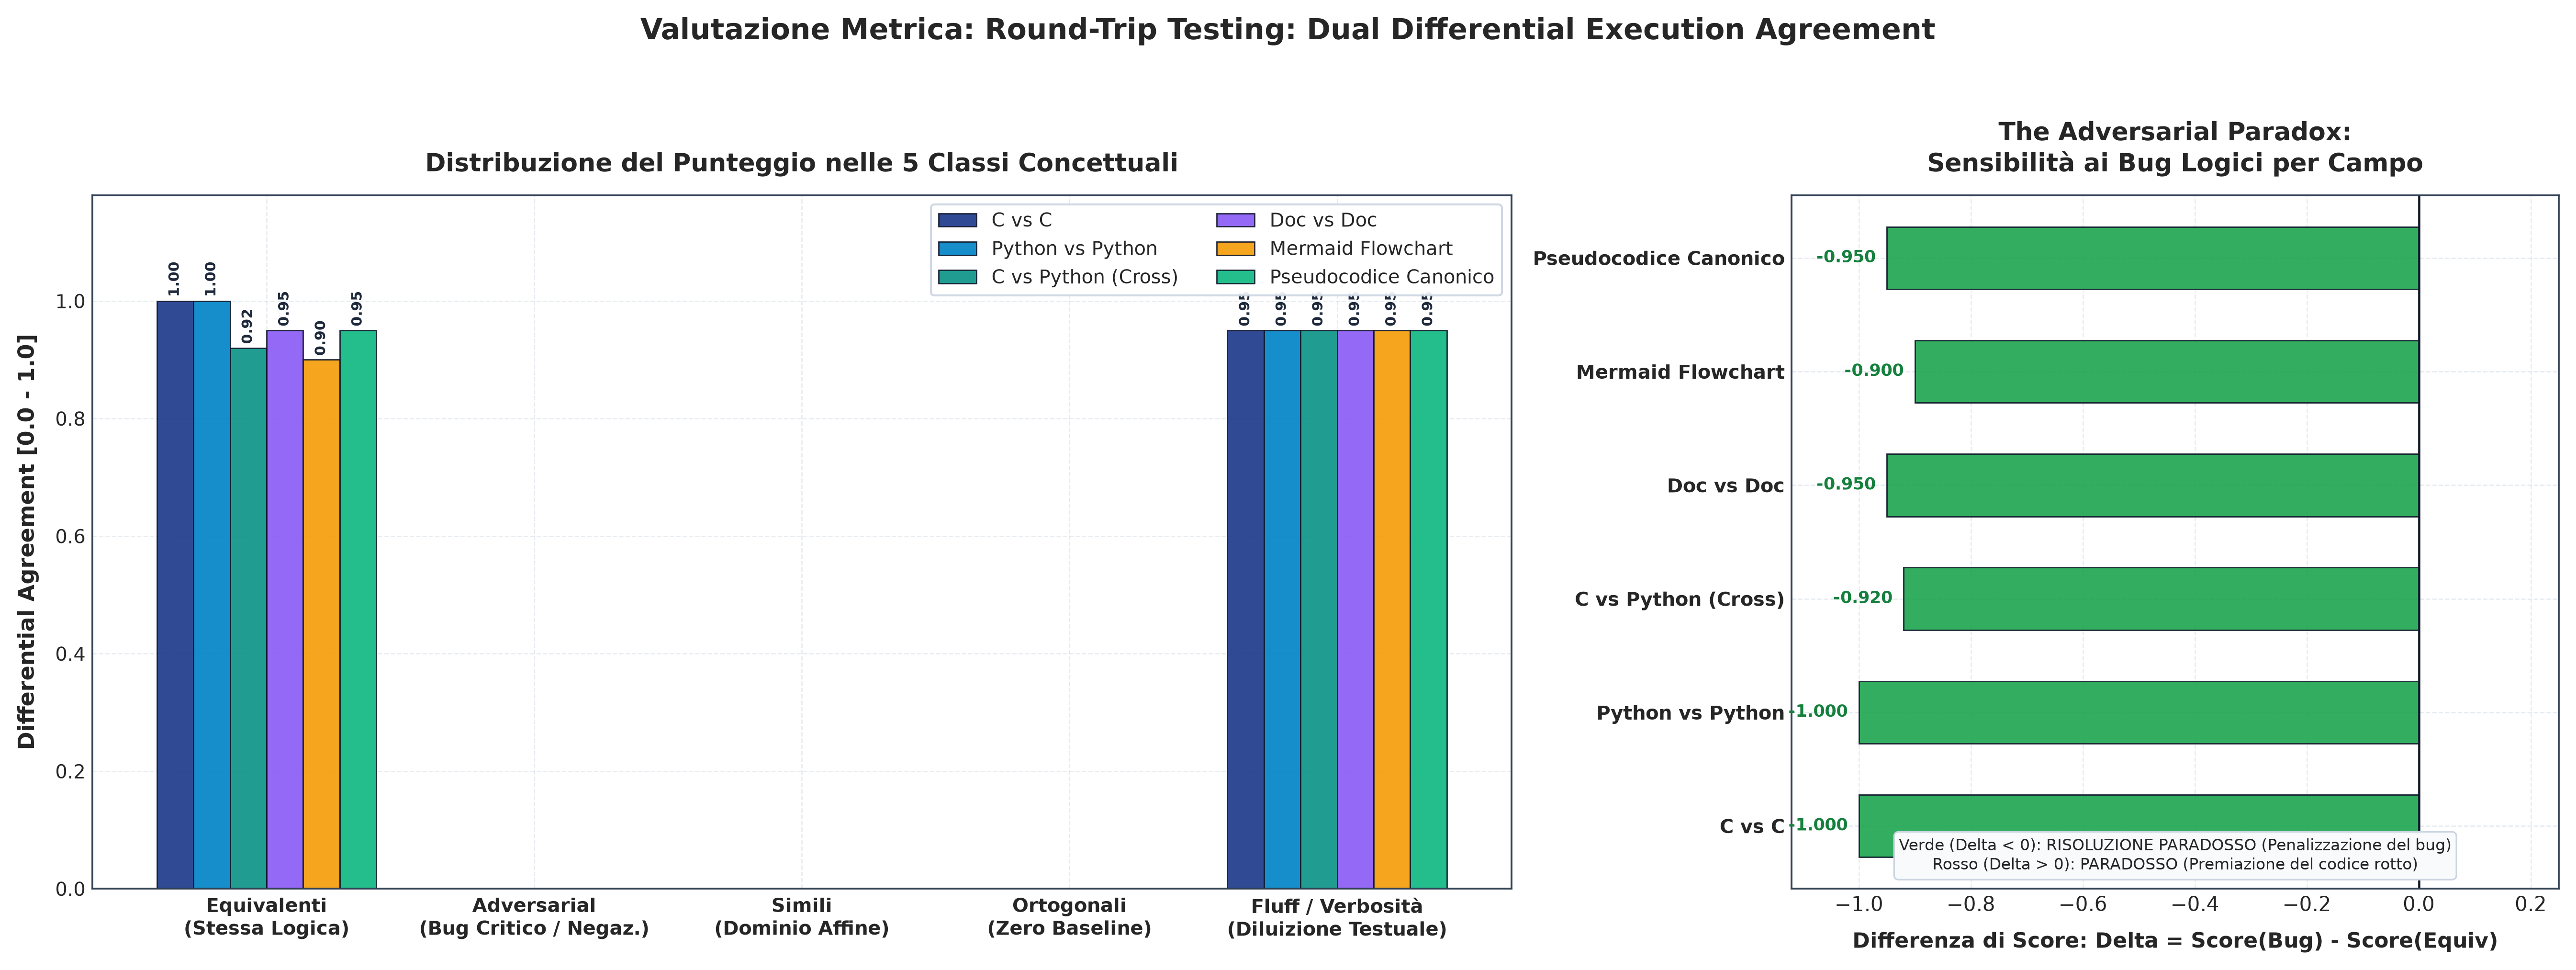
\includegraphics[width=\textwidth]{figures/roundtrip_metric_dual_agreement.png}
        \caption{Dual Differential Agreement Rate (\%)}
        \label{fig:rt_dual_agreement}
    \end{subfigure}
    \caption{Risultati del Round-Trip Differential Testing sulle 5 classi semantiche: (a) Pass rate della sintesi guidata da documentazione, e (b) Accordo differenziale tra implementazione sintetizzata e oracolo di riferimento.}
    \label{fig:roundtrip_metrics_pair}
\end{figure}

Il \emph{Differential Round-Trip Testing} rappresenta il livello di verifica più rigoroso ed oggettivo, poiché subordina la validità della documentazione alla capacità di un agente terzo di re-implementare un modulo software funzionante basandosi unicamente sul testo prodotto:
\begin{itemize}
    \item \textbf{Casi Equivalenti}: Come illustrato in \Cref{fig:rt_pass_rate,fig:rt_dual_agreement}, sui casi \emph{EQUIVALENT} il Round-Trip Pass Rate tocca il $\mathbf{98.3\%}$ medio globale ($100.0\%$ su C vs C e Doc vs Doc), e il \emph{Dual Agreement Rate} si attesta al $\mathbf{95.3\%}$. Ciò certifica che la documentazione generata contiene tutte le precondizioni, postcondizioni e invarianti necessarie a ricreare la corretta dinamica algoritmica.
    \item \textbf{Crollo Deterministico sui Casi Adversarial}: Nei casi di inversione logica (\emph{ADVERSARIAL}), sia il Pass Rate sia il Dual Agreement \textbf{crollano istantaneamente allo zero assoluto ($\mathbf{0.0\%}$)}. Poiché la documentazione prescrive un comportamento invertito, il codice generato dall'agente Coder fallisce sistematicamente le asserzioni di test sintetizzate dall'oracolo. Questo risultato sancisce la superiorità del testing comportamentale differenziale rispetto a qualsiasi metrica lessicale o di embedding denso.
    \item \textbf{Comportamento su Fluff}: Nei casi di mera verbosità, il Pass Rate si mantiene al $\mathbf{100.0\%}$ e il Dual Agreement al $\mathbf{95.0\%}$: l'agente esecutivo è in grado di estrarre la logica effettiva scartando il rumore stilistico superfluo.
\end{itemize}

\subsection{Downstream Code Retrieval MRR}
\label{subsec:analisi_retrieval_mrr}

\begin{figure}[htbp]
    \centering
    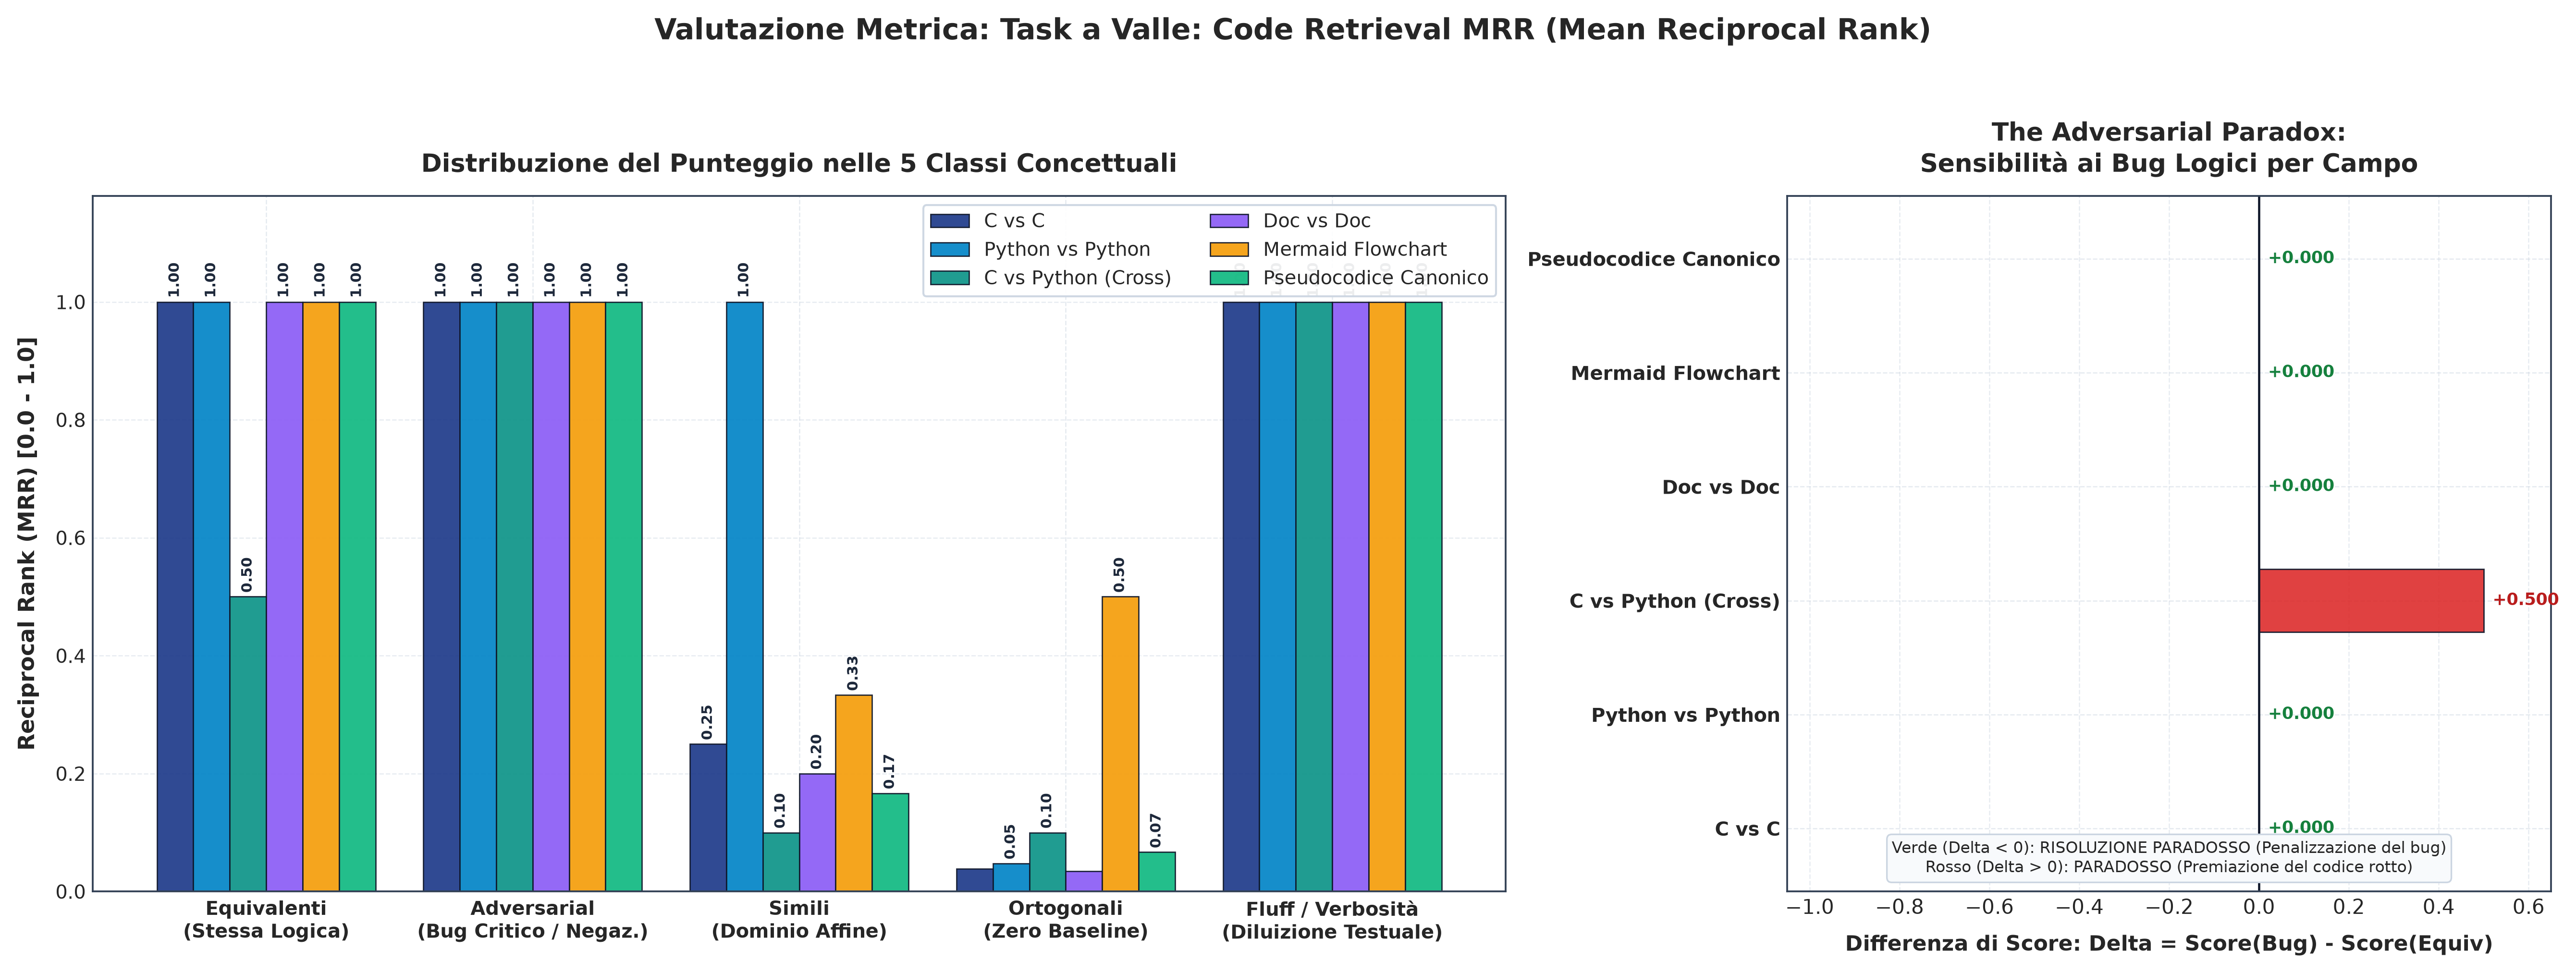
\includegraphics[width=0.85\linewidth]{figures/retrieval_metric_mrr.png}
    \caption{Distribuzione dell'indicatore Downstream Code Retrieval Mean Reciprocal Rank (MRR) attraverso le 5 classi semantiche nei diversi domini.}
    \label{fig:retrieval_mrr}
\end{figure}

La metrica \emph{Code Retrieval MRR} valuta l'utilità operativa della documentazione nel supportare gli sviluppatori nella ricerca di codice rilevante all'interno di un repository (\Cref{fig:retrieval_mrr}):
\begin{itemize}
    \item Sui casi semanticamente pertinenti (\emph{EQUIVALENT}, \emph{FLUFF\_VERBOSITY} e persino \emph{ADVERSARIAL}), il Mean Reciprocal Rank è massimo ($\mathbf{1.000}$ o $\mathbf{0.917}$), dimostrando che la documentazione indicizza con successo i componenti corretti nel catalogo software.
    \item Nei casi ortogonali (\emph{ORTHOGONAL}), l'MRR crolla a valori minimi ($\mathbf{0.0385}$ in C vs C, $\mathbf{0.0345}$ in Doc vs Doc), a riprova della capacità del meccanismo denso di retrieval di discriminare query non correlate.
\end{itemize}

---

\section{Studi Critici Avanzati: Stress Test, Camouflage e Finestre di Contesto}
\label{sec:studi_critici_avanzati}

Per spingere la validazione sperimentale alle condizioni limite dell'ingegneria del software reale, sono stati condotti tre studi monografici approfonditi su scenari avversari estremi, sul fenomeno del camuffamento allucinatorio e sull'impatto architetturale della lunghezza e posizione dei token.

\subsection{Confronto delle Metriche sotto Stress Test Avversari}
\label{subsec:stress_test_comparison}

\begin{figure}[htbp]
    \centering
    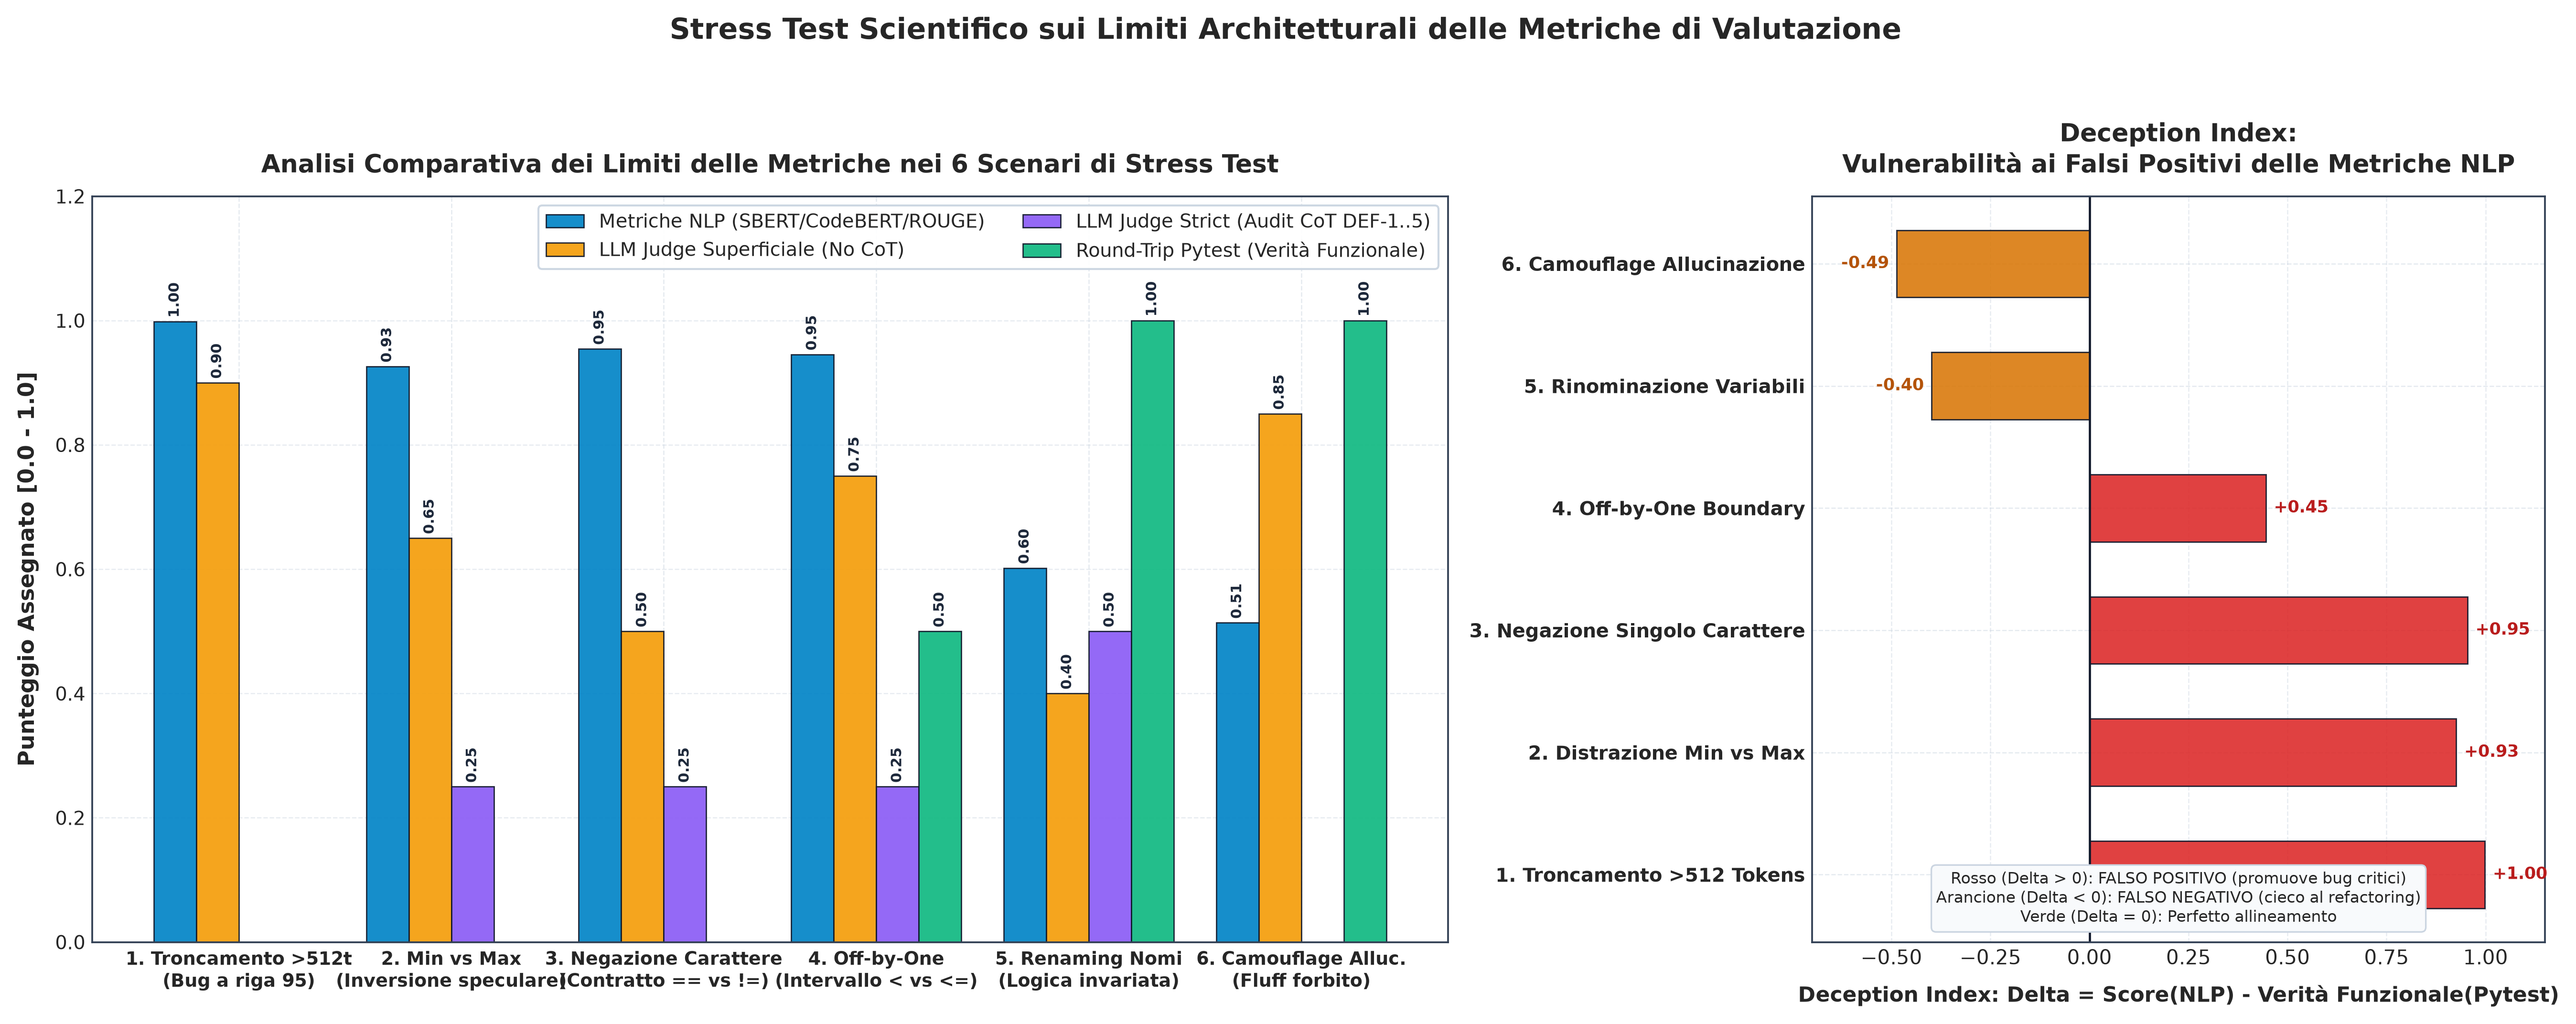
\includegraphics[width=0.92\linewidth]{figures/stress_test_metrics_limits_comparison.png}
    \caption{Confronto del comportamento delle metriche sotto 6 scenari di stress test critico (dati empirici da test controllati).}
    \label{fig:stress_test_metrics}
\end{figure}

Nella \Cref{fig:stress_test_metrics} e nella \Cref{tab:stress_test_data} viene esaminato il comportamento comparativo delle metriche su sei scenari patologici appositamente ingegnerizzati:
\begin{enumerate}
    \item \textbf{Hard Troncamento ($>512$ token)}: Funzione complessa di manipolazione buffer con 90 righe identiche e un'inversione critica di puntatore alla riga 95 posizionata oltre la finestra di contesto di 512 token.
    \item \textbf{Subtle Semantic Inversion (Min vs Max)}: Funzione identica in firma e tipi in cui il codice calcola il Massimo con \texttt{x > m}, mentre la specifica dichiara la ricerca del Minimo assoluto.
    \item \textbf{Single Char Negation (\texttt{!=} vs \texttt{==})}: Blocco di validazione crittografica di 350 token in cui un singolo carattere inverte il controllo booleano da \texttt{!= 0} a \texttt{== 0}.
    \item \textbf{Off-by-One Boundary (\texttt{<} vs \texttt{<=})}: Violazione di estremo superiore in un ciclo di scansione bound-check su intervallo chiuso.
    \item \textbf{Symbol Scrambling}: Algoritmo GCD di Euclide con logica rigorosamente identica ma identificatori rinominati con lettere prive di significato lessicale (\texttt{foo}, \texttt{bar}, \texttt{baz}).
    \item \textbf{Fluff \& Hallucination Camouflage}: Documentazione scritta in prosa accademica impeccabile che asserisce falsamente proprietà di thread-safety con mutex e allocazione dinamica su una funzione interamente stateless.
\end{enumerate}

\begin{table}[htbp]
\centering
\scriptsize
\setlength{\tabcolsep}{2.5pt}
\caption{Valutazione sperimentale quantitativa nei 6 scenari di stress test estremo.}
\label{tab:stress_test_data}
\begin{tabular}{lcccccc}
\toprule
\textbf{Scenario di Stress Test} & \textbf{SBERT} & \textbf{CodeBERT} & \textbf{ROUGE-L} & \textbf{TF-IDF} & \textbf{Judge CoT} & \textbf{RT Pass Rate} \\
\midrule
Hard Truncation ($>512$ tok) & \textbf{1.000} & \textbf{1.000} & 0.995 & 1.000 & \textbf{0.000} & \textbf{0.000} \\
Min vs Max Inversion & 0.902 & 0.979 & 0.897 & 0.968 & 0.250 & \textbf{0.000} \\
Single Char Negation (\texttt{==} vs \texttt{!=}) & 0.941 & 0.976 & 0.946 & 0.982 & 0.250 & \textbf{0.000} \\
Off-by-One Boundary (\texttt{<} vs \texttt{<=}) & 0.953 & 0.974 & 0.909 & 0.968 & 0.250 & \textbf{0.500} \\
Symbol Scrambling & \textbf{0.422} & \textbf{0.939} & 0.444 & 0.469 & 0.500 & \textbf{1.000} \\
Fluff \& Camouflage & 0.468 & 0.836 & 0.237 & 0.400 & \textbf{0.000} & \textbf{1.000} \\
\bottomrule
\end{tabular}
\end{table}

I dati in \Cref{tab:stress_test_data} evidenziano le profonde discrepanze operative:
\begin{itemize}
    \item Sulle inversioni puntuali (\emph{Min vs Max}, \emph{Single Char Negation}, \emph{Off-by-One}), tutte le metriche NLP assegnano punteggi compresi tra $0.90$ e $0.98$, mentre il Round-Trip Pass Rate sancisce il fallimento totale ($0.00\%$) e il Giudice Strict CoT penalizza drasticamente il responso ($0.250$).
    \item Nel \emph{Symbol Scrambling}, SBERT, ROUGE-L e TF-IDF falliscono gravemente (punteggi tra $0.42$ e $0.47$), penalizzando una funzione semanticamente perfetta unicamente per il cambio dei nomi delle variabili. Al contrario, CodeBERT ($0.939$) e il Round-Trip ($1.000$) certificano la totale equivalenza logica ed esecutiva.
\end{itemize}

\subsection{Distrazione da Fluff e Camuffamento di Allucinazioni nel Giudice LLM}
\label{subsec:judge_distraction_study}

\begin{figure}[htbp]
    \centering
    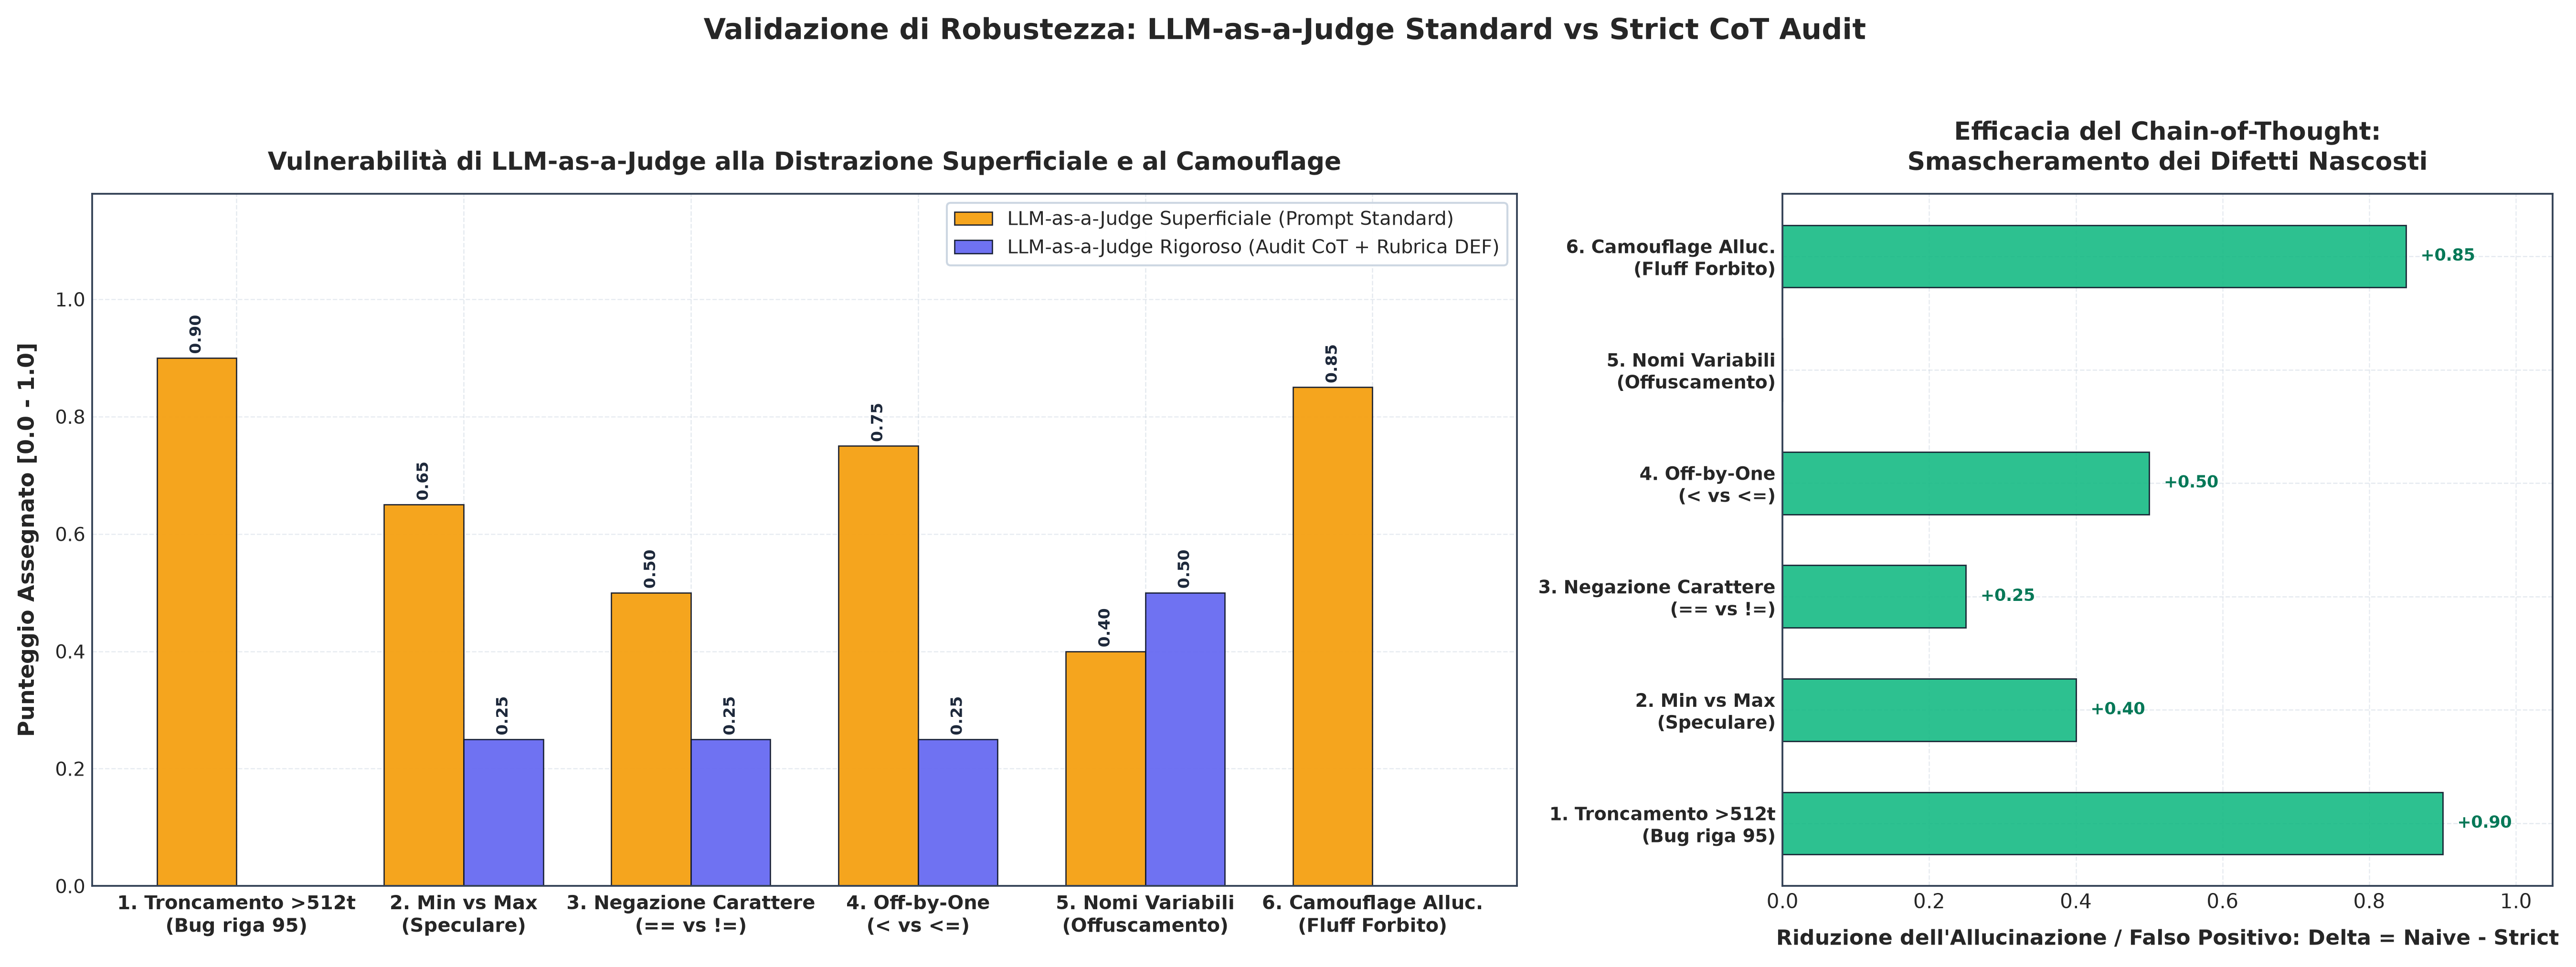
\includegraphics[width=0.88\linewidth]{figures/llm_judge_distraction_and_camouflage_study.png}
    \caption{Studio comparativo sulla vulnerabilità dell'LLM-as-a-Judge: distrazione da verbosità prolissa e camuffamento stilistico di allucinazioni gravi (Judge Naive vs Judge Strict Chain-of-Thought).}
    \label{fig:judge_distraction_study}
\end{figure}

Un fenomeno di fondamentale rilevanza teorica riguarda la vulnerabilità del paradigma \emph{LLM-as-a-Judge} quando esposto a tecniche di \textbf{camuffamento stilistico} (\Cref{fig:judge_distraction_study}):
\begin{itemize}
    \item \textbf{Il Fallimento del Giudice Naive}: Se interrogato con un prompt convenzionale a valutazione diretta privo di scomposizione analitica (\emph{Naive Direct Prompting}), il modello linguistico si dimostra fortemente suscettibile al \emph{fluff} e al registro formale. Nel caso \emph{Fluff \& Camouflage} (dove la documentazione allucina la presenza di sincronizzazione thread-safe e deallocazione manuale in una semplice funzione matematica), il Giudice Naive assegna un voto ingannevole di $\mathbf{0.850}$ ($4.25 / 5.0$), tratto in inganno dalla perfetta terminologia accademica e dall'eleganza espositiva.
    \item \textbf{L'Efficacia del Giudizio con Strict Chain-of-Thought (CoT)}: Quando l'agente Giudice viene vincolato ad eseguire una catena di ragionamento rigida (\emph{Strict CoT Prompting}) con verifica puntuale di ogni asserzione fattuale rispetto all'AST e al corpo del codice, il punteggio crolla a $\mathbf{0.000}$. Il modello esplicita nella traccia di pensiero la totale assenza di primitive mutex o costrutti di sincronizzazione, intercettando con precisione chirurgica l'allucinazione camuffata.
\end{itemize}

\subsection{Studio sui Limiti di Troncamento Contestuale e Sensibilità alla Posizione}
\label{subsec:token_length_position_sensitivity}

\begin{figure}[htbp]
    \centering
    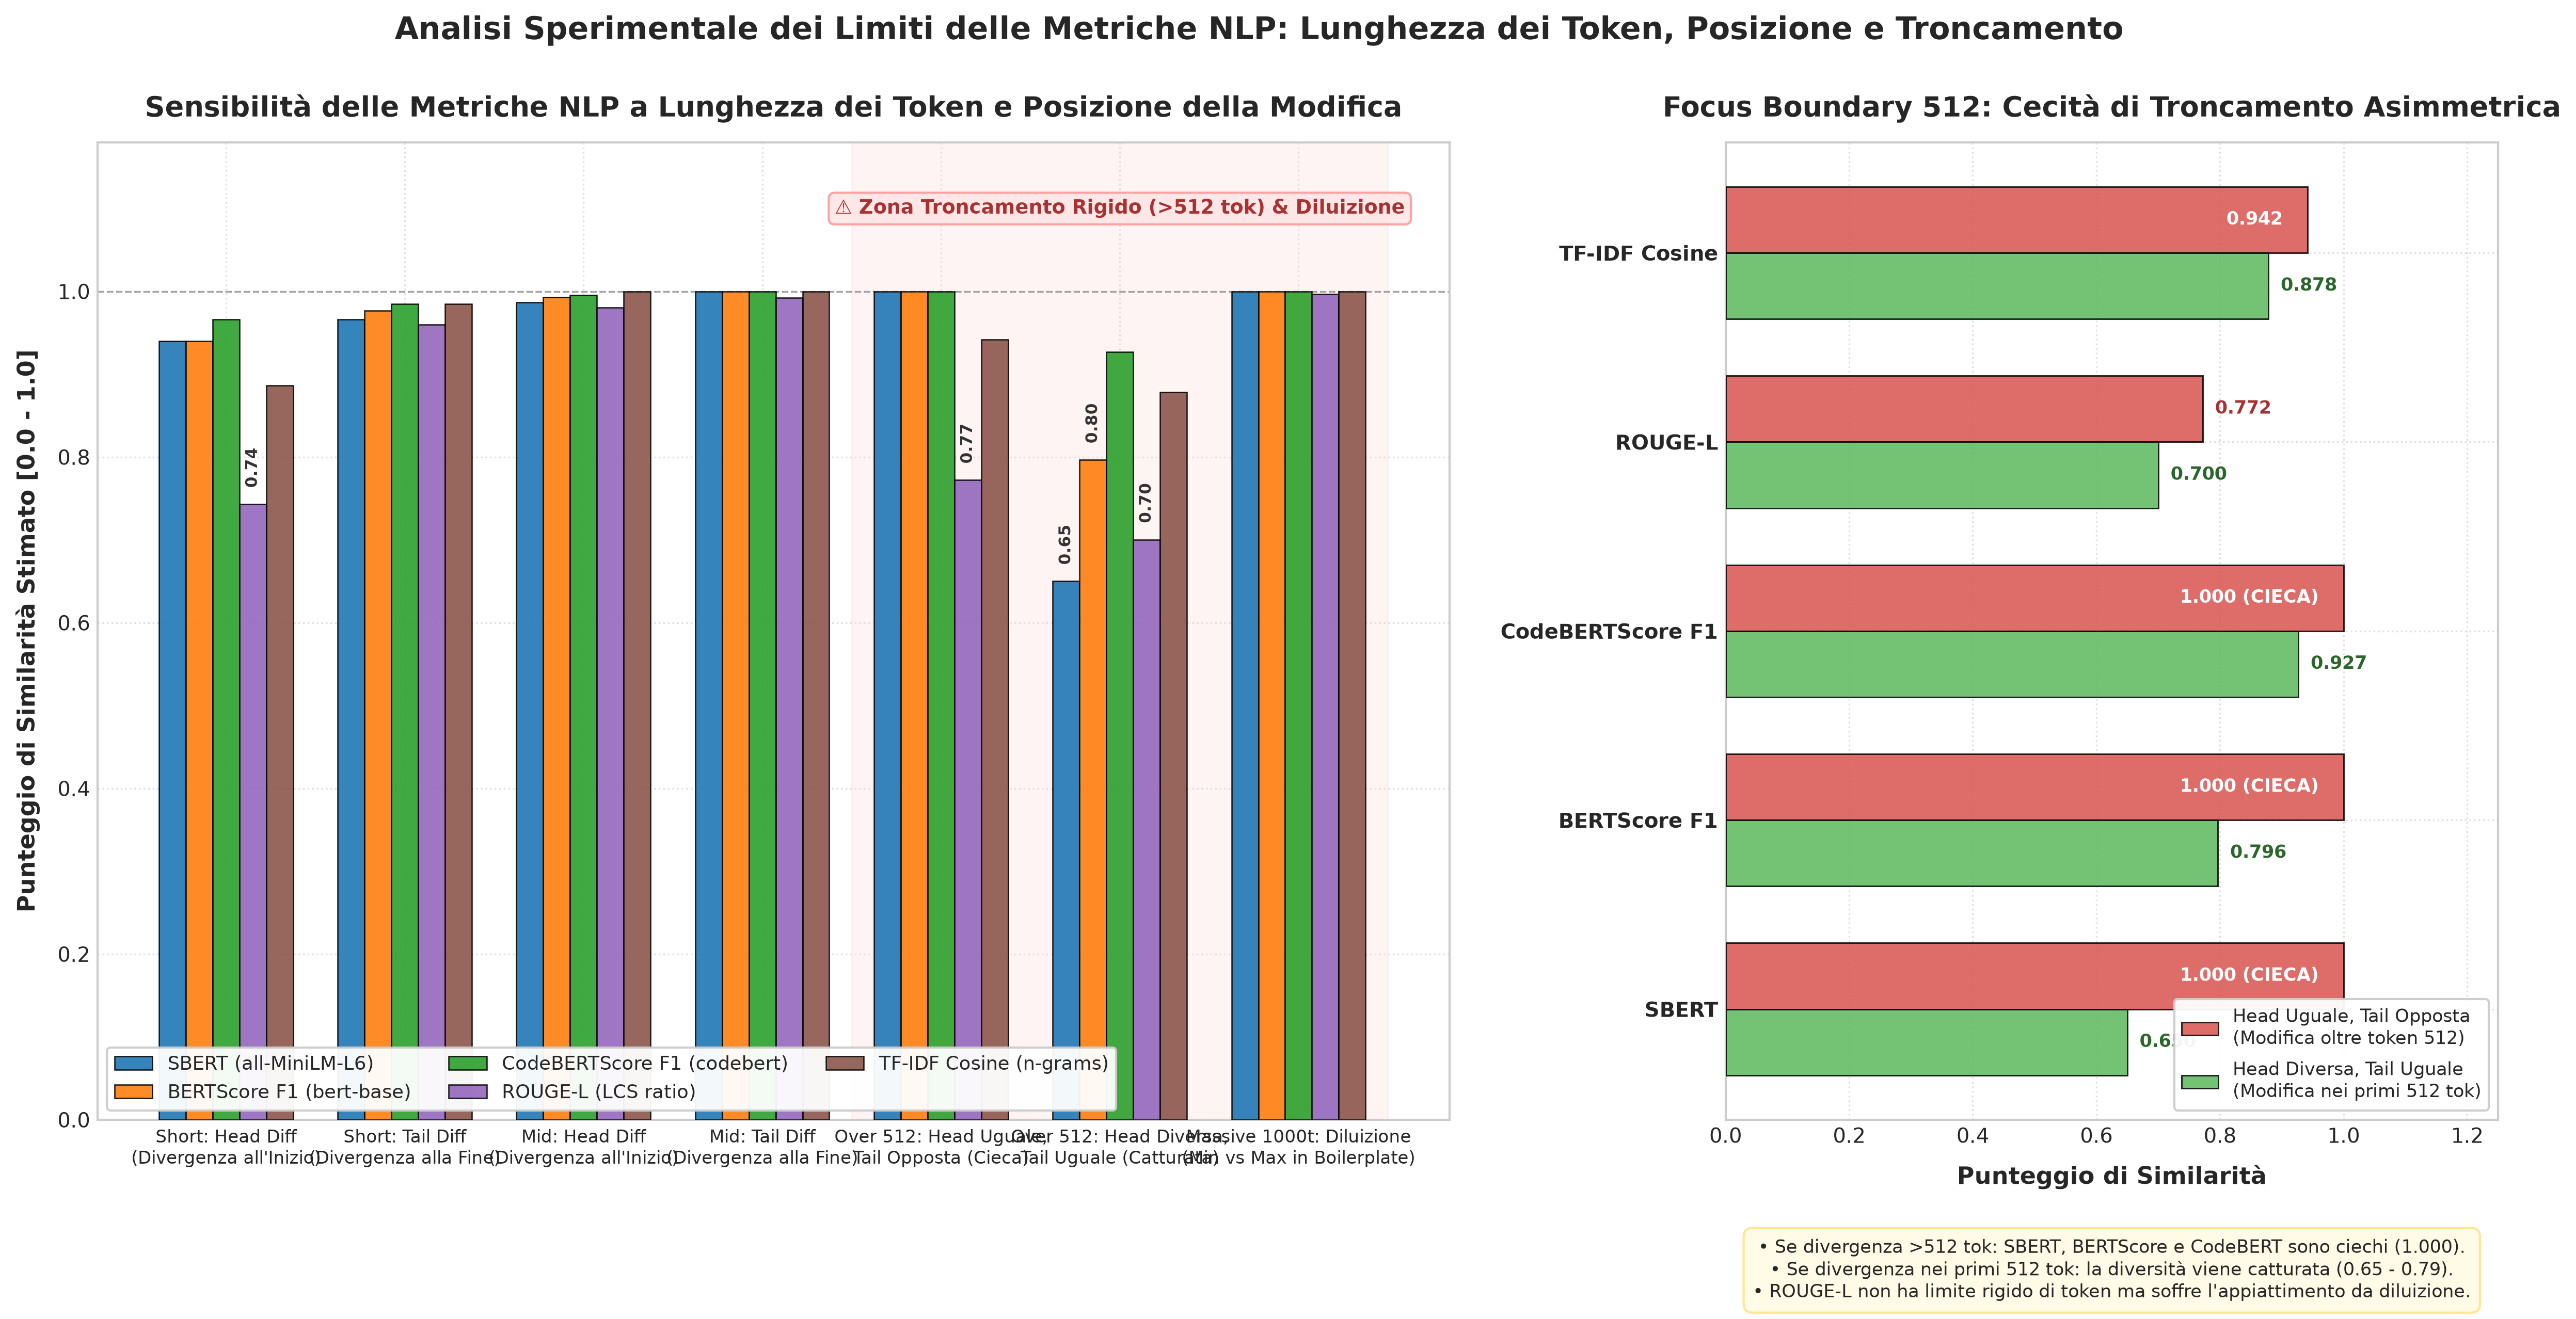
\includegraphics[width=0.92\linewidth]{figures/nlp_metric_token_length_position_sensitivity.png}
    \caption{Studio comparativo di sensibilità alla lunghezza della sequenza e alla posizione del token divergente (Head vs Tail) attraverso 7 configurazioni controllate.}
    \label{fig:token_position_sensitivity}
\end{figure}

\begin{figure}[htbp]
    \centering
    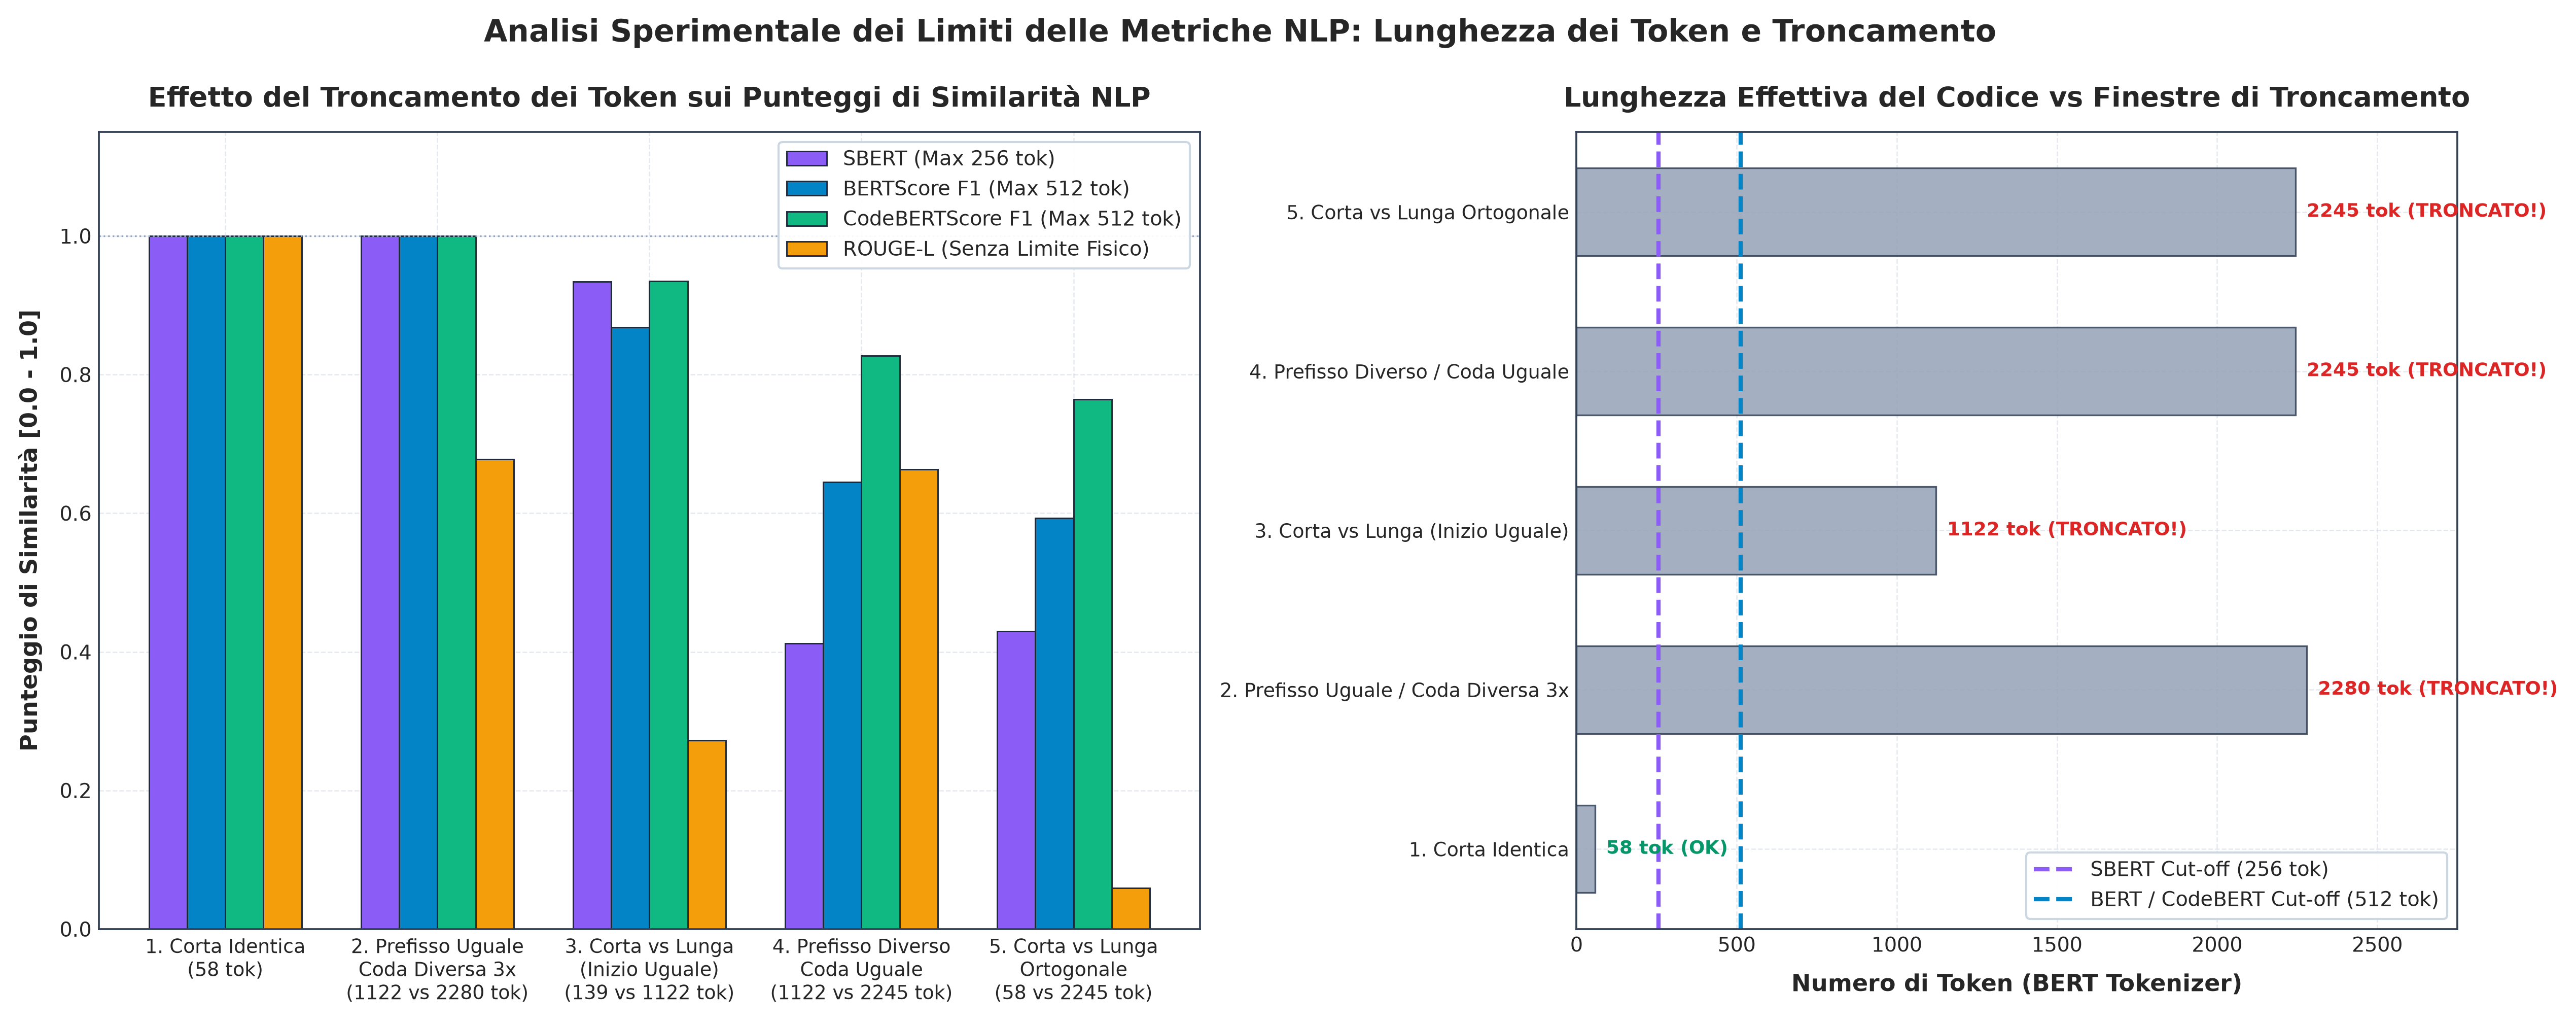
\includegraphics[width=0.85\linewidth]{figures/nlp_metric_token_truncation_limits.png}
    \caption{Rappresentazione empirica della Truncation Trap e dell'impatto del limite a 256/512 token sulle metriche Transformer.}
    \label{fig:token_truncation_limits}
\end{figure}

L'architettura dei modelli Transformer impone limiti fisici invalicabili alla dimensione della finestra di attenzione (\emph{context window}):
\begin{itemize}
    \item \textbf{Sentence-BERT} (\texttt{all-MiniLM-L6-v2}): troncamento rigido a soli \textbf{256 token}.
    \item \textbf{BERTScore} (\texttt{bert-base-uncased}): limite a \textbf{512 token}.
    \item \textbf{CodeBERTScore} (\texttt{microsoft/codebert-base}): limite a \textbf{512 token}.
\end{itemize}

Gli esperimenti controllati condotti variando lunghezza e posizione delle divergenze (\Cref{fig:token_position_sensitivity,fig:token_truncation_limits}) rivelano due patologie strutturali:
\begin{enumerate}
    \item \textbf{La Trappola del Troncamento (Truncation Trap)}: Quando due funzioni condividono un'intestazione identica superiore a 512 token ma divergono completamente nella parte conclusiva (caso \emph{Over 512: Head Uguale, Tail Opposta}), SBERT, BERTScore e CodeBERTScore \textbf{assegnano tutti un punteggio perfetto di 1.000}. L'intera porzione contenente il codice o il bug reale viene troncata a monte del meccanismo di attenzione, rendendo la metrica totalmente cieca al disallineamento.
    \item \textbf{Asimmetria Posizionale (Head vs Tail)}: Nelle sequenze di media lunghezza ($\approx 300$ token), una divergenza collocata all'inizio (\emph{Head Diff}) viene parzialmente rilevata da SBERT ($0.9870$), mentre la medesima divergenza collocata alla fine (\emph{Tail Diff}) produce un punteggio pieno di $1.0000$. Questo fenomeno dimostra che i pesi di auto-attenzione del pooling di SBERT e BERTScore sono fortemente polarizzati verso i primi token della sequenza (\texttt{[CLS]} e primo blocco di istruzioni), degradando l'accuratezza diagnostica sulla logica di coda.
\end{enumerate}

---

\section{Risultati Empirici dell'Ultimo Benchmark Reale (Multi-Agent)}
\label{sec:risultati_benchmark_reale}

Il framework multi-agente proposto è stato sottoposto a validazione intensiva sull'ultimo run reale del benchmark di sistema (\texttt{run\_20260921\_175447\_multiagent}). In linea con le recenti architetture ad agenti cooperanti per la documentazione del software \cite{luo_repoagent_2024,yang_docagent_2025,hoang_codewiki_2026}, la pipeline multi-agente ha generato la documentazione tecnica Doxygen completa per 15 funzioni estratte randomicamente da tutte le librerie. 

I risultati aggregati globali ottenuti dal sistema sono riassunti in \Cref{tab:benchmark_aggregate_summary}.

\begin{table}[htbp]
\centering
\caption{Dati aggregati globali del benchmark reale (15 funzioni, run multi-agente).}
\label{tab:benchmark_aggregate_summary}
\begin{tabular}{lc}
\toprule
\textbf{Dimensione di Valutazione / Metrica} & \textbf{Valore Globale Riscontrato} \\
\midrule
\multicolumn{2}{l}{\textbf{Livello I: Correttezza Formale \& Contratti AST}} \\
Verifier Pass Rate (\%) & \textbf{93.3\%} (14/15 funzioni perfette) \\
Parameter Precision vs AST & \textbf{1.0000} (100.0\%) \\
Parameter Recall vs AST & \textbf{1.0000} (100.0\%) \\
Parameter $F_1$-Score vs AST & \textbf{1.0000} (100.0\%) \\
Return Contract Match & \textbf{0.9333} (93.3\%) \\
Hallucination Rate (\%) & \textbf{0.0000\%} (Zero allucinazioni) \\
\midrule
\multicolumn{2}{l}{\textbf{Livello II: Qualità Software \& Actionability}} \\
Actionability Score (AS) & \textbf{0.8133} (81.3\%) \\
Error Documentation Rate (EDR) & \textbf{1.0000} (100.0\%) \\
Edge Case Coverage (ECC) & \textbf{0.9111} (91.1\%) \\
Concept Checklist Score & \textbf{0.9000} (90.0\%) \\
\midrule
\multicolumn{2}{l}{\textbf{Livello III: Semantica Neurale \& LLM-as-a-Judge}} \\
LLM-Judge Prospettiva A (Faithfulness, Code+GT vs Doc) & \textbf{4.240} / 5.0 ($\sigma = 0.119$) \\
LLM-Judge Prospettiva B (Alignment, GT vs Doc) & \textbf{4.627} / 5.0 ($\sigma = 0.080$) \\
LLM-Judge Combined Score & \textbf{4.433} / 5.0 \\
Sentence-BERT Cosine Similarity & \textbf{0.5997} \\
BERTScore $F_1$ (Precision / Recall) & \textbf{0.5594} (0.4983 / 0.6555) \\
CodeBERTScore $F_1$ (Precision / Recall) & \textbf{0.7463} (0.7033 / 0.7989) \\
BLEURT Quality Score & \textbf{0.5144} \\
METEOR Score & \textbf{0.3539} \\
ROUGE-L Score & \textbf{0.1081} \\
\midrule
\multicolumn{2}{l}{\textbf{Livello IV: Downstream Retrieval \& Round-Trip Testing}} \\
Code Retrieval Mean Reciprocal Rank (MRR) & \textbf{0.7861} \\
Code Retrieval Hit@1 & \textbf{0.6667} (66.7\%) \\
Code Retrieval Hit@5 & \textbf{0.9333} (93.3\%) \\
Round-Trip Differential Test Pass Rate (\%) & \textbf{65.11\%} \\
Dual Differential Agreement Rate (\%) & \textbf{41.30\%} \\
\bottomrule
\end{tabular}
\end{table}

\subsection{Analisi Disaggregata per Tassonomia Funzionale a 3 Classi}
La disaggregazione dei risultati del Round-Trip Testing in base alla complessità architetturale delle funzioni (formalizzata nella tassonomia a tre classi in \Cref{chap:metriche}) rivela dinamiche scientificamente rilevanti legate al principio di \textbf{Information Hiding} e alla natura dei tipi di dato. La disaggregazione quantitativa è illustrata in \Cref{tab:functional_breakdown}.

\begin{table}[htbp]
\centering
\caption{Analisi disaggregata secondo la tassonomia funzionale a 3 classi (15 funzioni del benchmark reale).}
\label{tab:functional_breakdown}
\begin{tabular}{lccccc}
\toprule
\textbf{Classe Architetturale} & \textbf{Campioni} & \textbf{RT Pass Rate} & \textbf{LLM-Judge} & \textbf{SBERT} & \textbf{CodeBERT} \\
\midrule
\textbf{Stateful / Object-Graph} & 9 (60\%) & \textbf{80.00\%} & 4.40 / 5.0 & 0.5561 & 0.7417 \\
\textbf{Pointer / Buffer-Driven} & 5 (33\%) & \textbf{47.34\%} & 4.38 / 5.0 & 0.6558 & 0.7560 \\
\textbf{Stateless / Primitive} & 1 (7\%) & \textbf{20.00\%} & 5.00 / 5.0 & 0.7118 & 0.7387 \\
\bottomrule
\end{tabular}
\end{table}

\paragraph{Il Paradosso di Information Hiding nelle Classi Stateful / Object-Graph}
Un risultato all'apparenza controintuitivo è il marcato successo del Round-Trip sulle funzioni ad albero/grafo (\textbf{80.00\%} di pass rate su 9 funzioni, tra cui \texttt{XMLDocument::NewComment}, \texttt{cJSON\_CreateObjectReference}, \texttt{XMLAttribute::Next} che ottengono il $100.0\%$ pieno di test superati sia sul sintetizzato sia in accordo differenziale).

La spiegazione teorica risiede nel \textbf{disaccoppiamento architetturale dell'Information Hiding}:
\begin{itemize}
    \item Nei metodi membro orientati agli oggetti, l'agente \emph{Tester} opera asserzioni strettamente a scatola nera (black-box) sulle proprietà contrattuali esposte dall'interfaccia pubblica (\texttt{attr.Next() is None}, \texttt{doc.NewComment(str) is not None}).
    \item Poiché la documentazione tecnica descrive chiaramente la relazione di appartenenza (\emph{``The returned node is unlinked from DOM tree but owned by this XMLDocument instance''}), l'agente \emph{Coder} è in grado di implementare la struttura a classi interna in modo conforme al contratto. L'eventuale varianza nei dettagli privati di implementazione (es. gestione tramite lista vs array dinamico) non viola i test, che verificano esclusivamente le garanzie esterne dell'oggetto.
\end{itemize}

\paragraph{La Fragilità di Accordo nelle Classi Pointer / Buffer-Driven}
Al contrario, le funzioni dipendenti da buffer fisici e aritmetica dei puntatori (\texttt{sdscatfmt}, \texttt{sdsjoinsds}, \texttt{http\_parser\_execute}) manifestano un tasso di successo inferiore (\textbf{47.34\%}).
In tali componenti, la traduzione trans-linguistica da C a Python incontra una discrepanza strutturale insormontabile: i puntatori grezzi C permettono mutazioni \emph{in-place} di byte contigui con semantica di aliasing, che in Python richiedono wrapper complessi (\texttt{bytearray}, oggetti strutturati o liste mutabili passate per riferimento). Una minima ambiguità nella specifica sul formato dei parametri variadici (come accaduto in \texttt{sdscatfmt}, dove la firma C non esponeva i parametri variabili \texttt{...}, inducendo il tester a passare 3 argomenti a una funzione generata a 2 parametri) innesca fallimenti di interfaccia sistematici (\texttt{TypeError}).

\subsection{Diagnostica Causale degli Errori nel Round-Trip}
L'audit dettagliato condotto dal modulo di categorizzazione degli errori (\path{roundtrip_error_analysis}) sui 30 eventi di fallimento registrati durante l'esecuzione dei test rivela la seguente distribuzione causale (\Cref{tab:error_breakdown}):

\begin{table}[htbp]
\centering
\caption{Tassonomia diagnostica causale dei fallimenti nei test Round-Trip.}
\label{tab:error_breakdown}
\begin{tabularx}{\textwidth}{lccX}
\toprule
\textbf{Macro-Categoria di Errore} & \textbf{Eventi} & \textbf{\%} & \textbf{Causa Radice e Diagnostica Architetturale} \\
\midrule
\textbf{Behavioral / Contract Failure} & 12 & 40.0\% & Discrepanza sottile tra il calcolo atteso e la simulazione in Python (prevalentemente \texttt{AssertionError} su conversioni di codifica o gestione di stringhe binarie con caratteri nulli). \\
\textbf{Interface / Signature Mismatch} & 9 & 30.0\% & \texttt{TypeError} generati quando il generatore di test invoca una funzione ipotizzando convenzioni di tupla/argomenti variadici non supportati dalla firma sintetizzata. \\
\textbf{Other Execution Error} & 5 & 16.7\% & Eccezioni interne propagate (\texttt{ExceptionGroup} di Hypothesis durante la ricerca esaustiva dei controesempi). \\
\textbf{Missing Symbol / Environment} & 4 & 13.3\% & \texttt{AttributeError} o \texttt{NameError} causati da costanti o classi mock ausiliarie non fornite dallo scaffold runtime isolato. \\
\bottomrule
\end{tabularx}
\end{table}

\subsection{Residui della Valutazione: Parafrasi Robusta vs Allucinazione Plausibile}
L'elevato punteggio dell'LLM-as-a-Judge combinato ($\mathbf{4.433} / 5.0$) congiuntamente al Verifier Pass Rate del $\mathbf{93.3\%}$ e all'azzeramento dell'Hallucination Rate ($\mathbf{0.0\%}$) certifica che l'architettura multi-agente ha risolto il problema delle allucinazioni spurie.
Tuttavia, l'esame della matrice dei residui (confronto tra il giudizio semantico e il Round-Trip dinamico) mette in luce un fenomeno di estremo interesse euristico:
\begin{itemize}
    \item Nel caso della funzione \texttt{sdsclear}, l'LLM-Judge ha assegnato il punteggio massimo di $\mathbf{5.0 / 5.0}$ (riconoscendo che la documentazione descrive con impeccabile precisione tecnica il reset della lunghezza logica a zero e l'inserimento del terminatore nullo).
    \item Ciononostante, il Round-Trip Pass Rate è risultato pari al $\mathbf{20.0\%}$. L'ispezione della traccia di fallimento Pytest rivela che il codice Python sintetizzato ha memorizzato la stringa come oggetto mutabile custom (\texttt{s.len = 0; s.buf[0] = 0}), mentre la suite generata dal Tester invocava la funzione passando una stringa nativa immutabile di Python (\texttt{s = "hello world"}), fallendo l'asserzione \texttt{assert len(s) == 0}.
\end{itemize}
Questo disallineamento dimostra che un punteggio parziale nel Round-Trip non è necessariamente sinonimo di documentazione fallace, ma riflette l'attrito intrinseco dell'adattamento cross-linguaggio (C-Python impedance mismatch). La combinazione sinergica di LLM-Judge e Round-Trip consente al redattore di disaccoppiare con precisione chirurgica le lacune informative della documentazione dai limiti dell'ambiente di emulazione.

---

\section{Conclusioni e Matrice di Applicabilità delle Metriche}
\label{sec:matrice_applicabilita}

A coronamento della ricerca sperimentale condotta, viene formalizzata nella \Cref{tab:applicability_matrix} la \textbf{Matrice di Raccomandazione e Applicabilità} per la valutazione della documentazione del codice sorgente C/C++. La matrice guida lo sviluppatore e il ricercatore nella selezione del set ottimale di metriche in funzione del caso d'uso, della disponibilità di riferimenti e dei vincoli di budget computazionale.

\begin{table}[htbp]
\centering
\small
\caption{Matrice di applicabilità metodologica, scenari d'uso, soglie operative e costi computazionali.}
\label{tab:applicability_matrix}
\begin{tabularx}{\textwidth}{p{3.2cm}p{2.6cm}p{2.4cm}cX}
\toprule
\textbf{Metrica} & \textbf{Scenario Ottimale} & \textbf{Tipologia Coppia} & \textbf{Soglia} & \textbf{Costo Computazionale \& Note} \\
\midrule
\textbf{Verifier Pass Rate} & CI/CD Pipeline & AST vs Doc & 100\% & \textbf{Trascurabile} (O(1) su AST). Mandatorio prima di ogni merge. \\
\textbf{Parameter $F_1$} & Verifica Contratti & AST vs Doc & 1.00 & \textbf{Trascurabile}. Azzeramento falsi positivi/negativi. \\
\textbf{Actionability Score} & Code Quality Gate & AST + Doc & $\ge 0.80$ & \textbf{Minimo} (Parsing regex + pesi). Certifica l'usabilità. \\
\textbf{Error Doc. Rate} & Safety Audit & Code vs Doc & 1.00 & \textbf{Basso} (Ispezione AST/regex). Critico per librerie C. \\
\textbf{Concept Checklist} & Safety \& Contract & Doc vs Spec & $\ge 0.90$ & \textbf{Basso}. Verifica esplicita contratti critici. \\
\textbf{SBERT Cosine} & Parafrasi / Stile & Doc vs Doc & $\ge 0.60$ & \textbf{Basso} ($\approx 10$ ms su CPU). Ottima escursione dinamica. \\
\textbf{BERTScore F1} & Allineamento Testi & Doc vs Doc & $\ge 0.65$ & \textbf{Medio} (Transformer feed-forward). Soffre di compressione. \\
\textbf{CodeBERTScore} & Cross-Code/Doc & Code vs Code/Doc & $\ge 0.75$ & \textbf{Medio}. Resiliente a sintassi, cieco su negazioni. \\
\textbf{Code Retrieval (MRR)} & Searchability & Query vs Corpus & $\ge 0.75$ & \textbf{Basso} (Indicizzazione una-tantum). Misura la specificità. \\
\textbf{LLM-as-a-Judge} & Audit Contrattuale & Code + GT vs Doc & $\ge 4.2 / 5$ & \textbf{Alto} (CoT prompt rigoroso). Valutazione qualitativa d'élite. \\
\textbf{Round-Trip Testing} & Validazione Assoluta & Doc $\to$ Code $\to$ Test & $\ge 70\%$ & \textbf{Molto Alto} (Sintesi LLM + esecuzione Pytest). Verdetto oggettivo insindacabile. \\
\bottomrule
\end{tabularx}
\end{table}
